\documentclass[11pt,oneside]{book}
% preamble.tex -- shared style for the book (same as the vSLAM course)
% Colour scheme: blue = definitions, red = theorems, amber = propositions
% and lemmas, green = "In words" intuition, grey = practice / code.

\usepackage[T1]{fontenc}
\usepackage[utf8]{inputenc}
\usepackage{lmodern}
\usepackage{microtype}
\usepackage[a4paper,margin=2.5cm]{geometry}
\usepackage{amsmath,amssymb,mathtools,bm}
\usepackage{graphicx}
\usepackage{xcolor}
\usepackage{tikz}
\usetikzlibrary{arrows.meta,positioning,calc,shapes.geometric,fit,
  decorations.pathreplacing,3d}
\usepackage{enumitem}
\usepackage{booktabs}
\usepackage[section]{placeins}
\usepackage{listings}
\usepackage[most]{tcolorbox}
\usepackage[colorlinks=true,linkcolor=blue!50!black,
  citecolor=green!40!black,urlcolor=blue!60!black]{hyperref}
\usepackage[nameinlink,capitalise]{cleveref}

% ---------------------------------------------------------------- colours
\definecolor{defblue}{RGB}{30,90,170}
\definecolor{thmred}{RGB}{175,35,35}
\definecolor{propamber}{RGB}{200,130,0}
\definecolor{wordsgreen}{RGB}{40,130,70}
\definecolor{codegrey}{RGB}{90,90,90}
\definecolor{codebg}{RGB}{248,248,246}
\definecolor{lawngreen}{RGB}{70,140,40}

% ----------------------------------------------------- theorem-like boxes
\tcbset{
  basestyle/.style={enhanced,breakable,sharp corners=south,
    fonttitle=\bfseries,boxrule=0.6pt,left=6pt,right=6pt,
    top=4pt,bottom=4pt,separator sign={.}},
}
\newtcbtheorem[number within=chapter]{definition}{Definition}{
  basestyle,label type=definition,
  colback=defblue!5,colframe=defblue,coltitle=white}{def}
\newtcbtheorem[use counter from=definition]{theorem}{Theorem}{
  basestyle,label type=theorem,
  colback=thmred!5,colframe=thmred,coltitle=white}{thm}
\newtcbtheorem[use counter from=definition]{proposition}{Proposition}{
  basestyle,label type=proposition,
  colback=propamber!7,colframe=propamber,coltitle=white}{prop}
\newtcbtheorem[use counter from=definition]{lemma}{Lemma}{
  basestyle,label type=lemma,
  colback=propamber!7,colframe=propamber,coltitle=white}{lem}
\newtcbtheorem[use counter from=definition]{example}{Example}{
  basestyle,label type=example,
  colback=white,colframe=black!40,coltitle=white}{ex}

\newtcolorbox{inwords}{enhanced,breakable,colback=wordsgreen!6,
  colframe=wordsgreen,boxrule=0.6pt,sharp corners=south,
  title={\textbf{In words}},fonttitle=\bfseries,coltitle=white}
\newtcolorbox{practice}[1][]{enhanced,breakable,colback=codebg,
  colframe=codegrey,boxrule=0.6pt,sharp corners=south,
  title={\textbf{Practice}\ifx\relax#1\relax\else\ --- #1\fi},
  fonttitle=\bfseries,coltitle=white}
\newtcolorbox{mower}{enhanced,breakable,colback=lawngreen!6,
  colframe=lawngreen!70!black,boxrule=0.6pt,sharp corners=south,
  title={\textbf{On the lawn}},fonttitle=\bfseries,coltitle=white}

\newtcolorbox{pitfall}{enhanced,breakable,colback=violet!4,
  colframe=violet!70!black,boxrule=0.6pt,sharp corners=south,
  title={\textbf{A trap to avoid}},fonttitle=\bfseries,coltitle=white}

% one solution of an exercise: a little space before it, as between exercises
\newcommand{\solution}[1]{\par\addvspace{\medskipamount}\noindent\textbf{#1.}}

\crefname{definition}{Definition}{Definitions}
\crefname{theorem}{Theorem}{Theorems}
\crefname{proposition}{Proposition}{Propositions}
\crefname{lemma}{Lemma}{Lemmas}
\crefname{example}{Example}{Examples}

\newenvironment{proof}[1][Proof]{\par\noindent\textit{#1.}\ }
  {\hfill$\square$\par\medskip}

% --------------------------------------------------------------- listings
\lstdefinestyle{py}{language=Python,basicstyle=\ttfamily\small,
  backgroundcolor=\color{codebg},frame=single,rulecolor=\color{codegrey},
  keywordstyle=\color{defblue}\bfseries,commentstyle=\color{wordsgreen},
  stringstyle=\color{thmred},showstringspaces=false,breaklines=true,
  columns=fullflexible,keepspaces=true}
\lstset{style=py}

% ---------------------------------------------------------------- macros
\newcommand{\R}{\mathbb{R}}
\newcommand{\N}{\mathbb{N}}
\newcommand{\tr}{\operatorname{tr}}
\newcommand{\diag}{\operatorname{diag}}
\newcommand{\T}{^{\mathsf{T}}}
\newcommand{\E}{\mathbb{E}}
\newcommand{\ii}{\mathrm{i}}
\newcommand{\Normal}{\mathcal{N}}
\newcommand{\vect}[1]{\bm{#1}}
\newcommand{\x}{\vect{x}}
\newcommand{\z}{\vect{z}}
\newcommand{\uu}{\vect{u}}
\newcommand{\m}{\vect{m}}
\newcommand{\p}{\vect{p}}
\newcommand{\q}{\vect{q}}
\newcommand{\indep}{\mathrel{\perp\!\!\!\perp}}
\newcommand{\btheta}{\vect{\theta}}
\newcommand{\bphi}{\vect{\phi}}
\newcommand{\norm}[1]{\left\lVert #1\right\rVert}
\newcommand{\abs}[1]{\left\lvert #1\right\rvert}
\newcommand{\code}[1]{\texttt{#1}}
\newcommand{\Var}{\operatorname{Var}}
\newcommand{\Cov}{\operatorname{Cov}}
\newcommand{\bel}{\operatorname{bel}}
\newcommand{\belbar}{\overline{\operatorname{bel}}}
\newcommand{\wrap}{\operatorname{wrap}}
\newcommand{\ESS}{\operatorname{ESS}}
\newcommand{\NEES}{\operatorname{NEES}}
\newcommand{\y}{\vect{y}}
\newcommand{\w}{\vect{w}}
\newcommand{\vv}{\vect{v}}
\newcommand{\bepsilon}{\vect{\varepsilon}}
\newcommand{\bmu}{\vect{\mu}}
\newcommand{\bell}{\vect{\ell}}
\newcommand{\hx}{\hat{\x}}
\newcommand{\bx}{\bar{\x}}
\newcommand{\ind}{\mathbb{1}}
\newcommand{\nb}[1]{\code{notebooks/#1}}


\title{\textbf{Bayesian Filtering for Robot Localisation}\\[0.5em]
  \large From the Bayes filter to Kalman and particle filters\\
  \large Theory, derivations and Python practicals}
\author{}
\date{Draft --- November 2026}

\begin{document}
\frontmatter
\maketitle
\tableofcontents

\mainmatter
\chapter*{Preface}
\addcontentsline{toc}{chapter}{Preface}
\markboth{Preface}{Preface}

\section*{What this book is about}

A robot lawnmower drives around a square lawn. We tell it how far to drive
and how much to turn, but it never does exactly that: wheels slip on wet
grass, the ground is uneven, the motors are imprecise. Its sensors are
noisy too. So where is it? This book answers that question in several ways,
each one a \emph{recursive Bayesian filter}: the grid filter, the Kalman
filter, the extended and the unscented Kalman filters, and the particle
filter. All of them are derived from one recursion, the Bayes filter, and
differ only in how they approximate it.

Every filter is also implemented and tested on the same simulated mower,
with the same data. This makes the comparisons honest. When a filter is
faster, more accurate or more honest about its own uncertainty than
another, the difference comes from the algorithm and not from the
experiment.

\section*{How to read it}

The book and the notebooks of the repository go together. The book gives
the theory: definitions, statements and complete proofs, with an
\emph{In words} box after each important result to say what it means. Each
chapter ends with a \emph{Practice} box that points to its notebook, where
the same ideas are implemented, run and plotted, and with exercises whose
solutions are given in full.

\begin{center}
\small
\begin{tabular}{@{}lll@{}}
\toprule
Chapter & Notebook (in \code{notebooks/}) & Code\\
\midrule
1 The state-space model & \code{00\_the\_mower\_world} & \code{world.py}\\
2 The Bayes filter & \code{01\_bayes\_filter} & \code{grid.py}\\
3 The Kalman filter & \code{02\_kalman\_filter} & \code{kf.py},
  \code{metrics.py}\\
4 The extended Kalman filter & \code{03\_extended\_kalman\_filter} &
  \code{ekf.py}\\
5 The unscented Kalman filter & \code{04\_unscented\_kalman\_filter} &
  \code{ukf.py}\\
6 The particle filter & \code{05\_particle\_filter} & \code{pf.py}\\
7 Choosing a filter & \code{06\_showdown} & all of them\\
\bottomrule
\end{tabular}
\end{center}

The boxes follow a fixed colour code: \textcolor{defblue}{blue} for
definitions, \textcolor{thmred}{red} for theorems,
\textcolor{propamber}{amber} for propositions and lemmas,
\textcolor{wordsgreen}{green} for the \emph{In words} intuition, grey for
practice, and a lighter green for the \emph{On the lawn} boxes, which say
what a result means for a real mower.

\section*{Prerequisites}

Linear algebra (symmetric positive definite matrices, the Schur
complement), multivariable calculus (Jacobians, Taylor expansions), and
probability at the level of a first course: densities, conditioning,
Bayes' rule, expectations and covariances, the multivariate Gaussian.
Chapter~\ref{ch:kalman} re-derives the Gaussian identities it needs. The
code is NumPy; no GPU is needed.

\section*{Building the book and the figures}

From the repository root, \code{make book} compiles \code{book/main.pdf}
and \code{make figures} regenerates every figure from the
\code{bayesian\_filters} package. The figures use the same random seeds as
the notebooks, so the numbers quoted in the text are the numbers printed
by the notebooks.

\section*{Where to go next}

Filtering estimates the \emph{current} state. Modern localisation and
mapping (SLAM) systems instead estimate a whole trajectory at once, by
nonlinear least squares over a factor graph. Chapter~\ref{ch:choosing}
ends with a short bridge to that point of view, and the companion course
\url{https://github.com/CL-BZH/vslam-course} develops it in full for
visual SLAM on the same robot mower.

\part{Foundations}
\chapter{The state-space model}
\label{ch:statespace}

Every filter in this book answers the same question: given what the mower
was told to do and what its sensors reported, where is it now? Before any
answer, the question must be stated precisely. This chapter defines the
state of the mower, how it moves, what it measures, and the two
independence assumptions on which every recursive filter rests. It ends by
showing why the obvious answer, integrating the commands
(\emph{dead reckoning}), is not good enough.

\section{State, control and motion}

\begin{definition}{Pose and control}{pose}
The \emph{state} (or \emph{pose}) of the mower at step $t$ is
\[
  \x_t=(p^x_t,\,p^y_t,\,\theta_t)\T\in\R^2\times[-\pi,\pi),
\]
its position on the lawn and its heading. The \emph{control} is
$\uu_t=(s_t,\delta_t)\T$: first turn by $\delta_t$, then drive a distance
$s_t$ along the new heading.
\end{definition}

\begin{definition}{Motion model}{motion}
The noise-free motion model is the map
\begin{equation}\label{eq:f}
  f(\x,\uu)=\begin{pmatrix}p^x+s\cos(\theta+\delta)\\
  p^y+s\sin(\theta+\delta)\\ \wrap(\theta+\delta)\end{pmatrix}.
\end{equation}
The real mower executes a corrupted control:
\begin{equation}\label{eq:motionnoise}
  \x_{t+1}=f(\x_t,\uu_t+\bepsilon_t),\qquad
  \bepsilon_t\sim\Normal(\vect0,M),\quad
  M=\diag(\sigma_s^2,\sigma_\delta^2),
\end{equation}
with $\bepsilon_0,\bepsilon_1,\dots$ independent and independent of
$\x_0$.
\end{definition}

\Cref{fig:pose} shows the pose and one step of the motion model. The
heading $\theta$ is measured anticlockwise from the $x$-axis.

\begin{figure}[ht]
\centering
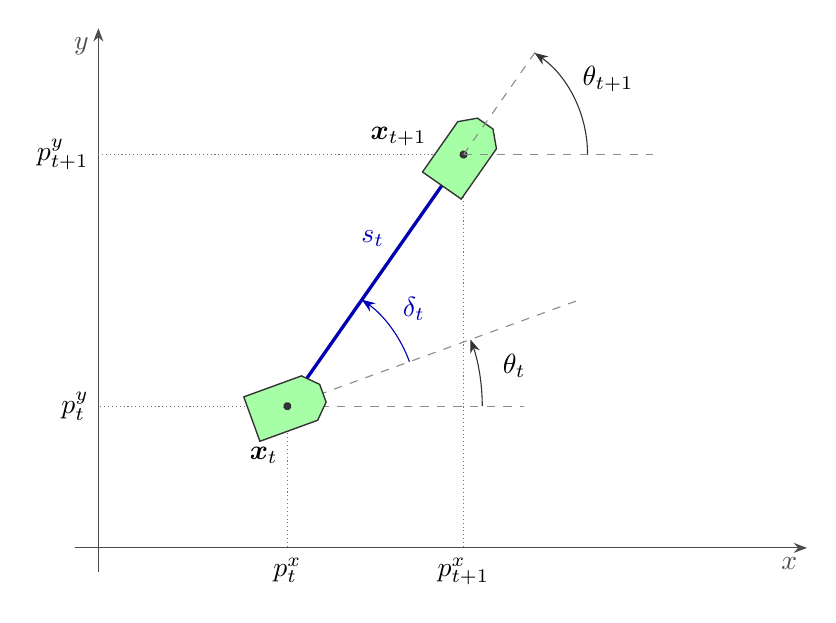
\begin{tikzpicture}[scale=1.5,>=Stealth,
    mower/.style={draw=black!80,fill=green!35,line width=0.5pt},
    proj/.style={densely dotted,black!55},
    ref/.style={dashed,black!45}]
  % axes
  \draw[->,black!70] (-0.2,0) -- (6.0,0) node[below left] {$x$};
  \draw[->,black!70] (0,-0.2) -- (0,4.4) node[below left] {$y$};
  % poses
  \coordinate (P) at (1.6,1.2);
  \def\th{20}\def\de{35}\def\s{2.6}
  \coordinate (Q) at ($(P)+({\s*cos(\th+\de)},{\s*sin(\th+\de)})$);
  % projections of x_t onto the axes
  \draw[proj] (P) -- (P |- 0,0) node[below,black] {$p^x_t$};
  \draw[proj] (P) -- (0,0 |- P) node[left,black] {$p^y_t$};
  \draw[proj] (Q) -- (Q |- 0,0) node[below,black] {$p^x_{t+1}$};
  \draw[proj] (Q) -- (0,0 |- Q) node[left,black] {$p^y_{t+1}$};
  % reference direction and old heading
  \draw[ref] (P) -- ++(2.0,0);
  \draw[ref] (P) -- ++(\th:2.6);
  \draw[->,black!80] (P) ++(0:1.65) arc[start angle=0,end angle=\th,radius=1.65];
  \node at ($(P)+({\th/2}:1.95)$) {$\theta_t$};
  \draw[->,blue!70!black] (P) ++(\th:1.1) arc[start angle=\th,
    end angle=\th+\de,radius=1.1];
  \node[blue!70!black] at ($(P)+({\th+\de/2}:1.35)$) {$\delta_t$};
  % the drive
  \draw[->,very thick,blue!70!black] (P) -- (Q)
    node[pos=0.6,above left=-1pt] {$s_t$};
  % mowers (top view: deck with a bevelled front, pointing along the heading)
  \foreach \c/\a in {P/\th,Q/{\th+\de}}{
    \begin{scope}[shift={(\c)},rotate=\a]
      \draw[mower] (-0.32,-0.2) -- (0.2,-0.2) -- (0.32,-0.08) -- (0.32,0.08)
        -- (0.2,0.2) -- (-0.32,0.2) -- cycle;
      \fill[black!80] (0,0) circle (0.035);
    \end{scope}}
  % heading of x_{t+1}
  \draw[ref] (Q) -- ++(1.6,0);
  \draw[ref] (Q) -- ++(\th+\de:1.1);
  \draw[->,black!80] (Q) ++(0:1.05) arc[start angle=0,end angle=\th+\de,
    radius=1.05];
  \node at ($(Q)+({(\th+\de)/2}:1.38)$) {$\theta_{t+1}$};
  \node at ($(P)+(-0.2,-0.42)$) {$\x_t$};
  \node at ($(Q)+(-0.55,0.15)$) {$\x_{t+1}$};
\end{tikzpicture}
\caption{The pose $\x_t=(p^x_t,p^y_t,\theta_t)$: the mower's position on the
lawn and its heading, measured anticlockwise from the $x$-axis. The
control $\uu_t=(s_t,\delta_t)$ first turns the mower by $\delta_t$, then
drives it a distance $s_t$ along the new heading, which gives
$\x_{t+1}=f(\x_t,\uu_t)$ with $\theta_{t+1}=\theta_t+\delta_t$.}
\label{fig:pose}
\end{figure}

The noise enters through the \emph{control}, not added to the state. This
is the physically right model: the wheels slip, so the mower drives a
little more or less than commanded ($\varepsilon_s$) and turns a little
more or less ($\varepsilon_\delta$). These are errors in the commands,
not yet in the position. The motion model converts them into position
errors through the $\cos$ and $\sin$ in \eqref{eq:f}: a distance error
moves the mower forward or backward \emph{along} its heading, whereas a
turn error changes the heading itself, and so moves the mower
\emph{sideways}, by an amount proportional to the distance driven. This
has two consequences that will follow us through the book.

\begin{proposition}{The transition is non-Gaussian and degenerate}{degenerate}
Fix $\x_t$ and $\uu_t$ with $s_t\neq0$.
\begin{enumerate}[label=(\roman*),nosep]
\item The distribution of $\x_{t+1}$ is not Gaussian.
\item It is concentrated on a two-dimensional surface of the
  three-dimensional state space, so it has no density with respect to
  the Lebesgue measure on $\R^3$.
\item Linearising $f$ in the noise gives the state-space covariance
  $Q_t=VMV\T$ with $V=\partial f/\partial\uu$, which has rank $2$.
\end{enumerate}
\end{proposition}

\begin{proof}
(ii) The map $\bepsilon\mapsto f(\x_t,\uu_t+\bepsilon)$ goes from $\R^2$
to $\R^3$ and is smooth, so its image is (at most) a two-dimensional
surface; $\x_{t+1}$ lies on it with probability one. A set of
three-dimensional Lebesgue measure zero carrying probability one rules out
a density. (i) A Gaussian on $\R^3$ is either non-degenerate (and has a
density) or supported on an affine subspace. The surface of (ii) is not
flat: the heading $\theta_{t+1}=\theta_t+\delta_t+\varepsilon_\delta$
enters the position through $\cos$ and $\sin$, so for a fixed step the
position runs along a circular arc as $\varepsilon_\delta$ varies.
(iii) With $\theta'=\theta+\delta$,
\[
  V=\begin{pmatrix}\cos\theta'&-s\sin\theta'\\ \sin\theta'&s\cos\theta'
  \\0&1\end{pmatrix}.
\]
Its two columns are independent when $s\neq0$ (the first has a zero third
entry, the second does not), so $V$ has rank 2 and so has $VMV\T$ since
$M$ is positive definite. Its null space is spanned by the cross product
of the columns, computed in Exercise~\ref{ex:nullspace}.
\end{proof}

\begin{inwords}
The pose space is three-dimensional: $(p^x,p^y,\theta)$. After one step
from a known pose, the new pose is fixed by only \emph{two} random
numbers, ``drove a bit more or less'' ($\varepsilon_s$) and ``turned a
bit more or less'' ($\varepsilon_\delta$). Three coordinates that depend on
two random inputs cannot fill a three-dimensional region: the reachable
poses form a two-dimensional sheet, and every pose off the sheet is
impossible. A Gaussian can only approximate it. After several steps the
noises of all the steps compound, the uncertainty fills all three
dimensions, but it stays curved: the familiar ``banana'' of
\cref{fig:transition}.
\end{inwords}

The sheet is easy to describe. Call $d=s+\varepsilon_s$ the distance
actually driven and $\varphi=\theta+\delta+\varepsilon_\delta$ the heading
actually reached. The reachable poses are
\[
  (d,\varphi)\longmapsto\bigl(p^x+d\cos\varphi,\;p^y+d\sin\varphi,\;
  \varphi\bigr),
\]
a \emph{helicoid}: the shape of a spiral staircase around the vertical
line through the start position (\cref{fig:helicoid}). At height $\varphi$
(a given heading), the possible positions form a straight segment pointing
in the direction $\varphi$; as the height increases, the segment rotates.
Each horizontal slice is straight, but the sheet twists, so it is not a
plane, and no Gaussian, whose level sets are ellipsoids, can follow it.
Its shadow on the lawn, the set of reachable positions, is an arc-shaped
band.

\begin{figure}[ht]
\centering
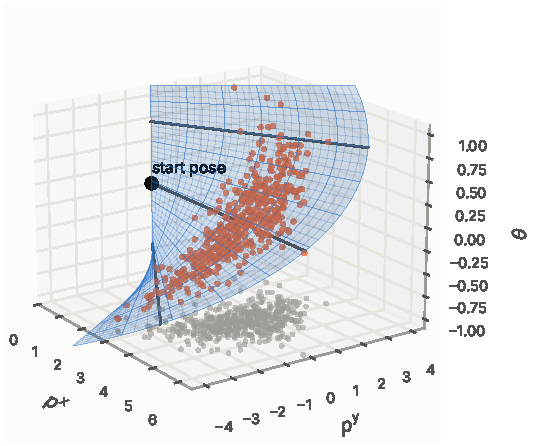
\includegraphics[width=0.72\linewidth]{figures/ch01_helicoid.pdf}
\caption{The poses reachable in one step from the start pose (black dot),
with the noise exaggerated for visibility ($\sigma_s=0.6$,
$\sigma_\delta=0.35$\,rad). Orange: 500 sampled poses $(p^x,p^y,\theta)$;
they all lie on a helicoid (blue), whose horizontal slices are the
straight segments of fixed heading (dark lines). Grey: their shadow on
the lawn, the positions alone, an arc-shaped band.}
\label{fig:helicoid}
\end{figure}

With the real noise of the simulations ($\sigma_s=0.4$,
$\sigma_\delta=0.03$), one step covers only a small patch of the
staircase, which looks almost flat. The curvature becomes visible as the
steps accumulate.

\begin{figure}[ht]
\centering
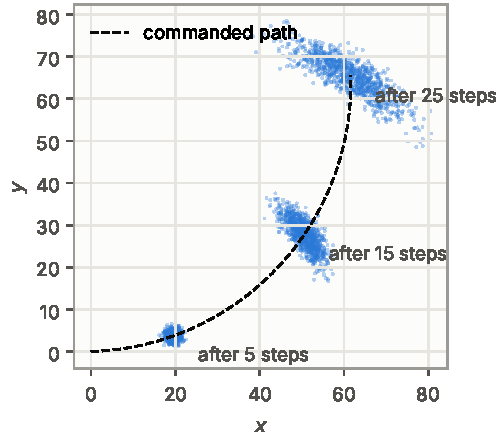
\includegraphics{figures/ch01_transition.pdf}
\caption{A thousand mowers start at the origin, heading east, and receive
the same 25 commands (drive 4, turn $\pi/50$). Their positions after 5,
15 and 25 steps. Only the positions are plotted: each cloud is the shadow
on the lawn of a cloud in the three-dimensional pose space, which after
several steps fills a curved volume rather than a single helicoid. Heading
errors become position errors \emph{across} the path, along arcs: the
clouds bend.}
\label{fig:transition}
\end{figure}

\section{Sensors}

Angles need one piece of notation. All headings and bearings are kept in
$[-\pi,\pi)$ by
\[
  \wrap(a)=a+2\pi k\quad\text{with the unique }k\in\mathbb{Z}\text{ such
  that }a+2\pi k\in[-\pi,\pi).
\]

\begin{lemma}{Angle differences}{wrap}
For angles $a,b$, $\wrap(a-b)$ is the signed rotation of smallest
magnitude that takes $b$ to $a$, and $\wrap(a-b)=\wrap(\wrap(a)-\wrap(b))$.
The plain difference $a-b$ of two wrapped angles can be off by $\pm2\pi$.
\end{lemma}

\begin{proof}
The rotations taking $b$ to $a$ are $a-b+2\pi k$, $k\in\mathbb{Z}$; exactly
one lies in $[-\pi,\pi)$, and it has the smallest magnitude (up to the tie
at $\pm\pi$). Since $\wrap(a)-a$ and $\wrap(b)-b$ are multiples of $2\pi$,
so is their difference, which $\wrap$ removes. For the last claim take
$a=3.10$ and $b=-3.12$: $a-b=6.22$, whereas $\wrap(a-b)=-0.063$.
\end{proof}

\begin{definition}{Range--bearing sensor}{rb}
The lawn holds $M$ landmarks (beacons) at known positions
$\bell_1,\dots,\bell_M$. For landmark $j$ let $\vect{d}=\bell_j-\p$, where
$\p=(p^x,p^y)$. The sensor returns
\begin{equation}\label{eq:h}
  \z_{t,j}=h_j(\x_t)+\vv_{t,j},\qquad
  h_j(\x)=\begin{pmatrix}\norm{\vect{d}}\\
  \wrap\bigl(\operatorname{atan2}(d_y,d_x)-\theta\bigr)\end{pmatrix},
  \qquad \vv_{t,j}\sim\Normal\bigl(\vect0,\,R_1\bigr),
\end{equation}
$R_1=\diag(\sigma_r^2,\sigma_\phi^2)$, for the landmarks within range,
with all $\vv_{t,j}$ independent. The bearing is measured \emph{relative to
the heading}, so it carries information about $\theta$.
\end{definition}

\begin{figure}[ht]
\centering
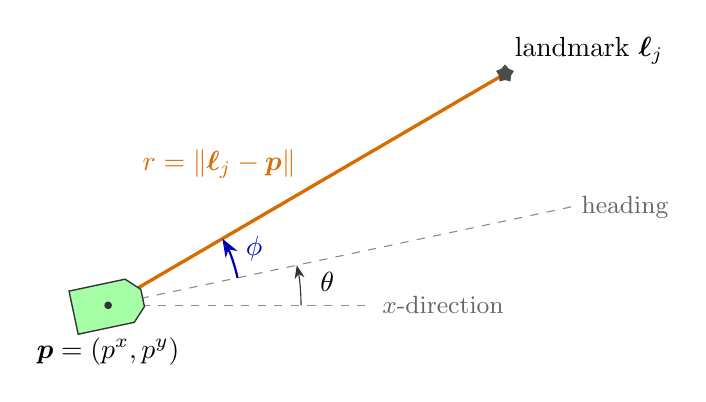
\begin{tikzpicture}[scale=1.4,>=Stealth,
    mower/.style={draw=black!80,fill=green!35,line width=0.5pt}]
  \coordinate (P) at (0,0);
  \coordinate (L) at (3.6,2.1);
  \def\th{12}
  \draw[dashed,black!45] (P) -- ++(2.4,0) node[right,black!60]
    {\small $x$-direction};
  \draw[dashed,black!45] (P) -- ++(\th:4.3) node[right,black!60]
    {\small heading};
  \draw[->,black!80] (P) ++(0:1.75) arc[start angle=0,end angle=\th,
    radius=1.75];
  \node at ($(P)+({\th/2}:2.0)$) {$\theta$};
  \draw[very thick,orange!85!black] (P) -- (L)
    node[midway,above left] {$r=\norm{\bell_j-\p}$};
  \draw[->,blue!70!black,thick] (P) ++(\th:1.2) arc[start angle=\th,
    end angle={atan2(2.1,3.6)},radius=1.2];
  \node[blue!70!black] at ($(P)+({(\th+atan2(2.1,3.6))/2}:1.42)$) {$\phi$};
  \begin{scope}[shift={(P)},rotate=\th]
    \draw[mower] (-0.32,-0.2) -- (0.2,-0.2) -- (0.32,-0.08) -- (0.32,0.08)
      -- (0.2,0.2) -- (-0.32,0.2) -- cycle;
    \fill[black!80] (0,0) circle (0.035);
  \end{scope}
  \node[below=8pt] at (P) {$\p=(p^x,p^y)$};
  \node[star,star points=5,fill=black!70,inner sep=1.6pt] at (L) {};
  \node[above right] at (L) {landmark $\bell_j$};
\end{tikzpicture}
\caption{The range--bearing measurement of landmark $j$. The range $r$ is
the distance from the mower to the landmark; the bearing $\phi$ is the
angle from the mower's heading to the line of sight, so that the direction
of the landmark in the lawn's frame is $\theta+\phi$.}
\label{fig:sensor}
\end{figure}

\Cref{fig:sensor} shows the two components of $h_j$.

Two simpler sensors are used in Chapters~\ref{ch:bayes}
and~\ref{ch:kalman}: a \emph{GPS-like position fix}
$\z_t=\p_t+\vv_t$, $\vv_t\sim\Normal(\vect0,\sigma_{\mathrm{gps}}^2I)$, and
a \emph{compass} $c_t=\wrap(\theta_t+\nu_t)$,
$\nu_t\sim\Normal(0,\sigma_c^2)$.

A last question is whether the sensor says \emph{which} landmark it saw.
When it does (\emph{known data association}) the measurement is the
indexed family $(\z_{t,j})_j$. When it does not, it is only the set of
$(r,\phi)$ pairs, and the filter must work out the correspondence itself
(\cref{sec:ekf-association,sec:pf-association}).

\section{The two assumptions}

\begin{definition}{Markov state and conditionally independent measurements}{markov}
\begin{enumerate}[label=(A\arabic*),nosep]
\item\label{A1} \emph{Markov motion}: given $\x_{t}$ and $\uu_t$, the
  next state is independent of all earlier states, controls and
  measurements:
  $p(\x_{t+1}\mid\x_{0:t},\uu_{0:t},\z_{1:t})=p(\x_{t+1}\mid\x_t,\uu_t)$.
\item\label{A2} \emph{Conditionally independent measurements}: given
  $\x_t$, the measurement $\z_t$ is independent of everything else:
  $p(\z_t\mid\x_{0:t},\uu_{0:t-1},\z_{1:t-1})=p(\z_t\mid\x_t)$.
\end{enumerate}
\end{definition}

Indices follow the code: control $\uu_t$ moves the mower from $\x_t$ to
$\x_{t+1}$, and $\z_{t+1}$ is measured at $\x_{t+1}$. Both assumptions
hold for the model above by construction, since the noises
$\bepsilon_t$ and $\vv_t$ are independent of everything else.

\begin{proposition}{Factorisation of the joint distribution}{joint}
Under \ref{A1}--\ref{A2}, for known controls $\uu_{0:T-1}$,
\begin{equation}\label{eq:joint}
  p(\x_{0:T},\z_{1:T}\mid\uu_{0:T-1})=p(\x_0)\prod_{t=0}^{T-1}
  p(\x_{t+1}\mid\x_t,\uu_t)\,p(\z_{t+1}\mid\x_{t+1}).
\end{equation}
\end{proposition}

\begin{proof}
Order the variables as $\x_0,\x_1,\z_1,\x_2,\z_2,\dots$ and apply the
chain rule of probability, conditioning each variable on all the previous
ones (and on the controls). The factor of $\x_{t+1}$ is
$p(\x_{t+1}\mid\x_{0:t},\z_{1:t},\uu_{0:T-1})$. Future controls carry no
information about the past motion (they are chosen in advance or from
past data), so this equals $p(\x_{t+1}\mid\x_{0:t},\z_{1:t},\uu_{0:t})$,
which is $p(\x_{t+1}\mid\x_t,\uu_t)$ by \ref{A1}. The factor of
$\z_{t+1}$ is $p(\z_{t+1}\mid\x_{0:t+1},\z_{1:t},\uu)$, which is
$p(\z_{t+1}\mid\x_{t+1})$ by \ref{A2}.
\end{proof}

\begin{inwords}
The whole story, every pose and every measurement, is a chain of small
local pieces: a start, then alternately ``move'' and ``look''. The state
is a sufficient summary of the past: once you know where the mower is,
how it got there is irrelevant to what happens next. That is exactly what
makes a \emph{recursive} filter possible, one that keeps only a belief
about the current state.
\end{inwords}

The densities in \eqref{eq:joint} are a convenient notation. By
\cref{prop:degenerate} the transition has no density on $\R^3$; the
identities in this book remain true with $p(\x_{t+1}\mid\x_t,\uu_t)$ read
as a transition \emph{kernel}, integrals as integrals against it. The
particle filter (\cref{ch:particle}) never needs the density at all: it
only \emph{samples} the motion.

\section{Why filter? Dead reckoning}

The simplest estimator ignores the sensors and integrates the commands:
$\hx_{t+1}=f(\hx_t,\uu_t)$ from the known start. This is \emph{dead
reckoning}. Its error is driven by the control noise, and grows without
bound.

\begin{proposition}{Dead-reckoning error on a straight path}{deadreckoning}
Let the mower start at a known pose heading along the $x$-axis and receive
$t$ commands $\uu=(s,0)$. Let $e_t=p^y_t$ be its lateral error and
$a_t=st-p^x_t$ its forward shortfall with respect to dead reckoning. Then
\begin{align}
  \theta_t&=\textstyle\sum_{k=1}^t\varepsilon_{\delta,k},
  & \Var(\theta_t)&=t\,\sigma_\delta^2,\label{eq:drheading}\\
  e_t&\approx s\textstyle\sum_{k=1}^t\theta_k,
  & \Var(e_t)&\approx s^2\sigma_\delta^2\,\frac{t(t+1)(2t+1)}{6},
  \label{eq:drlateral}\\
  \E[a_t]&\approx\frac{s\,\sigma_\delta^2}{4}\,t(t+1),
  \label{eq:drshort}
\end{align}
where $\approx$ means up to terms of higher order in the noise standard
deviations.
\end{proposition}

\begin{proof}
Heading errors simply add up, so $\theta_t$ is a sum of $t$ independent
$\Normal(0,\sigma_\delta^2)$ variables, which gives \eqref{eq:drheading}.
At step $k$ the mower moves by $(s+\varepsilon_{s,k})(\cos\theta_k,
\sin\theta_k)$. Its lateral component is $(s+\varepsilon_{s,k})
\sin\theta_k=s\theta_k+O(\varepsilon^2)$, so
$e_t\approx s\sum_k\theta_k=s\sum_{k=1}^t\sum_{j=1}^k\varepsilon_{\delta,j}
=s\sum_{j=1}^t(t-j+1)\varepsilon_{\delta,j}$. The variance of a sum of
independent terms is the sum of the variances:
$s^2\sigma_\delta^2\sum_{m=1}^t m^2$, which is \eqref{eq:drlateral}.
The forward displacement at step $k$ is
$(s+\varepsilon_{s,k})\cos\theta_k=s+\varepsilon_{s,k}-\tfrac s2\theta_k^2
+O(\varepsilon^3)$, so $\E[a_t]\approx\tfrac s2\sum_k\E[\theta_k^2]=
\tfrac s2\sigma_\delta^2\sum_k k$.
\end{proof}

\begin{inwords}
The lateral error grows like $t^{3/2}$, not like $\sqrt t$: each heading
error is \emph{integrated} along the rest of the path. Worse, the mower is
\emph{on average} short of where dead reckoning puts it, because a wrong
heading always shortens the forward progress. That bias, the
$\E[\cos\theta]<1$ effect, is invisible to any method that linearises the
motion, and will reappear in Chapter~\ref{ch:ekf}.
\end{inwords}

With the noise of the simulations ($s=4$, $\sigma_\delta=0.03$) and
$t=100$, \eqref{eq:drlateral} predicts a lateral standard deviation of
$69.8$ and \eqref{eq:drshort} a shortfall of $9.1$. A Monte Carlo run with
20\,000 mowers gives $67.5$ and $8.9$. On the figure-eight path of the
simulations the loops partly cancel the error (rotating a closed loop about
its start leaves its end in place), and the median error after 100 steps is
about 21; but it still grows without bound
(\cref{fig:deadreckoning}).

\begin{figure}[ht]
\centering
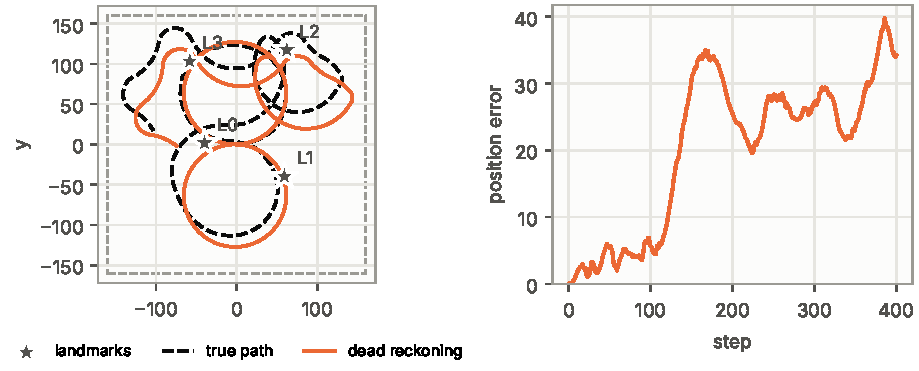
\includegraphics[width=\linewidth]{figures/ch01_dead_reckoning.pdf}
\caption{Dead reckoning on the standard run (seed 1). Left: the true path
and the integrated commands. Right: the position error. It is a random
walk, and nothing pulls it back.}
\label{fig:deadreckoning}
\end{figure}

A single GPS fix has the opposite problem: its error never grows, but it
never shrinks either (an RMS of $\sigma_{\mathrm{gps}}\sqrt2\approx11$ with
$\sigma_{\mathrm{gps}}=8$). A \emph{filter} combines the two: it uses the
motion model to carry information forward in time, and each new
measurement to correct the drift.

\begin{practice}[\nb{00\_the\_mower\_world.ipynb}, \code{world.py}]
\code{World} holds the lawn, the landmarks and the \emph{true} noise
levels; \code{motion\_model} and \code{range\_bearing} are $f$ and $h$,
vectorised over leading dimensions so that they also move whole clouds
of particles or sigma points. \code{simulate} returns a \code{Run} with the
true poses, the commanded controls and every sensor reading. The pilot of
the simulation steers the mower back towards the centre near the edges of
the lawn; that steering is part of the \emph{command}, so the filters know
it. The notebook draws \cref{fig:transition,fig:deadreckoning}.
\end{practice}

\begin{mower}
On a real mower the control is the odometry reported by the wheel
encoders, not the command sent to the motors, and its noise depends on
the ground: much larger on wet grass or a slope, where the wheels slip.
Those are also the conditions in which the heading error, and therefore
the $t^{3/2}$ growth, is worst. A robot mower that relied on odometry
alone would drift off its stripes within a few metres. This is why every
commercial one has a second source of position: a boundary wire, beacons,
RTK-GNSS or a camera.
\end{mower}

\FloatBarrier
\section*{Exercises}
\addcontentsline{toc}{section}{Exercises}

\begin{enumerate}[label=\textbf{1.\arabic*},ref=1.\arabic*]
\item\label{ex:nullspace} Compute the null space of $Q=VMV\T$ from
  \cref{prop:degenerate}. Which combination of position and heading
  errors can a single step never produce, to first order?
\item\label{ex:ecos} Let $\theta\sim\Normal(0,\sigma^2)$. Show that
  $\E[\cos\theta]=e^{-\sigma^2/2}$ and $\E[\sin\theta]=0$. Deduce the
  exact mean forward progress of one noisy step from a heading known up to
  $\Normal(0,\sigma^2)$, and compare it with the linearised value $s$.
\item\label{ex:condind} Using \cref{prop:joint}, show that the
  measurements are \emph{not} independent of one another, but that they
  are independent given the states: $p(\z_{1:T}\mid\x_{0:T})=
  \prod_t p(\z_t\mid\x_t)$.
\item\label{ex:wrapadd} Is $\wrap$ additive, i.e.\ is
  $\wrap(a+b)=\wrap(a)+\wrap(b)$? Give a proof or a counter-example, and
  explain why the code wraps the heading \emph{after} each update.
\end{enumerate}

\subsection*{Solutions}

\textbf{1.1.} The null space of $VMV\T$ equals the null space of $V\T$
because $M$ is positive definite. A vector $\vect{n}$ with $V\T\vect{n}=
\vect0$ is orthogonal to both columns of $V$, so it is their cross
product:
\[
  \vect{n}=\begin{pmatrix}\cos\theta'\\\sin\theta'\\0\end{pmatrix}\times
  \begin{pmatrix}-s\sin\theta'\\s\cos\theta'\\1\end{pmatrix}
  =\begin{pmatrix}\sin\theta'\\-\cos\theta'\\s\end{pmatrix}.
\]
To first order, the error $\Delta\x$ of one step satisfies
$\vect{n}\T\Delta\x=0$, i.e.\ $\Delta_{\perp}=s\,\Delta\theta$, where
$\Delta_\perp=-\sin\theta'\Delta p^x+\cos\theta'\Delta p^y$ is the
sideways position error: a sideways error can only come from having turned
wrongly, and the two are tied. A sideways jump with the right heading is
impossible.

\textbf{1.2.} $\E[e^{i\theta}]=e^{-\sigma^2/2}$ is the characteristic
function of $\Normal(0,\sigma^2)$ at $1$. Its real and imaginary parts
are $\E[\cos\theta]$ and $\E[\sin\theta]$; the second is also $0$ because
$\sin$ is odd and the distribution symmetric. A step of length $s$ in
direction $\theta$ therefore advances by $s\,e^{-\sigma^2/2}<s$ on
average. Linearising $\cos\theta\approx1$ gives $s$, and the bias
$s(1-e^{-\sigma^2/2})\approx s\sigma^2/2$ is exactly the per-step term in
\eqref{eq:drshort}.

\textbf{1.3.} Integrating \eqref{eq:joint} over $\x_{0:T}$ gives
$p(\z_{1:T}\mid\uu)$, which does not factorise: two measurements both
depend on the trajectory, which is random (two GPS fixes taken one step
apart are strongly correlated because the mower was nearly in the same
place). Dividing \eqref{eq:joint} by $p(\x_{0:T}\mid\uu)=p(\x_0)\prod_t
p(\x_{t+1}\mid\x_t,\uu_t)$, which is the marginal of \eqref{eq:joint}
obtained by integrating out every $\z_t$ (each likelihood integrates to
one), leaves $\prod_t p(\z_t\mid\x_t)$.

\textbf{1.4.} No: $\wrap(3+3)=6-2\pi\approx-0.28$, whereas
$\wrap(3)+\wrap(3)=6$. $\wrap$ is additive only modulo $2\pi$:
$\wrap(a+b)=\wrap(\wrap(a)+\wrap(b))$. A filter update adds a correction
$K\y$ to the heading; the sum may leave $[-\pi,\pi)$, and if it is not
wrapped, the next innovation (a difference of angles,
\cref{lem:wrap}) or the next circular mean will treat a heading of
$3.2$ and one of $-3.08$ as different, although they are the same
direction.

\chapter{The Bayes filter}
\label{ch:bayes}

Every filter in this book is an approximation of one recursion. This
chapter derives it, from the two assumptions of
Chapter~\ref{ch:statespace} and nothing else, and then implements it with
no approximation other than discretisation: on a grid. The grid shows what
the exact belief looks like (sometimes it has two separate bumps) and why
we cannot afford a grid in general.

\section{Belief}

The robot never knows its pose exactly. What it knows is described by a
probability distribution over the possible poses: sharp when it is sure,
spread out when it is not, with several bumps when several places fit what
it has seen. This distribution is what a filter computes.

Three words come back all the time. A distribution of the state held
\emph{before} a measurement is taken into account is called a
\emph{prior}; the distribution \emph{after} it is the \emph{posterior}.
And $p(\z\mid\x)$, read as a function of the state $\x$ for the
measurement $\z$ actually received, is the \emph{likelihood}: it says how
well each possible state explains that measurement.

\paragraph{What the value of a likelihood means.} The number
$p(\z\mid\x)$ is not the probability of receiving $\z$: for a continuous
measurement the probability of any exact value is zero. It is the value of
a density, a probability per unit volume (\cref{sec:shape}). For a small
region $B$ around the reading that was received,
\[
  \Pr(\z\in B\mid\x)\approx p(\z\mid\x)\times\text{volume of }B .
\]
The volume of $B$ is the same whatever the state $\x$. So comparing two
states by their likelihoods is comparing the probabilities that they give
to ``a reading close to the one received'': if
$p(\z\mid\x)=3\,p(\z\mid\x')$, such a reading is three times more
probable from $\x$ than from $\x'$. This is also what a sensor really
delivers, since its resolution is finite: a small cell, not an exact
value.

This is what makes it legitimate to weigh the states by their likelihood,
as Bayes' rule does below, and to prefer the state under which the
measurement is the most likely, the \emph{maximum-likelihood} choice
(used in \cref{sec:ekf-association} to decide which landmark a reading
comes from). Two cautions go with it.
\begin{itemize}[nosep]
  \item The likelihood is a density in $\z$, not in $\x$: read as a
    function of $\x$ it need not integrate to one, and only ratios between
    states have a meaning. Changing the unit of $\z$ multiplies all the
    likelihoods by the same factor and changes no ratio.
  \item It ranks the states by how well they explain the measurement. It
    does not say how probable a state is: that needs a prior as well, and
    is the posterior.
\end{itemize}

\begin{definition}{Belief and predicted belief}{belief}
The \emph{belief} at step $t$ is the posterior distribution of the
current state given everything observed so far,
\[
  \bel(\x_t)=p(\x_t\mid\z_{1:t},\uu_{0:t-1}),
\]
and the \emph{predicted belief} is the distribution of the next state
after the next control but before the next measurement,
\[
  \belbar(\x_{t+1})=p(\x_{t+1}\mid\z_{1:t},\uu_{0:t}).
\]
\end{definition}

The belief is the complete answer to ``where is the robot?''. A filter
may summarise it (by its mean and covariance, say), but every summary
loses information, and some summaries can be badly misleading
(\cref{sec:twobumps}). Before any measurement, the belief is the
distribution of the start pose, $\bel(\x_0)=p(\x_0)$: concentrated around
one pose if the start is known, wide if it is not. (A start that is known
exactly would be a single point, a distribution without a density; in
practice the start is always given a small spread.)

\section{The recursion}

The belief can be computed step by step: the belief at step $t+1$ is
obtained from the belief at step $t$, the control $\uu_t$ and the
measurement $\z_{t+1}$, with no need to go back to older data
(\cref{fig:bayesflow}). Each cycle has two stages: \emph{predict}, which
accounts for the motion, and \emph{update}, which accounts for the
measurement.

\begin{figure}[ht]
\centering
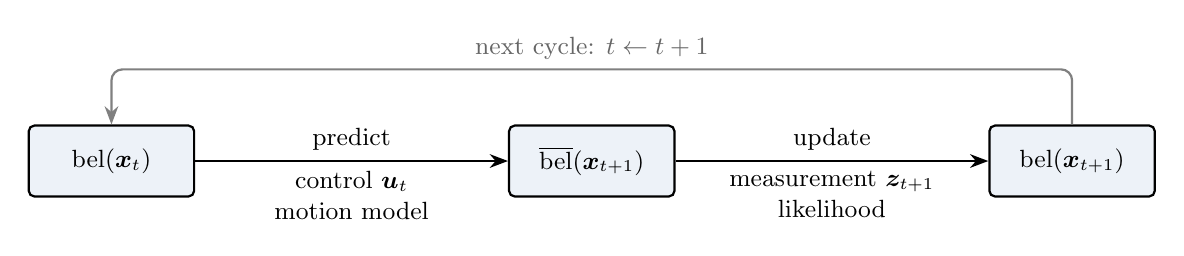
\begin{tikzpicture}[>=Stealth,
  box/.style={draw,thick,rounded corners=2pt,minimum height=9mm,
    minimum width=21mm,font=\small,fill=defblue!8},
  lab/.style={font=\small,align=center}]
  \node[box] (b0) at (0,0) {$\bel(\x_t)$};
  \node[box] (bb) at (6.1,0) {$\belbar(\x_{t+1})$};
  \node[box] (b1) at (12.2,0) {$\bel(\x_{t+1})$};
  \draw[->,thick] (b0) -- (bb) node[pos=0.5,above,lab] {predict}
    node[pos=0.5,below,lab] {control $\uu_t$\\motion model};
  \draw[->,thick] (bb) -- (b1) node[pos=0.5,above,lab] {update}
    node[pos=0.5,below,lab] {measurement $\z_{t+1}$\\likelihood};
  \draw[->,thick,black!50,rounded corners=4pt] (b1.north) -- ++(0,0.7)
    -| (b0.north) node[pos=0.25,above,font=\small,black!60]
    {next cycle: $t\leftarrow t+1$};
\end{tikzpicture}
\caption{One cycle of the Bayes filter. The predict step turns the belief
into the predicted belief, using the control and the motion model. The
update step turns the predicted belief into the new belief, using the
measurement and its likelihood.}
\label{fig:bayesflow}
\end{figure}

When the state takes only a few values, a cycle can be done by hand.

\begin{example}{A two-state filter}{grassgravel}
The robot is either on the grass ($G$) or on the gravel path ($P$). At
each step it stays on the same surface with probability $0.9$. A vibration
sensor says ``rough'' with probability $0.8$ on gravel and $0.3$ on grass.
The current belief is $\bel=(0.8,\,0.2)$ for $(G,P)$: the robot is
probably on the grass.

\emph{Predict.} The robot is on the grass at the next step if it was on
the grass and stayed, or on the path and left it:
$\belbar(G)=0.9\times0.8+0.1\times0.2=0.74$, and
$\belbar(P)=0.1\times0.8+0.9\times0.2=0.26$. The belief has moved towards
$(0.5,0.5)$: it is less sure than before.

\emph{Update.} The sensor says ``rough''. Multiply the predicted
probability of each state by the probability that this state gives the
reading ``rough'', $p(\text{rough}\mid G)=0.3$ and
$p(\text{rough}\mid P)=0.8$: $0.3\times0.74=0.222$ for $G$ and
$0.8\times0.26=0.208$ for $P$.

These two products are not yet the new belief. Each is the probability of
two things together: $0.222$ is the probability that the robot is on the
grass \emph{and} the sensor says ``rough'' (probability $0.74$ to be on
the grass, then $0.3$ that the grass gives ``rough''), and $0.208$ the
probability that it is on the path \emph{and} the sensor says ``rough''.
These are the only two ways of getting the reading ``rough'', so their sum
\[
  0.222+0.208=0.43
\]
is the probability of the reading ``rough'' itself, computed from the
predicted belief: the probability that the filter gave to this reading
before seeing it. Before the reading arrives, there are four possible
cases, a surface and a reading, and their probabilities add up to $1$:
\begin{center}
\begin{tabular}{lccc}
  \toprule
  & ``rough'' & ``smooth'' & total\\
  \midrule
  grass ($0.74$) & $0.74\times0.3=0.222$ & $0.74\times0.7=0.518$ & $0.74$\\
  path ($0.26$)  & $0.26\times0.8=0.208$ & $0.26\times0.2=0.052$ & $0.26$\\
  \midrule
  total & $0.43$ & $0.57$ & $1$\\
  \bottomrule
\end{tabular}
\end{center}
The sensor says ``rough'': the column ``smooth'' becomes impossible and is
struck out. Only the two cases of the column ``rough'' remain, and the new
belief is the share of each in their total:
\[
  \bel(G)=\frac{0.222}{0.43}=0.516,\qquad
  \bel(P)=\frac{0.208}{0.43}=0.484 .
\]
Dividing by $0.43$ is what makes the two new probabilities add up to $1$;
it does not change their ratio, which the products already fixed. One
rough reading has almost cancelled the initial confidence in the grass.
(The sum is the rule of total probability, and the division is Bayes'
rule, both recalled below.)
\end{example}

The general recursion is the same computation, with integrals over the
state in place of the sums over two values. Its derivation uses two rules
of probability, recalled here for densities.
\begin{itemize}[nosep]
  \item \emph{Total probability}: $p(a)=\int p(a\mid b)\,p(b)\,\mathrm db$.
    To find how likely $a$ is, go through every possible $b$.
  \item \emph{Bayes' rule}: $p(b\mid a)=p(a\mid b)\,p(b)/p(a)$. It turns
    ``how likely is this observation if the state is $b$'' into ``how
    likely is the state $b$ given this observation''.
\end{itemize}
Both remain true when every term is conditioned on the same extra
variables, which is how they are used below.

\begin{theorem}{Bayes filter}{bayes}
Under \ref{A1}--\ref{A2}, with controls fixed in advance or computed from
the measurements (the two cases of \cref{prop:joint}),
\begin{align}
  \belbar(\x_{t+1})&=\int p(\x_{t+1}\mid\x_t,\uu_t)\,\bel(\x_t)\,
  \mathrm d\x_t, \label{eq:predict}\\
  \bel(\x_{t+1})&=\eta_{t+1}\,p(\z_{t+1}\mid\x_{t+1})\,
  \belbar(\x_{t+1}),\qquad
  \eta_{t+1}^{-1}=\int p(\z_{t+1}\mid\x)\,\belbar(\x)\,\mathrm d\x.
  \label{eq:update}
\end{align}
\end{theorem}

\begin{proof}
Recall what the two beliefs are (\cref{def:belief}):
$\bel(\x_t)=p(\x_t\mid\z_{1:t},\uu_{0:t-1})$, the pose given all the data
up to step $t$, and $\belbar(\x_{t+1})=p(\x_{t+1}\mid\z_{1:t},\uu_{0:t})$,
the next pose given the same data and the control $\uu_t$. The proof
follows \cref{ex:grassgravel} step by step, with integrals in place of
sums.

\emph{Predict, step 1: go through every current pose.} The robot reaches
$\x_{t+1}$ from some current pose $\x_t$. The law of total probability,
with everything conditioned on the data $(\z_{1:t},\uu_{0:t})$, adds up
the ways of reaching $\x_{t+1}$, one for each $\x_t$:
\[
  \underbrace{p(\x_{t+1}\mid\z_{1:t},\uu_{0:t})}_{\belbar(\x_{t+1})}
  =\int p(\x_{t+1}\mid\x_t,\z_{1:t},\uu_{0:t})\;
  p(\x_t\mid\z_{1:t},\uu_{0:t})\,\mathrm d\x_t .
\]
In the example this was $\belbar(G)=0.9\times0.8+0.1\times0.2$: the
probability of moving to $G$ from each state, times the probability of
that state.

\emph{Predict, step 2: the first factor is the motion model.} \ref{A1}
removes everything but $\x_t$ and $\uu_t$: it says that, given $\x_t$ and
$\uu_t$, the next pose is independent of all the earlier variables
together, hence also of those that appear here, $\z_{1:t}$ and
$\uu_{0:t-1}$. This includes the last measurement $\z_t$: the next pose
is $f(\x_t,\uu_t+\bepsilon_t)$, in which no measurement appears. A
measurement can act on the motion only through the control, when the
control is computed from it, and the control $\uu_t$ is given. So the
first factor is $p(\x_{t+1}\mid\x_t,\uu_t)$.

\emph{Predict, step 3: the second factor is the belief.} The control
$\uu_t$ carries no information about $\x_t$ beyond what is already given
(it is fixed in advance, or computed from the measurements $\z_{1:t}$),
so it can be dropped, which leaves
$p(\x_t\mid\z_{1:t},\uu_{0:t-1})=\bel(\x_t)$ (\cref{sec:bayesnet-mower},
statement~(c), checks this independence on the graph of the model).
Substituting both factors gives \eqref{eq:predict}.

\emph{Update, step 1: Bayes' rule.} Now the measurement $\z_{t+1}$
arrives. Bayes' rule, with everything conditioned on the data
$(\z_{1:t},\uu_{0:t})$ already in hand, gives
\[
  \underbrace{p(\x_{t+1}\mid\z_{1:t+1},\uu_{0:t})}_{\bel(\x_{t+1})}=
  \frac{p(\z_{t+1}\mid\x_{t+1},\z_{1:t},\uu_{0:t})\;
  p(\x_{t+1}\mid\z_{1:t},\uu_{0:t})}
  {p(\z_{t+1}\mid\z_{1:t},\uu_{0:t})}.
\]
(Bayes' rule itself comes from writing the probability of $\x_{t+1}$ and
$\z_{t+1}$ together in two ways: $p(\x_{t+1}\mid\z_{t+1})\,p(\z_{t+1})=
p(\z_{t+1}\mid\x_{t+1})\,p(\x_{t+1})$, all conditioned on the data, and
dividing by $p(\z_{t+1})$.)

\emph{Update, step 2: the numerator.} \ref{A2} reduces its first factor
to $p(\z_{t+1}\mid\x_{t+1})$ (given $\x_{t+1}$, the measurement is
independent of all the earlier variables, hence of $\z_{1:t}$ and
$\uu_{0:t}$), and its second factor is $\belbar(\x_{t+1})$. The numerator
is therefore $p(\z_{t+1}\mid\x_{t+1})\,\belbar(\x_{t+1})$: the probability
of being at $\x_{t+1}$ \emph{and} receiving the reading $\z_{t+1}$, the
products $0.222$ and $0.208$ of the example.

\emph{Update, step 3: the denominator.} It is the probability of the
reading $\z_{t+1}$ given the data, before knowing where the robot is: the
$0.43$ of the example. It is computed like $0.43=0.222+0.208$, by going
through every possible next pose (total probability again, then \ref{A2}
in the first factor):
\[
  p(\z_{t+1}\mid\z_{1:t},\uu_{0:t})
  =\int p(\z_{t+1}\mid\x,\z_{1:t},\uu_{0:t})\,
   p(\x\mid\z_{1:t},\uu_{0:t})\,\mathrm d\x
  =\int p(\z_{t+1}\mid\x)\,\belbar(\x)\,\mathrm d\x ,
\]
the integral of the numerator over all the poses. This is
$\eta_{t+1}^{-1}$, and the three steps together give \eqref{eq:update}.

\emph{A check.} The denominator does not depend on $\x_{t+1}$, and
dividing by it is exactly what makes the new belief integrate to one:
integrating \eqref{eq:update} over $\x_{t+1}$ gives
$\eta_{t+1}\int p(\z_{t+1}\mid\x)\,\belbar(\x)\,\mathrm d\x=1$. As in the
example, the division fixes the total, not the shape: the shape of the
new belief is set by the numerator alone. This is why the denominator is
often called a \emph{normalising constant}.
\end{proof}

\paragraph{What is a density in these formulas, and what is not.} The
beliefs $\bel$ and $\belbar$ and the likelihood $p(\z\mid\x)$ are
densities: functions that can be evaluated and integrated (the initial
belief $p(\x_0)$ is assumed to have one). The transition
$p(\x_{t+1}\mid\x_t,\uu_t)$ is a distribution \emph{without} a density
(\cref{prop:degenerate}), so \eqref{eq:predict} cannot be read as the
integral of a product of two functions. Here is how it is read instead, in
three steps.

\emph{What \eqref{eq:predict} means.} Go through every current pose
$\x_t$, weighted by its belief $\bel(\x_t)$, and spread it over the poses
it can move to with the control $\uu_t$; $\belbar$ collects all these
spreads. The trouble is only in the spread of one pose: it lies on a thin
surface (\cref{fig:transition}), so it has no density to multiply by
$\bel(\x_t)$.

\emph{The same thing as a recipe.} The spread of one pose $\x$ is the set
of poses $f(\x,\uu_t+\bepsilon)$ for all the possible control noises
$\bepsilon$, weighted by the density of the noise. So a predicted pose is
produced in three moves: draw a current pose $\x$ from $\bel$, draw a
noise $\bepsilon$ from $\Normal(\vect0,M)$, independently, and compute
$f(\x,\uu_t+\bepsilon)$. $\belbar$ is the distribution of the poses
produced this way. The recipe uses only $\bel$, the noise density and the
function $f$, which all exist.

\emph{The same thing as a formula.} A distribution is known once the
average under it of every function $g$ of the pose is known (as in
\cref{sec:assumptions}: $g(\x)=\x$ gives the mean, and the indicator of a
region, $1$ inside and $0$ outside, gives the probability of the region).\footnote{This
view of a distribution, through the averages it gives to functions, is
developed in the companion book (Section~20.7 there), with the
distributions of L.~Schwartz and the $\delta$ notation in which
\eqref{eq:predict} is often written.}
The average of $g$ over the predicted pose can be computed in two ways.
With the density $\belbar$, it is $\int g(\x)\,\belbar(\x)\,\mathrm d\x$.
With the recipe, the predicted pose is $f(\x,\uu_t+\bepsilon)$, where the
pair $(\x,\bepsilon)$ has the density $\bel(\x)\,\rho(\bepsilon)$ (a
product, since the two are drawn independently; $\rho$ is the Gaussian
density of the noise). The two must agree:
\begin{equation}\label{eq:predictnoise}
  \int g(\x)\,\belbar(\x)\,\mathrm d\x
  =\iint g\bigl(f(\x,\uu_t+\bepsilon)\bigr)\,\bel(\x)\,\rho(\bepsilon)\,
  \mathrm d\x\,\mathrm d\bepsilon .
\end{equation}
Every function in this equation can be evaluated: it is \eqref{eq:predict}
with nothing left to interpret. With $g(\x)=\x$, for instance, it says
that the mean of the predicted pose is the average of
$f(\x,\uu_t+\bepsilon)$ over the current poses and the noises.

This is also how the filters of the next chapters compute the prediction:
they push poses and noises through $f$, as in the recipe, and never
evaluate the transition. \Cref{sec:shape} explains why $\belbar$ has a
density when $\bel$ has one. The update \eqref{eq:update} involves
densities only.

\begin{inwords}
\emph{Predict}: push the belief through the motion model. Every possible
current pose spreads into the poses it could move to, weighted by how
likely it was. The belief blurs. \emph{Update}: reweight every pose by how
well it explains what was just seen, then renormalise. The belief
sharpens. Repeat.
\end{inwords}

\Cref{fig:bayescycle} shows one cycle on a one-dimensional example, where
everything can be computed exactly.

\begin{figure}[ht]
\centering
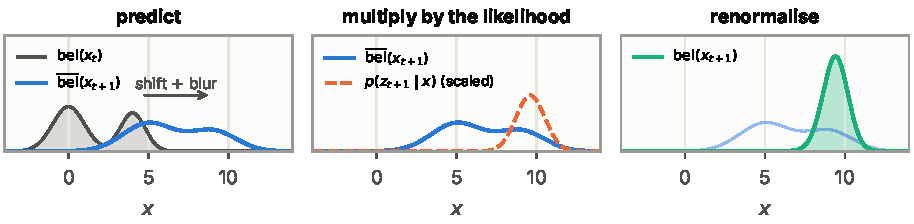
\includegraphics[width=\linewidth]{figures/ch02_bayes_cycle.pdf}
\caption{One cycle of the Bayes filter, computed exactly on a fine 1-D
grid. Predict: a two-bump belief is shifted by the commanded displacement
and blurred by the motion noise. Update: the prediction is multiplied by
the likelihood of the new measurement (dashed) and renormalised. The bump
that agrees with the measurement survives; the other one almost
disappears.}
\label{fig:bayescycle}
\end{figure}


The normaliser has a meaning of its own, which the particle filter will
use in \cref{sec:amcl}.

\begin{proposition}{The normaliser is the predictive likelihood}{evidence}
$\eta_{t+1}^{-1}=p(\z_{t+1}\mid\z_{1:t},\uu_{0:t})$, the value of the
density that the filter assigned to the measurement before seeing it.
For controls fixed in advance, the whole sequence of measurements has the
density
\[
  \log p(\z_{1:T}\mid\uu_{0:T-1})=-\sum_{t=1}^T\log\eta_t ,
\]
and when the controls are computed from the measurements the same sum is
$\log p(\z_{1:T})$.
\end{proposition}

\begin{proof}
\emph{The first claim.} It was obtained in the proof of \cref{thm:bayes}
(update, step~3): the denominator of Bayes' rule is
$p(\z_{t+1}\mid\z_{1:t},\uu_{0:t})$, and it equals
$\int p(\z_{t+1}\mid\x)\,\belbar(\x)\,\mathrm d\x=\eta_{t+1}^{-1}$. With
the index shifted by one, for every $t\ge1$,
\begin{equation}\label{eq:etat}
  \eta_t^{-1}=p(\z_t\mid\z_{1:t-1},\uu_{0:t-1}),
\end{equation}
the density of the measurement $\z_t$ given everything the filter had
before it: the earlier measurements and the controls already applied
(for $t=1$, $\z_{1:0}$ is empty).

\emph{Controls fixed in advance, step 1: the chain rule.} The density of
all the measurements together, given all the controls, is a product of
one factor per measurement, each conditioned on the measurements before
it (the chain rule, $p(a,b)=p(a)\,p(b\mid a)$ applied repeatedly):
\begin{align*}
  p(\z_{1:T}\mid\uu_{0:T-1})
  &=p(\z_1\mid\uu_{0:T-1})\,p(\z_2\mid\z_1,\uu_{0:T-1})\cdots
   p(\z_T\mid\z_{1:T-1},\uu_{0:T-1})\\
  &=\prod_{t=1}^Tp(\z_t\mid\z_{1:t-1},\uu_{0:T-1}).
\end{align*}

\emph{Step 2: compare each factor with \eqref{eq:etat}.} The factor of
$\z_t$ is conditioned on all the controls, $\uu_{0:T-1}$; \eqref{eq:etat}
only on those applied before $\z_t$, $\uu_{0:t-1}$. The difference is the
later controls $\uu_t,\dots,\uu_{T-1}$, and the factors are equal if
these carry no information about $\z_t$ given the rest, that is if
\[
  \z_t\indep\uu_{t:T-1}\mid\z_{1:t-1},\uu_{0:t-1}.
\]
That they are applied after $\z_t$ is not a reason: a conditional density
is about information, not influence (the trap of \cref{sec:assumptions}),
and a later control computed from $\z_t$ would carry information about
it. The reason is the graph of the model (\cref{fig:bayesnet}), read with
the d-separation rule (\cref{def:dsep}). Take a later control $\uu_s$,
$s\ge t$. Fixed in advance, it has no parent, and its only arrow is
$\uu_s\rightarrow\x_{s+1}$. So a path from $\uu_s$ to $\z_t$ starts
$\uu_s\rightarrow\x_{s+1}$, and from $\x_{s+1}$ it must go on along
another arrow: to $\z_{s+1}$ or $\x_{s+2}$, which lead only further into
the future and never back to $\z_t$, or to $\x_s$, along
$\x_{s+1}\leftarrow\x_s$. On every path that reaches $\z_t$, the node
$\x_{s+1}$ therefore has two arrows pointing into it,
$\uu_s\rightarrow\x_{s+1}\leftarrow\x_s$: it is a collider. A collider
blocks the path unless it, or one of its descendants, is given. The
descendants of $\x_{s+1}$ are the later poses and their measurements
$\z_{s+1},\z_{s+2},\dots$, all after $\z_t$; the given variables,
$\z_{1:t-1}$ and $\uu_{0:t-1}$, contain none of them, nor $\x_{s+1}$.
So every path is blocked, and \cref{thm:dsep} gives the independence.

\emph{Step 3: conclude.} Each factor is therefore
$p(\z_t\mid\z_{1:t-1},\uu_{0:t-1})=\eta_t^{-1}$, so
$p(\z_{1:T}\mid\uu_{0:T-1})=\prod_{t=1}^T\eta_t^{-1}$, and taking the
logarithm turns the product into the sum
$-\sum_{t=1}^T\log\eta_t$.

\emph{Controls computed from the measurements.} Now the controls are not
given in advance: $\uu_t=\pi_t(\z_{1:t})$, and the model is the joint
distribution $p(\x_{0:T},\z_{1:T})$ of \cref{prop:joint}(ii). Apply the
chain rule to $p(\z_{1:T})$ itself:
$p(\z_{1:T})=\prod_{t=1}^Tp(\z_t\mid\z_{1:t-1})$. In the factor of $\z_t$
the controls $\uu_0,\dots,\uu_{t-1}$ do not appear, but they are known:
each $\uu_s=\pi_s(\z_{1:s})$, $s\le t-1$, is computed from the
measurements $\z_{1:t-1}$ that are given. Adding to the condition a
variable that is a function of what is already given adds no
information, so
$p(\z_t\mid\z_{1:t-1})=p(\z_t\mid\z_{1:t-1},\uu_{0:t-1})=\eta_t^{-1}$,
and the same sum is $\log p(\z_{1:T})$.
\end{proof}

\begin{inwords}
The proposition gives the filter a measure of its own surprise, which it
computes anyway, since $\eta_t$ is the normaliser of every update.
$\eta_t^{-1}$ is the density that the filter, \emph{before} $\z_t$
arrived, gave to the value that then arrived: the $0.43$ of
\cref{ex:grassgravel}. A value as large as usual means the reading was
about as expected; a much smaller one means the filter had considered it
unlikely. One small value can be bad luck. A run of them cannot be
explained that way: by the second part of the proposition, the product of
the $\eta_t^{-1}$ over a stretch of time is the density that the model
gives to that whole stretch of readings, and a run of small factors makes
it tiny. The model then no longer explains the data: for example the
robot has been picked up and moved. \Cref{sec:amcl} uses exactly this
test to detect such a kidnapping, comparing a short-term average of
$\eta_t^{-1}$ with a long-term one.
\end{inwords}

\section{The grid filter}
\label{sec:grid}

Neither integral of \cref{thm:bayes} has a closed form in general. The
most direct approximation replaces the state space by a finite grid. To
keep the grid two-dimensional, the robot is given a compass
(\cref{sec:sensors}). The compass is accurate ($\sigma_c=0.02$\,rad, about
$1^\circ$), so the heading is taken from its reading and treated as known,
and only the position is uncertain. The state is then the position
$\p_t$ alone.

\begin{definition}{Grid belief}{grid}
Partition the lawn into $n$ square cells $C_1,\dots,C_n$, with centres
$\vect{c}_1,\dots,\vect{c}_n$. The \emph{grid belief} is the vector
$b_i\approx\Pr(\p_t\in C_i\mid\z_{1:t},\uu_{0:t-1})$, with $\sum_ib_i=1$.
\end{definition}

The \emph{convolution} of two functions on the plane is
\[
  (a\ast g)(\p)=\int a(\p-\vect q)\,g(\vect q)\,\mathrm d\vect q .
\]
\begin{figure}[t]
\centering
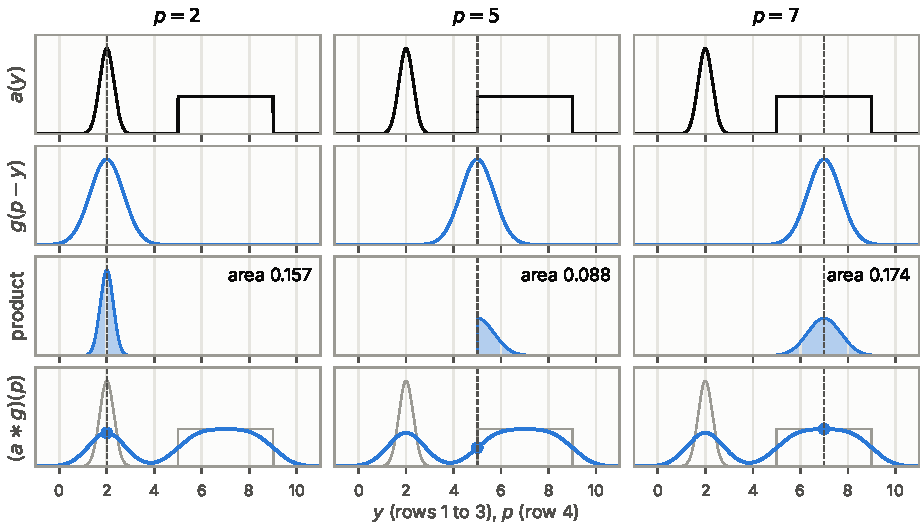
\includegraphics[width=\linewidth]{figures/ch02_conv_read.pdf}
\caption{Computing $a\ast g$ on the line, with $g=\Normal(0,0.7^2)$ and a
function $a$ made of a peak and a plateau (row~1). Each column is one
point $p$ (dashed line). Row~2: the weight $g(p-y)$ given to each value
$a(y)$, centred at $p$. Row~3: the product of the two, whose area is
$(a\ast g)(p)$. Row~4: $a\ast g$ at every $p$ (blue) over $a$ (grey); the
dot is the value of the column. At $p=2$ the peak is lowered ($0.157$ against $0.399$); at $p=5$, where the plateau starts, half of the weight
falls on it, and the value is half its height ($0.088$ against
$0.175$); at $p=7$, in the middle of the plateau, the value is its height
($0.174$).}
\label{fig:convread}
\end{figure}
\emph{How to read it.} To get the value at the point $\p$, look at the
value of $a$ at every point $\p-\vect q$, that is at the offset $\vect q$
from $\p$; weight it by $g(\vect q)$; add up over all the offsets. When
$g$ is a probability density ($g\ge0$, integral $1$), the weights are
non-negative and add up to $1$, so $(a\ast g)(\p)$ is a \emph{weighted
average of the values of $a$ around $\p$}. \Cref{fig:convread} does this
on the line, for three points and then for all of them. When $g$ is concentrated
around $\vect0$, only the values at small offsets count, and $a\ast g$
is a blurred copy of $a$: a sharp peak of $a$ is spread over the region
where $g$ is not small, and a flat region of $a$ is left unchanged
(\cref{fig:convread}, row~4).

\emph{An example.} In one dimension, let $g$ be uniform on $[-h,h]$,
with density $1/(2h)$ there. Then
$(a\ast g)(p)=\frac1{2h}\int_{-h}^{h}a(p-q)\,\mathrm dq$ is the plain
average of $a$ over the interval $[p-h,p+h]$: a \emph{centred} moving
average.\footnote{In time series, a moving average usually uses only past
values, $g(q)=0$ for $q<0$, because the future has not arrived yet; it
then lags behind the signal. Here the variable is a position on the
lawn, which has no past and no future, so a symmetric $g$, which weighs
both sides of $p$ alike, is the natural choice. In time, the Bayes filter
is causal: the belief at time $t$ uses only the measurements up to $t$.}
A Gaussian $g$ gives a centred moving average whose weights fall off with the
distance (\cref{fig:convread}, row~2), as in the predict panel of \cref{fig:bayescycle}.

\emph{The probabilistic meaning.} If $a$ is the density of a random
vector $X$ and $g$ that of an independent $W$, then $a\ast g$ is the
density of the sum $X+W$ (\cref{fig:convresult}). To see it, recall what
a density is: a function $f$ is the density of a random vector $S$ when
$\Pr(S\in B)=\int_Bf(\p)\,\mathrm d\p$ for every region $B$ of the plane.
So we compute $\Pr(X+W\in B)$, in three steps. Write $\mathbf 1_B(\p)$
for $1$ if $\p\in B$ and $0$ otherwise.

\emph{Step 1: the pair.} Because $X$ and $W$ are independent, the pair
$(X,W)$ has the density $a(\vect x)\,g(\vect w)$, the product of their
densities. The probability of an event is the expectation of its
indicator, so
\[
  \Pr(X+W\in B)=\E\bigl[\mathbf 1_B(X+W)\bigr]
  =\int\Bigl(\int\mathbf 1_B(\vect x+\vect w)\,a(\vect x)\,
   \mathrm d\vect x\Bigr)g(\vect w)\,\mathrm d\vect w .
\]

\emph{Step 2: change of variable.} Fix $\vect w$ and look at the inner
integral, over $\vect x$. Put $\p=\vect x+\vect w$, that is
$\vect x=\p-\vect w$. This is a translation, which keeps areas, so
$\mathrm d\vect x=\mathrm d\p$, and
\[
  \int\mathbf 1_B(\vect x+\vect w)\,a(\vect x)\,\mathrm d\vect x
  =\int\mathbf 1_B(\p)\,a(\p-\vect w)\,\mathrm d\p .
\]

\emph{Step 3: swap the two integrals.} Put Step~2 back into Step~1 and
go line by line; the reason for each line is given on its right.%
% the footnote texts are set here, before the display, so that they land
% on the same page as their marks
\addtocounter{footnote}{1}%
\footnotetext{The order of two integrals can be swapped when the
integrand is non-negative (Tonelli's theorem); here it is a product of an
indicator and two densities.}%
\addtocounter{footnote}{1}%
\footnotetext{The integral in brackets is the definition of
$(a\ast g)(\p)$, with the offset called $\vect w$ instead of $\vect q$.}%
\addtocounter{footnote}{-2}%
\begin{align*}
  \Pr(X+W\in B)
  &=\int\Bigl(\int\mathbf 1_B(\p)\,a(\p-\vect w)\,\mathrm d\p\Bigr)
    g(\vect w)\,\mathrm d\vect w
  &&\text{Steps 1 and 2}\\
  &=\int\Bigl(\int\mathbf 1_B(\p)\,a(\p-\vect w)\,g(\vect w)\,
    \mathrm d\p\Bigr)\mathrm d\vect w
  &&\text{$g(\vect w)$ does not depend on $\p$}\\
  &=\int\Bigl(\int\mathbf 1_B(\p)\,a(\p-\vect w)\,g(\vect w)\,
    \mathrm d\vect w\Bigr)\mathrm d\p
  &&\text{swap the order}\footnotemark\\
  &=\int\mathbf 1_B(\p)\Bigl(\int a(\p-\vect w)\,g(\vect w)\,
    \mathrm d\vect w\Bigr)\mathrm d\p
  &&\text{$\mathbf 1_B(\p)$ does not depend on $\vect w$}\\
  &=\int\mathbf 1_B(\p)\,(a\ast g)(\p)\,\mathrm d\p
  &&\text{definition of $a\ast g$}\footnotemark\\
  &=\int_B(a\ast g)(\p)\,\mathrm d\p
  &&\text{$\mathbf 1_B=1$ on $B$, $0$ elsewhere.}
\end{align*}
This holds for every
region $B$, so $a\ast g$ is the density of $X+W$.

Three consequences follow.

\emph{Consequence 1: blurring keeps the total probability.} With $B$ the
whole plane, $\int(a\ast g)(\p)\,\mathrm d\p=\Pr(X+W\in\R^2)=1$.

\emph{Consequence 2: the covariances add.} Write $\tilde X=X-\E X$ and
$\tilde W=W-\E W$ for the centred vectors; their expectations are $\vect0$.
By linearity, $\E[X+W]=\E X+\E W$, so $X+W-\E[X+W]=\tilde X+\tilde W$, and
\begin{align*}
  \Cov(X+W)
  &=\E\bigl[(\tilde X+\tilde W)(\tilde X+\tilde W)\T\bigr]
  &&\text{definition of the covariance}\\
  &=\E[\tilde X\tilde X\T]+\E[\tilde X\tilde W\T]
    +\E[\tilde W\tilde X\T]+\E[\tilde W\tilde W\T]
  &&\text{expand; linearity of }\E\\
  &=\Cov X+\Cov(X,W)+\Cov(X,W)\T+\Cov W .
\end{align*}
The two middle terms are the \emph{cross-covariance} matrix
$\Cov(X,W)=\E[\tilde X\tilde W\T]$ and its transpose. The matrix
$\tilde X\tilde W\T$ is a column times a row, so its entry $(i,j)$ is the
product of the numbers $\tilde X_i$ and $\tilde W_j$ (a number needs no
transpose):
\[
  \tilde X\tilde W\T=
  \begin{pmatrix}\tilde X_1\\ \tilde X_2\end{pmatrix}
  \begin{pmatrix}\tilde W_1&\tilde W_2\end{pmatrix}
  =\begin{pmatrix}\tilde X_1\tilde W_1&\tilde X_1\tilde W_2\\
   \tilde X_2\tilde W_1&\tilde X_2\tilde W_2\end{pmatrix}.
\]
So the entry $(i,j)$ of $\Cov(X,W)$, $\E[\tilde X_i\tilde W_j]$, is the
covariance between the $i$-th
coordinate of $X$ and the $j$-th coordinate of $W$. It is not to be
confused with the off-diagonal entries of $\Cov X$, which are covariances
between two coordinates of the \emph{same} vector $X$. For independent
vectors, the expectation of a product is the product of the
expectations, so $\E[\tilde X_i\tilde W_j]=\E[\tilde X_i]\,\E[\tilde
W_j]=0\times0=0$. Hence $\Cov(X,W)=0$, and
\[
  \Cov(X+W)=\Cov X+\Cov W .
\]

\emph{Consequence 3: blurring widens, in every direction.} Take a unit
vector $\vect u$. The coordinate of a random vector $Y$ along $\vect u$ is
the number $\vect u\T Y$, and its variance is
\[
  \Var(\vect u\T Y)=\E\bigl[(\vect u\T\tilde Y)^2\bigr]
  =\E\bigl[\vect u\T\tilde Y\,\tilde Y\T\vect u\bigr]
  =\vect u\T\,\Cov(Y)\,\vect u ,
\]
where $\tilde Y=Y-\E Y$, and $(\vect u\T\tilde Y)^2=(\vect u\T\tilde
Y)(\tilde Y\T\vect u)$ because a number is equal to its transpose. With
$Y=X+W$ and Consequence~2,
\[
  \Var\bigl(\vect u\T(X+W)\bigr)
  =\vect u\T\Cov(X)\,\vect u+\vect u\T\Cov(W)\,\vect u
  =\Var(\vect u\T X)+\Var(\vect u\T W)\ \ge\ \Var(\vect u\T X),
\]
because a variance is never negative. Along every direction, $X+W$ is at
least as spread as $X$, and strictly more as soon as $W$ has some spread
in that direction: this is what ``blurring widens'' means. On the
covariance ellipses of \cref{fig:covsum}, the ellipse of $X+W$ reaches at
least as far as that of $X$ in every direction, because the reach of a
$2\sigma$ ellipse along $\vect u$ is twice the standard deviation along
$\vect u$.\footnote{The $2\sigma$ ellipse of a covariance $P$ centred at
$\vect c$ is the set of the points $\vect x$ with
$(\vect x-\vect c)\T P^{-1}(\vect x-\vect c)\le4$, that is, of the
points $\vect c+2P^{1/2}\vect v$ with $\norm{\vect v}\le1$, where
$P^{1/2}$ is the symmetric square root of $P$. Its reach along $\vect u$
is the largest value of $\vect u\T(2P^{1/2}\vect v)=2(P^{1/2}\vect
u)\T\vect v$ over $\norm{\vect v}\le1$. By the Cauchy--Schwarz
inequality it is $2\norm{P^{1/2}\vect u}=2\sqrt{\vect u\T P\vect u}$,
reached for $\vect v$ along $P^{1/2}\vect u$.}

\emph{Widening does not keep the shape.} In \cref{fig:covsum}a, $X$ has
the standard deviations $3$ and $0.3$ along two perpendicular axes turned
by $30^\circ$: $\Cov X=R\,\mathrm{diag}(9,\,0.09)\,R\T$, with $R$ the
rotation by $30^\circ$. Its ellipse is $3/0.3=10$ times longer than wide.
The noise $W$ is round, $\Cov W=I$, which can also be written $R\,I\,R\T$
because $RR\T=I$. So
\[
  \Cov(X+W)=R\,\mathrm{diag}(9,\,0.09)\,R\T+R\,I\,R\T
  =R\,\mathrm{diag}(10,\,1.09)\,R\T :
\]
the same axes, with the standard deviations $\sqrt{10}\approx3.16$ and
$\sqrt{1.09}\approx1.04$, a ratio of about $3$ instead of $10$. The round
noise adds the same variance $1$ along both axes, which changes the long
axis little and the short one a lot: the ellipse becomes rounder. The
shape is kept only when $\Cov W$ is a multiple $c\Cov X$: then
$\Cov(X+W)=(1+c)\Cov X$, the same ellipse enlarged by $\sqrt{1+c}$
(\cref{fig:covsum}b, with $c=0.5$). And the covariance is only a
summary: the density itself changes shape too, as the peak of
\cref{fig:convread} shows, lowered and spread.

\emph{Finally, the order does not matter.} The change of variable $\vect q'=\p-\vect q$
gives $\int a(\vect q')\,g(\p-\vect q')\,\mathrm d\vect q'$, so
$a\ast g=g\ast a$.

\begin{figure}[t]
\centering
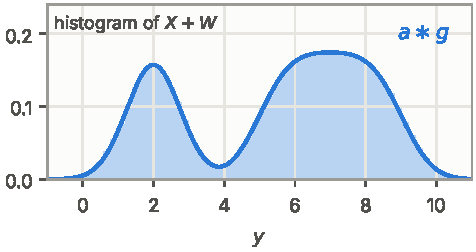
\includegraphics[width=\linewidth]{figures/ch02_conv_result.pdf}
\caption{The density of a sum, on the line. (a) $X$ has the density $a$:
with probability $0.3$ a Gaussian with mean $2$ and standard deviation
$0.3$ (the peak), with probability $0.7$ uniform on $[5,9]$ (the
plateau). (b) $W$, independent of $X$, has the density
$g=\Normal(0,0.7^2)$. (c) The sum $X+W$ has the density $a\ast g$. In
each panel, the histogram is that of $200\,000$ draws, and the curve is
the density.}
\label{fig:convresult}
\end{figure}

\begin{figure}[t]
\centering
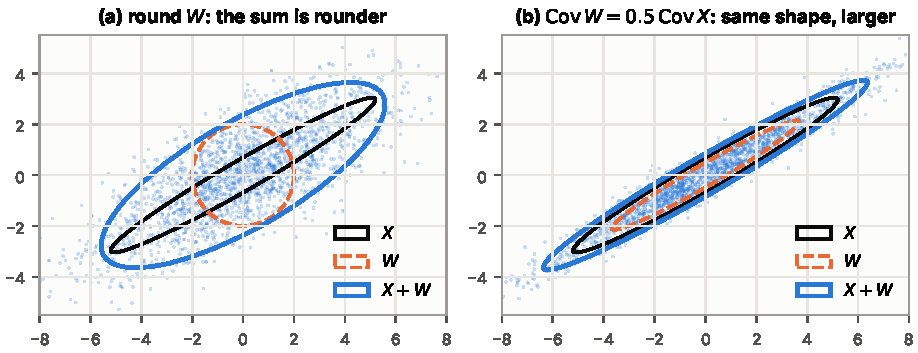
\includegraphics[width=0.85\linewidth]{figures/ch02_cov_sum.pdf}
\caption{The $2\sigma$ covariance ellipses of $X$ (black), of an
independent $W$ (orange, dashed) and of $X+W$ (blue), with $2\,000$
draws of $X+W$. $X$ has the standard deviations $3$ and $0.3$ along axes
turned by $30^\circ$. (a) A round $W$, $\Cov W=I$: the ellipse of $X+W$
contains that of $X$ and is rounder (axis ratio $3.0$ instead of $10$).
(b) $\Cov W=0.5\Cov X$: the ellipse of $X+W$ has the shape of that of
$X$, enlarged by $\sqrt{1.5}\approx1.22$.}
\label{fig:covsum}
\end{figure}

\begin{proposition}[unbreakable]{Prediction with a known heading is a convolution}{conv}
Suppose the heading $\psi_t$ during the drive is known (in the grid
filter, it is the compass reading) and the position moves by
$\p_{t+1}=\p_t+\vect{d}_t+\w_t$, with the displacement
$\vect{d}_t=s_t(\cos\psi_t,\sin\psi_t)$ and a noise
$\w_t\sim\Normal(\vect0,\Sigma_t)$ independent of $\p_t$. Then
\[
  \belbar(\p)=\bigl(\bel(\,\cdot-\vect{d}_t)\ast\Normal(\vect0,\Sigma_t)
  \bigr)(\p),
\]
the belief shifted by $\vect{d}_t$ and blurred by the noise density.
\end{proposition}

\begin{proof}
Write $g$ for the density of $\Normal(\vect0,\Sigma_t)$, and
$\bel(\,\cdot-\vect d_t)$ for the function
$\vect q\mapsto\bel(\vect q-\vect d_t)$: the belief \emph{shifted} by
$\vect d_t$. Its value at $\vect q$ is the old belief at
$\vect q-\vect d_t$, the point from which the displacement $\vect d_t$
leads to $\vect q$. There are two ways to the result. The first gives the
picture, the second checks it on the prediction formula
\eqref{eq:predict}.

\emph{First way: a sum of two independent vectors.} Group the terms as
$\p_{t+1}=(\p_t+\vect d_t)+\w_t$.
\begin{itemize}[nosep]
  \item $\p_t+\vect d_t$ is the old position moved by the known
        displacement, and its density is the shifted belief. For a region
        $B$, write $B-\vect d_t$ for the region $B$ moved by
        $-\vect d_t$. Then
        \[
          \Pr(\p_t+\vect d_t\in B)=\Pr(\p_t\in B-\vect d_t)
          =\int_{B-\vect d_t}\bel(\vect x)\,\mathrm d\vect x
          =\int_B\bel(\vect q-\vect d_t)\,\mathrm d\vect q ,
        \]
        with the change of variable $\vect q=\vect x+\vect d_t$, a
        translation, so $\mathrm d\vect x=\mathrm d\vect q$.
  \item $\w_t$ has the density $g$, and it is independent of $\p_t$,
        hence of $\p_t+\vect d_t$, since $\vect d_t$ is known.
  \item By the probabilistic meaning of the convolution, shown above,
        the sum $\p_{t+1}$ has the density
        $\bel(\,\cdot-\vect d_t)\ast g$.
\end{itemize}

\emph{Second way: from the prediction formula.} Given $\p_t$, the only
random term in $\p_{t+1}=\p_t+\vect d_t+\w_t$ is $\w_t$, and knowing
$\p_t$ does not change its distribution, since the two are independent.
So, given $\p_t$, $\p_{t+1}$ is Gaussian with the mean $\p_t+\vect d_t$
and the covariance $\Sigma_t$. A Gaussian density depends on the point
only through its difference with the mean, so
\[
  p(\p_{t+1}\mid\p_t)=\Normal(\p_{t+1};\,\p_t+\vect d_t,\,\Sigma_t)
  =g(\p_{t+1}-\p_t-\vect d_t).
\]
Call the new position $\p$ and the old one $\vect q$, and go line by
line from \eqref{eq:predict}:
\begin{align*}
  \belbar(\p)
  &=\int g(\p-\vect q-\vect d_t)\,\bel(\vect q)\,\mathrm d\vect q
  &&\text{\eqref{eq:predict} with this transition}\\
  &=\int g(\p-\vect q')\,\bel(\vect q'-\vect d_t)\,\mathrm d\vect q'
  &&\text{$\vect q'=\vect q+\vect d_t$, $\mathrm d\vect q=\mathrm d\vect q'$}\\
  &=\bigl(g\ast\bel(\,\cdot-\vect d_t)\bigr)(\p)
  &&\text{definition of the convolution}\\
  &=\bigl(\bel(\,\cdot-\vect d_t)\ast g\bigr)(\p)
  &&\text{the order does not matter.}
\end{align*}
In the third line, the definition $(a\ast g)(\p)=\int a(\p-\vect q)\,
g(\vect q)\,\mathrm d\vect q$ is used with the roles of the two functions
exchanged: $g$ is evaluated at $\p-\vect q'$, and the shifted belief at
$\vect q'$.
\end{proof}

The same position-only model, with its noise covariance $\Sigma_t$
worked out, is the one the Kalman filter will use in
\cref{sec:linmower}.

On the grid, the prediction of \cref{prop:conv} is done in two moves:
shift the table by $\vect d_t$, then blur it with a discrete Gaussian
filter. A grid cannot represent a blur narrower than a cell. Here the
motion noise has a standard deviation of about $0.4$ units, a tenth of a
cell 4 units wide, so the filter blurs by more than the noise, and the
predicted belief comes out a little wider than the noise warrants. This
costs nothing at this resolution, since the grid cannot place the robot
more precisely than a cell anyway. Notebook~01 shows the code of the
prediction and its exact choices, and prints these numbers.

The update \eqref{eq:update} multiplies the predicted density by the
likelihood and renormalises. On the grid, write $\bar b_i$ for the
predicted probability of the cell $C_i$, and integrate
\eqref{eq:update} over that cell:
\begin{align*}
  b_i&=\int_{C_i}\bel(\p)\,\mathrm d\p
  &&\text{probability of the cell}\\
  &=\eta\int_{C_i}p(\z\mid\p)\,\belbar(\p)\,\mathrm d\p
  &&\text{\eqref{eq:update}}\\
  &\approx\eta\,p(\z\mid\vect c_i)\int_{C_i}\belbar(\p)\,\mathrm d\p
  &&\text{likelihood taken at the centre}\\
  &=\eta\,p(\z\mid\vect c_i)\,\bar b_i
  &&\text{definition of }\bar b_i .
\end{align*}
The only approximation is the third line: across the cell, the
likelihood is replaced by its value at the centre, which is accurate when
it changes little over a cell. The constant $\eta$ follows from
$\sum_ib_i=1$: $\eta^{-1}=\sum_jp(\z\mid\vect c_j)\,\bar b_j$, the grid
version of the integral in \eqref{eq:update}. So the update is a product
cell by cell, followed by a division by the sum. In the code the new
table overwrites the old one, which is written
$b_i\leftarrow\eta\,p(\z\mid\vect c_i)\,b_i$, the $b_i$ on the right being
the predicted values.

\paragraph{A lawn of any shape.} Nothing in the grid filter needs a
square lawn. A lawn of any shape, with a tree or a flower bed in it, is
covered by the grid of a rectangle that contains it, and each cell is
marked as \emph{lawn} or \emph{not lawn}: the \emph{mask}
(\cref{fig:potato}, left). A cell cut by the edge can be marked by its
centre, or weighted by the fraction of its area on the lawn. The filter
then does three things: it starts with a belief spread over the lawn
cells only; after each prediction it sets the belief of the other cells
to zero and renormalises (\cref{fig:potato}, right); and it updates as
before. The step after the prediction is an update in disguise. Knowing
that the robot is on the lawn is an observation whose likelihood is $1$
on the lawn and $0$ elsewhere, and multiplying by it and renormalising is
Bayes' rule. It is correct as long as the robot cannot leave the lawn,
which a real mower guarantees by a boundary wire or by a geofence (see
the box below). Near
the edge, the convolution of \cref{prop:conv} is therefore no longer the
whole prediction: the blur puts probability where the robot cannot be,
and the mask removes it. Away from the edge it is exact, as before. The
square lawn of the simulations is the simplest case of this: there, the
probability that leaves the lawn is the part outside a square.

\begin{figure}[t]
\centering
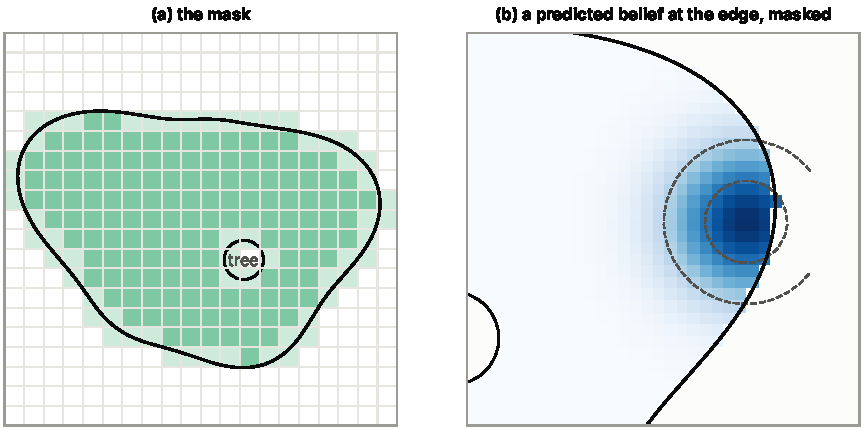
\includegraphics[width=\linewidth]{figures/ch02_potato.pdf}
\caption{A potato-shaped lawn with a tree. Left: the mask on a grid of
16-unit cells (the filter uses 4-unit cells): cells entirely on the lawn
(dark), cells cut by the edge or by the tree (light), the others (white).
Right: a predicted belief next to the edge, with 4-unit cells. The dashed
circles are the levels of the Gaussian blur; the $27\%$ of it that falls
off the lawn is set to zero, and the rest is renormalised.}
\label{fig:potato}
\end{figure}

\begin{mower}
\textbf{Boundary wire or geofence.} A \emph{boundary wire} is buried
along the edge, and the mower senses it directly: it turns back when it
reaches the wire, whatever it believes about its position. A
\emph{geofence} is a virtual boundary in software: the edge is recorded
once, by walking or driving around the lawn with the RTK GPS, and the
controller stops the robot, or turns it back, when its position comes
too close to that edge. The same recorded edge then serves twice: as the
geofence for the controller and as the mask for the filter. But a
geofence is enforced with the \emph{estimated} position, so it is only
as good as the localisation. With an RTK fix the position is good to a
few centimetres and the geofence is as good as a wall. Under trees, next
to the house, or when the correction link drops, the fix degrades and
the error can grow to metres: the robot could cross the real edge while
it believes it is inside. So the controller keeps a margin from the edge
that grows with the uncertainty of the filter (a few of its standard
deviations), or stops when the fix is lost. The assumption of the mask,
``the robot never leaves the lawn'', holds for a geofenced mower only as
long as that margin is kept; a wire does not have this weakness, which is
one reason why some mowers keep one even with an RTK GPS.
\end{mower}

On a real robot this mask is the \emph{map}. Robot navigation software
stores it as an \emph{occupancy grid}, whose cells are free, occupied or
unknown, and Monte Carlo localisation gives zero weight to particles in
occupied cells; the particle filter of \cref{ch:particle} gives zero
likelihood to particles more than 5 units off the lawn. For a mower with an RTK GPS, walking once around the lawn
records its edge, and the mask follows.

\section{Two bumps}
\label{sec:twobumps}

We make the problem hard on purpose: the robot measures only
\emph{ranges}, and only to two landmarks. A range to a landmark places
the robot on a circle around it; two ranges place it on two circles, which
meet in two points (\cref{fig:mirror}). The two points are mirror images
of each other across the line through the landmarks, and no range
measurement can tell them apart.

\begin{figure}[ht]
\centering
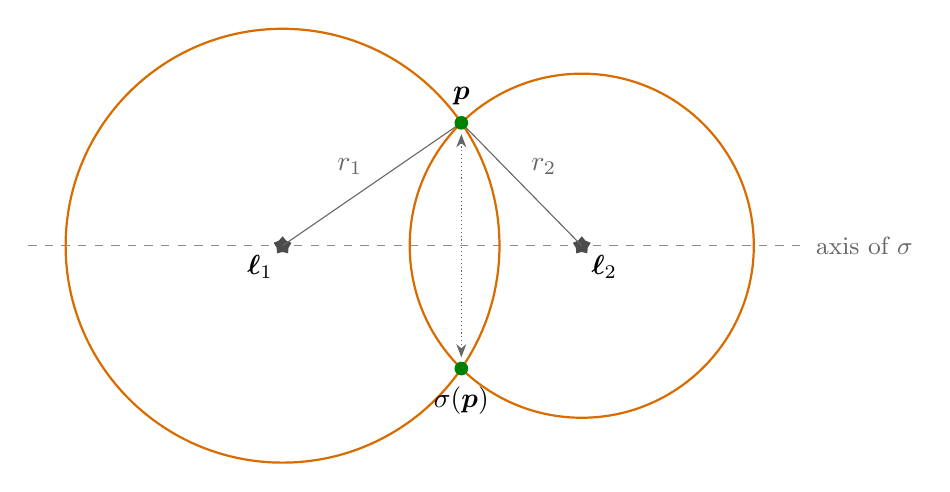
\begin{tikzpicture}[scale=0.95,>=Stealth]
  \coordinate (A) at (0,0);
  \coordinate (B) at (4,0);
  \def\ra{2.9}\def\rb{2.3}
  % intersection: x = (ra^2 - rb^2 + d^2)/(2d), y = sqrt(ra^2 - x^2)
  \pgfmathsetmacro{\xi}{(\ra*\ra-\rb*\rb+16)/8}
  \pgfmathsetmacro{\yi}{sqrt(\ra*\ra-\xi*\xi)}
  \draw[dashed,black!45] (-3.4,0) -- (7.0,0) node[right,black!60]
    {\small axis of $\sigma$};
  \draw[orange!85!black,thick] (A) circle (\ra);
  \draw[orange!85!black,thick] (B) circle (\rb);
  \node[star,star points=5,fill=black!70,inner sep=1.6pt] at (A) {};
  \node[star,star points=5,fill=black!70,inner sep=1.6pt] at (B) {};
  \node[below left] at (A) {$\bell_1$};
  \node[below right] at (B) {$\bell_2$};
  \draw[black!60] (A) -- (\xi,\yi) node[pos=0.5,above left] {$r_1$};
  \draw[black!60] (B) -- (\xi,\yi) node[pos=0.5,above right] {$r_2$};
  \fill[green!50!black] (\xi,\yi) circle (2.6pt)
    node[above=3pt,black] {$\p$};
  \fill[green!50!black] (\xi,-\yi) circle (2.6pt)
    node[below=3pt,black] {$\sigma(\p)$};
  \draw[<->,densely dotted,black!60] (\xi,\yi-0.15) -- (\xi,-\yi+0.15);
\end{tikzpicture}
\caption{Two ranges $r_1$, $r_2$ to two landmarks define two circles,
which meet at $\p$ and at its mirror image $\sigma(\p)$ across the line
through the landmarks. The two points have exactly the same ranges.}
\label{fig:mirror}
\end{figure}

\begin{proposition}{Mirror ambiguity}{mirror}
Let $\sigma$ be the reflection across the line through $\bell_1$ and
$\bell_2$. Then $\norm{\bell_j-\sigma(\p)}=\norm{\bell_j-\p}$ for $j=1,2$
and every $\p$. Consequently, if the belief before a range-only update is
\emph{invariant under $\sigma$}, meaning that it has the same value at
$\p$ and at $\sigma(\p)$ for every $\p$, the belief after the update is
also invariant under $\sigma$.
\end{proposition}

\begin{proof}
A reflection is an isometry, and it fixes every point of its axis, in
particular $\bell_1$ and $\bell_2$. So
$\norm{\bell_j-\sigma(\p)}=\norm{\sigma(\bell_j)-\sigma(\p)}=
\norm{\bell_j-\p}$. The likelihood of two ranges depends on the position
only through its two distances to the landmarks, so it is the same at
$\p$ and $\sigma(\p)$. The update multiplies a $\sigma$-invariant
belief by this $\sigma$-invariant likelihood, and a product of two
functions that are each the same at $\p$ and $\sigma(\p)$ is again the
same at $\p$ and $\sigma(\p)$.
\end{proof}

\begin{figure}[ht]
\centering
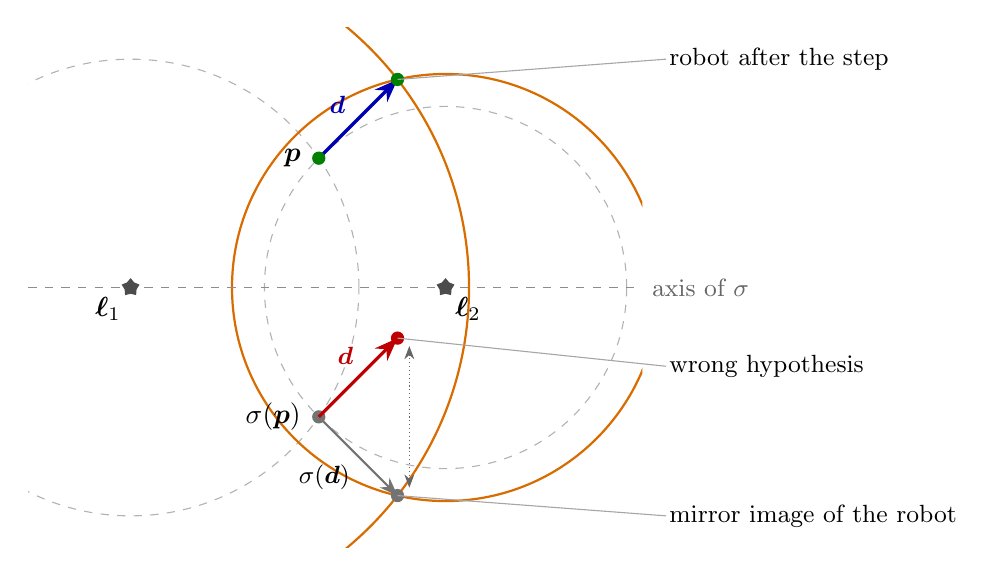
\begin{tikzpicture}[scale=1.0,>=Stealth,
    lab/.style={font=\small,anchor=west,inner sep=1pt,text=black},
    lead/.style={black!35,thin}]
  \coordinate (A) at (0,0);
  \coordinate (B) at (4,0);
  \def\ra{2.9}\def\rb{2.3}\def\dx{1.0}\def\dy{1.0}
  % the robot before the step: the intersection of the old circles (as in Fig. 2.7)
  \pgfmathsetmacro{\xi}{(\ra*\ra-\rb*\rb+16)/8}
  \pgfmathsetmacro{\yi}{sqrt(\ra*\ra-\xi*\xi)}
  % the robot after the step, and its new ranges
  \pgfmathsetmacro{\xn}{\xi+\dx}
  \pgfmathsetmacro{\yn}{\yi+\dy}
  \pgfmathsetmacro{\rna}{sqrt(\xn*\xn+\yn*\yn)}
  \pgfmathsetmacro{\rnb}{sqrt((\xn-4)*(\xn-4)+\yn*\yn)}
  \begin{scope}
    \clip (-1.3,-3.3) rectangle (6.5,3.3);
    \draw[dashed,black!30] (A) circle (\ra);
    \draw[dashed,black!30] (B) circle (\rb);
    \draw[orange!85!black,thick] (A) circle (\rna);
    \draw[orange!85!black,thick] (B) circle (\rnb);
  \end{scope}
  \draw[dashed,black!45] (-1.3,0) -- (6.5,0) node[right,black!60]
    {\small axis of $\sigma$};
  \node[star,star points=5,fill=black!70,inner sep=1.6pt] at (A) {};
  \node[star,star points=5,fill=black!70,inner sep=1.6pt] at (B) {};
  \node[below left] at (A) {$\bell_1$};
  \node[below right] at (B) {$\bell_2$};
  % the robot moves by d
  \draw[->,very thick,blue!70!black] (\xi,\yi) -- (\xn,\yn)
    node[pos=0.45,above left=-1pt,font=\small] {$\vect d$};
  \fill[green!50!black] (\xi,\yi) circle (2.4pt) node[left=3pt,black] {$\p$};
  \fill[green!50!black] (\xn,\yn) circle (2.4pt);
  \draw[lead] (\xn,\yn) -- (6.8,2.9) node[lab] {robot after the step};
  % its mirror image moves by sigma(d)
  \draw[->,thick,black!55] (\xi,-\yi) -- (\xn,-\yn)
    node[pos=0.5,below left=-1pt,font=\small,black] {$\sigma(\vect d)$};
  \fill[black!55] (\xi,-\yi) circle (2.4pt) node[left=3pt,black] {$\sigma(\p)$};
  \fill[black!55] (\xn,-\yn) circle (2.4pt);
  \draw[lead] (\xn,-\yn) -- (6.8,-2.9) node[lab] {mirror image of the robot};
  % the wrong hypothesis is moved by d
  \draw[->,very thick,red!75!black] (\xi,-\yi) -- (\xi+\dx,-\yi+\dy)
    node[pos=0.55,above left=-1pt,font=\small] {$\vect d$};
  \fill[red!75!black] (\xi+\dx,-\yi+\dy) circle (2.4pt);
  \draw[lead] (\xi+\dx,-\yi+\dy) -- (6.8,-1.0) node[lab] {wrong hypothesis};
  \draw[<->,densely dotted,black!60] (\xn+0.15,-\yi+\dy-0.1) --
    (\xn+0.15,-\yn+0.1);
\end{tikzpicture}
\caption{Why motion breaks the tie, with the two landmarks of
\cref{fig:mirror}. Before the step, the ranges give two circles (dashed)
that meet at the robot $\p$ and at its mirror image $\sigma(\p)$. The
robot moves by $\vect d$ (blue). The new ranges give two new circles
(orange), which meet at the new position and at its mirror image, reached
from $\sigma(\p)$ by the mirrored displacement $\sigma(\vect d)$ (grey).
The filter knows the heading and moves every hypothesis by the same
$\vect d$, also the one at $\sigma(\p)$ (red). That wrong hypothesis is
not at an intersection of the new circles (dotted gap): its ranges no
longer agree with the measurements.}
\label{fig:mirrormotion}
\end{figure}

What can tell the two points apart is the \emph{motion}, and the
likelihood then does the work. Look at one cycle of the filter, starting
from a belief with two mirror bumps.

\emph{Prediction: the motion breaks the symmetry.} The heading is known,
so the filter moves the whole belief, both bumps, by the same
displacement $\vect d$. The robot moves by $\vect d$, but its mirror
image moves by the mirrored displacement $\sigma(\vect d)$ (for a
displacement, the reflection of the vector, without translation). So the
wrong bump ends up at $\sigma(\p)+\vect d$, while the mirror image of the
robot is at $\sigma(\p)+\sigma(\vect d)$. The gap between them is
$\vect d-\sigma(\vect d)$, twice the part of $\vect d$ perpendicular to
the axis; it vanishes only when $\vect d$ is parallel to the axis. The
prediction removes no probability: it only moves the wrong bump to a
place where the ranges will not match.

\emph{Update: the likelihood removes the wrong bump.} The likelihood of
the new ranges is $\sigma$-invariant (\cref{prop:mirror}). It is large
near the two intersections of the new circles: the robot and its mirror
image (\cref{fig:mirrormotion}). The right bump sits at one of them; the
wrong bump sits away from both, because two points have the same
distances to two distinct landmarks only if they are equal or mirror
images (two circles with distinct centres meet in at most two points). So
the update multiplies the wrong bump by a smaller value than the right
one, and after renormalisation the wrong bump has lost mass to the right
one.

Neither step works alone. Without motion, or with a motion parallel to
the axis, the belief stays $\sigma$-invariant and, by
\cref{prop:mirror}, every update keeps the two bumps as they are. Without
the likelihood, the prediction only moves and blurs the bumps.

\emph{Why it takes several steps.} Write $\rho_j(\vect x)=
\norm{\bell_j-\vect x}$ for the distance from a point $\vect x$ to the
landmark $\bell_j$. The measured range is $z_j=\rho_j(\p)+v_j$, with a
noise $v_j\sim\Normal(0,\sigma_r^2)$, $\sigma_r=5$. Call $\vect w$ the
position of the wrong bump, and $e_j=\rho_j(\vect w)-\rho_j(\p)$ its
\emph{range errors}.

First, the update acts on the ratio of the two masses through the ratio
of the likelihoods. Treat each bump as if its mass were at one point: $m_{\vect w}$
at $\vect w$ and $m_{\p}$ at $\p$ before the update. The update
\eqref{eq:update} multiplies each mass by the likelihood at its point and
by the same constant $\eta$, so after the update
\[
  \frac{\eta\,p(\z\mid\vect w)\,m_{\vect w}}{\eta\,p(\z\mid\p)\,m_{\p}}
  =\frac{p(\z\mid\vect w)}{p(\z\mid\p)}\cdot\frac{m_{\vect w}}{m_{\p}} :
\]
$\eta$ cancels, and the ratio of the masses is multiplied by the ratio of
the likelihoods.

Next, that ratio. The two ranges have independent Gaussian noises, so the
likelihood at a point $\vect x$ is
$p(\z\mid\vect x)=C\prod_je^{-(z_j-\rho_j(\vect x))^2/(2\sigma_r^2)}$,
with a constant $C$ that does not depend on $\vect x$. At the robot,
$z_j-\rho_j(\p)=v_j$. At the wrong bump,
$z_j-\rho_j(\vect w)=\bigl(z_j-\rho_j(\p)\bigr)-\bigl(\rho_j(\vect w)
-\rho_j(\p)\bigr)=v_j-e_j$. Then, line by line:
\begin{align*}
  \frac{p(\z\mid\vect w)}{p(\z\mid\p)}
  &=\frac{C\prod_je^{-(v_j-e_j)^2/(2\sigma_r^2)}}
         {C\prod_je^{-v_j^2/(2\sigma_r^2)}}
  &&\text{the two likelihoods}\\
  &=\prod_j\exp\Bigl(-\frac{(v_j-e_j)^2-v_j^2}{2\sigma_r^2}\Bigr)
  &&\text{$C$ cancels; $e^a/e^b=e^{a-b}$, factor by factor}\\
  &=\prod_j\exp\Bigl(-\frac{e_j^2-2e_jv_j}{2\sigma_r^2}\Bigr)
  &&(v_j-e_j)^2=v_j^2-2e_jv_j+e_j^2\\
  &=\exp\Bigl(-\sum_j\frac{e_j^2}{2\sigma_r^2}
   +\sum_j\frac{e_jv_j}{\sigma_r^2}\Bigr)
  &&\textstyle\prod_je^{a_j}=e^{\sum_ja_j}.
\end{align*}
In the exponent, the first term always favours
the right bump, and it grows like the \emph{square} of the range errors.
The second is random: the noises $v_j$ are independent, with mean $0$
and variance $\sigma_r^2$, so it has the mean $0$ and the variance
$\sum_je_j^2\sigma_r^2/\sigma_r^4=\sum_je_j^2/\sigma_r^2$, that is the
standard deviation $\sqrt{\sum_je_j^2}/\sigma_r$: it grows only like the
errors themselves.
While the range errors are smaller than $\sigma_r$, both terms are small,
and the second can favour either bump. Once they are larger than
$\sigma_r$, the first term wins, and the wrong bump loses most of its mass
at every update. The range errors grow with the gap, so the filter needs
a few steps of driving before the ranges can separate the two bumps.

\begin{figure}[ht]
\centering
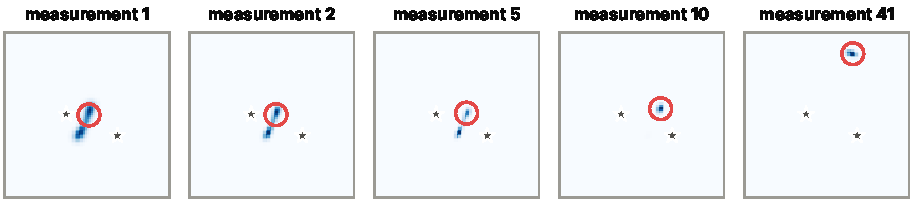
\includegraphics[width=\linewidth]{figures/ch02_grid_bimodal.pdf}
\caption{Grid belief (darker is more probable; a power-law colour scale
makes small masses visible) with range-only sensing to two landmarks
(stars); the red circle surrounds the true position. The first measurement gives a
belief symmetric about the line through the landmarks (nearly: the
uniform start is cut off by the edges of the lawn, which are not symmetric
about that line): two bumps. Both survive for a few measurements, and at
measurements 4 and 5 the \emph{wrong} one carries more mass than the right
one (at measurement 5, $0.65$ against $0.35$ on the two sides of the
line; notebook~01 prints these masses for the first ten measurements). As
the robot drives on, the wrong bump stops agreeing with the ranges: by
measurement 8 it has disappeared, and the belief then follows the robot.}
\label{fig:gridbimodal}
\end{figure}

The run of \cref{fig:gridbimodal} has only the first two landmarks
(seed 1) and starts from a uniform belief over the lawn. The table
follows the \emph{wrong track}: the mirror image of the robot at
measurement 1, moved afterwards by the robot's own displacements. For
each measurement $k$ it gives the gap to the mirror image of the robot,
the range errors $e_1,e_2$ of the wrong track, the range noises
$v_1,v_2$, the factor by which the update multiplied the ratio (mass on
the wrong side)\,/\,(mass on the right side) of the grid, and the mass on
the wrong side after the update (notebook~01 prints all of them).
\begin{center}
\small
\begin{tabular}{@{}rrrrrrrr@{}}
\toprule
$k$ & gap & $e_1$ & $e_2$ & $v_1$ & $v_2$ & update factor &
mass on the wrong side\\
\midrule
 1 &  0.0 &   0.0 &   0.0 &  1.7 &  4.5 & ---  & 0.50\\
 2 &  4.3 &  $-$1.4 &  $-$1.0 &  2.7 & $-$0.8 & 1.09 & 0.51\\
 3 &  8.5 &  $-$2.7 &  $-$2.2 &  0.0 &  6.5 & 0.80 & 0.44\\
 4 & 13.2 &  $-$3.9 &  $-$3.5 &  1.1 & $-$5.6 & 1.70 & 0.57\\
 5 & 18.0 &  $-$5.0 &  $-$5.0 &  0.8 & $-$6.1 & 1.44 & 0.65\\
 6 & 23.5 &  $-$6.2 &  $-$6.8 & $-$2.5 &  4.5 & 0.35 & 0.39\\
 7 & 29.6 &  $-$7.4 &  $-$8.9 &  4.6 & $-$6.2 & 0.45 & 0.22\\
 8 & 35.0 &  $-$8.3 & $-$10.8 & $-$2.3 &  3.8 & 0.06 & 0.01\\
 9 & 40.9 &  $-$9.3 & $-$12.9 &  1.3 & $-$1.7 & 0.05 & 0.00\\
10 & 47.5 & $-$10.4 & $-$15.2 & $-$6.0 &  3.4 & 0.02 & 0.00\\
\bottomrule
\end{tabular}
\end{center}
Three phases appear.
\begin{itemize}[nosep]
  \item \emph{Measurement 1.} The first update turns the uniform belief
        into two mirror bumps, with half of the mass each.
  \item \emph{Measurements 2 to 5.} The gap grows by about $4$ to $5$
        units per step, but the range errors stay at or below
        $\sigma_r=5$, so the update factors are close to $1$ and the
        noise decides their direction. At measurements 4 and 5 it
        favours the wrong bump: the measured range to $\bell_2$ was short
        by $5.6$ and $6.1$, and the wrong track is also closer to
        $\bell_2$ than the robot ($e_2=-3.5$ and $-5.0$), so its ranges
        fit the measurements better. The wrong side then carries $0.65$ of
        the mass.
  \item \emph{Measurements 6 to 10.} The range errors exceed $\sigma_r$,
        the first term wins, and the factors drop to $0.35$, $0.45$,
        then about $0.05$ and below: the wrong bump is gone by
        measurement 8.
\end{itemize}
For the bumps as a whole the factors are not exactly the ratio of the
likelihoods at two points, because each bump is spread over many cells,
but they follow the same pattern.

\begin{inwords}
The true posterior can have several separate bumps, and the right bump
need not be the biggest one for a while. A filter that represents only
one bump, or that commits early to the most probable one, could have
chosen the mirror image at measurement 4 or 5, with no way back. A Gaussian
belief is worse still: its mean would sit \emph{between} the two bumps,
where the robot certainly is not.
\end{inwords}

\section{The cost of a grid}

The grid is exact up to discretisation and can represent any belief. Its
cost is the number of cells, and every step touches every cell. If the
state has $d$ coordinates and each is cut into $n$ intervals, the grid has
$n^d$ cells. With $n=80$: $6\,400$ cells for the position, about half a million for the
pose $(x,y,\theta)$ (the classic \emph{Markov localisation} of the 1990s,
feasible), $2.6\times10^{11}$ for a pose with its three velocities (six
dimensions). And at any
time, almost all of those cells have negligible probability. There are two
ways out, and the rest of the book follows both:
\begin{enumerate}[nosep]
\item \emph{assume a shape} for the belief, a Gaussian described by a mean
  and a covariance ($d+d(d+1)/2$ numbers): the Kalman family,
  Part~II;
\item \emph{sample} the belief, putting the computation only where the
  probability is: the particle filter, Chapter~\ref{ch:particle}.
\end{enumerate}

\begin{practice}[\nb{01\_bayes\_filter.ipynb}, \code{grid.py}]
\code{GridFilter} implements the predict and update steps above on cells
4 units wide ($80\times80$ cells), with \code{sensor="range"} or \code{"range\_bearing"}. The notebook
reproduces \cref{fig:gridbimodal} and compares the grid filter with dead
reckoning: with two noisy ranges per step, its median error after step 20
is $2.3$, less than half the range noise $\sigma_r=5$, although the cells are
4~units wide. Things to try:
switch to range--bearing (a bearing tells the side of the axis and the
ambiguity disappears), use all four landmarks, or enlarge the cells.
\end{practice}

\begin{mower}
A mower that wakes up in the morning does not know where it was left. The
first measurements are rarely enough to pin it down, especially with
symmetric landmark layouts (four beacons at the corners of a rectangular
lawn are symmetric under a half-turn) or with only ranges, as with radio
beacons. The ambiguity is real, and a localisation system must be able to
carry several hypotheses until the motion resolves them.
\end{mower}

\section*{What to remember from this chapter}
\addcontentsline{toc}{section}{What to remember}

\begin{enumerate}[nosep]
  \item The belief $\bel(\x_t)$ is the distribution of the current pose
    given all controls and measurements so far. It is the complete answer
    to ``where is the robot?''.
  \item The Bayes filter updates it in two steps. \emph{Predict}
    \eqref{eq:predict}: push the belief through the motion model; it
    blurs. \emph{Update} \eqref{eq:update}: multiply by the likelihood of
    the new measurement and renormalise; it sharpens.
  \item The normaliser $\eta^{-1}$ is the value of the density that the
    filter gave to the measurement before seeing it: a measure of
    surprise.
  \item The exact belief can have several bumps, and the right one is not
    always the biggest.
  \item A grid computes the recursion with no assumption on the shape of
    the belief, but its cost grows exponentially with the dimension of the
    state. Every other filter of the book is a cheaper approximation of
    the same recursion.
\end{enumerate}

\FloatBarrier
\section*{Exercises}
\addcontentsline{toc}{section}{Exercises}

\begin{enumerate}[label=\textbf{2.\arabic*},ref=2.\arabic*]
\item\label{ex:twostate} \emph{A two-state filter.} In the setting of
  \cref{ex:grassgravel}, start from $\bel=(0.5,0.5)$ and compute the belief
  after the readings ``rough'', ``rough''.
\item\label{ex:blur} Show that blurring with $\Normal(\vect0,\Sigma_1)$ and
  then with $\Normal(\vect0,\Sigma_2)$ is the same as blurring once with
  $\Normal(\vect0,\Sigma_1+\Sigma_2)$. What does it say about the width of
  a grid belief after $t$ predictions without updates?
\item\label{ex:nomotion} Suppose the robot is parked (so the prediction is
  the identity) and keeps receiving range-only readings from the same two
  landmarks. Show that the belief stays bimodal forever, and that each bump
  keeps probability $1/2$ if the prior was symmetric.
\item\label{ex:gridcost} A robot localises on a $30\times30$\,m lawn with a
  pose grid of $5$\,cm and $1^\circ$. How many cells is that, and how many
  bytes in single precision? How many floating-point operations does one
  prediction cost if it is done as a full sum over pairs of cells?
\item\label{ex:potato} \emph{A potato-shaped lawn.} The lawn of
  \cref{fig:potato} has a curved edge and a tree.
  \begin{enumerate}[nosep]
    \item Show that setting the belief of the cells off the lawn to zero
          and renormalising is Bayes' rule for an observation ``the
          robot is on the lawn''. What is its likelihood?
    \item Why is the convolution of \cref{prop:conv} still the exact
          prediction far from the edge, but not next to it? What does the
          masking assume about the robot?
    \item The lawn fits in a $320\times320$ square. With 4-unit cells,
          $2749$ of the $6400$ cells of the square have their centre on
          the lawn. How can the filter avoid storing and updating the
          others?
  \end{enumerate}
\end{enumerate}

\subsection*{Solutions}

\solution{2.1} Each step is a prediction followed by an update, as in
\cref{ex:grassgravel}: the robot may change surface between two readings.
Order the states as $(G,P)$; the sensor says ``rough'' with probability
$0.3$ on the grass and $0.8$ on the path.

\emph{First step.} Predict: $\belbar(G)=0.9\times0.5+0.1\times0.5=0.5$,
and likewise $\belbar(P)=0.5$. The belief $(0.5,0.5)$ does not change: as
much probability flows from the grass to the path as back. Update with
``rough'': multiply each predicted probability by the probability of the
reading in that state, add, and divide by the sum.
\begin{center}
\begin{tabular}{lccc}
  \toprule
  & predicted & $\times\,p(\text{rough}\mid\cdot)$ & new belief\\
  \midrule
  grass & $0.5$ & $0.5\times0.3=0.15$ & $0.15/0.55=0.273$\\
  path  & $0.5$ & $0.5\times0.8=0.40$ & $0.40/0.55=0.727$\\
  \midrule
  total & $1$ & $0.55$ & $1$\\
  \bottomrule
\end{tabular}
\end{center}
The sum $0.55$ is the probability that the filter gave to the reading
``rough'' before seeing it.

\emph{Second step.} Predict: the robot is on the grass if it was there and
stayed, or on the path and left it:
\[
  \belbar(G)=0.9\times0.273+0.1\times0.727=0.318,\qquad
  \belbar(P)=0.1\times0.273+0.9\times0.727=0.682 .
\]
Update with ``rough'':
\begin{center}
\begin{tabular}{lccc}
  \toprule
  & predicted & $\times\,p(\text{rough}\mid\cdot)$ & new belief\\
  \midrule
  grass & $0.318$ & $0.318\times0.3=0.0955$ & $0.0955/0.641=0.149$\\
  path  & $0.682$ & $0.682\times0.8=0.5455$ & $0.5455/0.641=0.851$\\
  \midrule
  total & $1$ & $0.641$ & $1$\\
  \bottomrule
\end{tabular}
\end{center}
The belief after the two readings is $(0.149,\,0.851)$.

\emph{What the prediction did.} Without the prediction between the two
readings, that is if the robot could not change surface, the two readings
would multiply $(0.5,0.5)$ by $0.3\times0.3=0.09$ and $0.8\times0.8=0.64$,
which gives $(0.09,0.64)/0.73=(0.123,\,0.877)$. The filter is less sure
of the path, $0.851$ instead of $0.877$: between the readings, the
prediction moved $0.1\times0.727=0.073$ of probability from the path to
the grass, and only $0.1\times0.273=0.027$ back. A reading taken
\emph{before} a possible change of surface says less about the surface
\emph{after} it.

\solution{2.2} The idea: blurring a density with a Gaussian is adding an
independent Gaussian noise to a random vector that has this density, and
two independent Gaussian noises add up to one.

\emph{Step 1: a blur is an added noise.} Let $X$ have the density $b$, and
let $X_1\sim\Normal(\vect0,\Sigma_1)$ be independent of $X$, with the
density $g_1$. By the probabilistic meaning of the convolution
(\cref{sec:grid}), $b\ast g_1$ is the density of $X+X_1$.

\emph{Step 2: the second blur.} Let $X_2\sim\Normal(\vect0,\Sigma_2)$,
with the density $g_2$, be independent of $(X,X_1)$, hence of $X+X_1$. By
the same result, $(b\ast g_1)\ast g_2$ is the density of $(X+X_1)+X_2$.

\emph{Step 3: the two noises are one.} Group the terms the other way:
$(X+X_1)+X_2=X+(X_1+X_2)$. The sum $X_1+X_2$ is Gaussian, as a sum of two
independent Gaussians (\cref{lem:affine}, in \cref{ch:kalman}); its mean
is $\vect0$, and its covariance is $\Sigma_1+\Sigma_2$, because the
covariances of independent vectors add (\cref{sec:grid}). It is
independent of $X$, since $X_1$ and $X_2$ are. So, by Step~1 again, the
density of $X+(X_1+X_2)$ is $b\ast g_{12}$, with $g_{12}$ the density of
$\Normal(\vect0,\Sigma_1+\Sigma_2)$.

\emph{Conclusion.} Steps 2 and 3 give the density of the same random
vector, so $(b\ast g_1)\ast g_2=b\ast g_{12}$: two blurs are one blur with
the summed covariance.

\emph{After $t$ predictions without update.} Each prediction shifts the
belief and blurs it with $\Normal(\vect0,\Sigma)$ (\cref{prop:conv}). The
shifts only move the belief. Applying the result $t-1$ times, the $t$
blurs are one blur with $\Normal(\vect0,t\Sigma)$. Along a direction
$\vect u$, the standard deviation of that blur is
$\sqrt{t\,\vect u\T\Sigma\vect u}=\sqrt t\,\sqrt{\vect u\T\Sigma\vect u}$:
the width of the belief grows like $\sqrt t$. On the grid of
\cref{sec:grid}, each blur has the standard deviation $1.2$ units (the
floor of $0.3$ cell, notebook~01), so after $t$ predictions the blur alone
has the standard deviation $1.2\sqrt t$: for example $12$ units, three
cells, after $100$ predictions. This assumes a known heading, as in
\cref{prop:conv}. When the heading itself is uncertain, its errors
accumulate and turn into sideways errors that grow faster: on a straight
path the variance of the lateral error grows like $t^3$
(\cref{prop:deadreckoning}), so its standard deviation grows like
$t^{3/2}$.

\solution{2.3} There are two claims: the two bumps keep equal masses, and
the belief stays made of two bumps, which become narrower.

\emph{The belief after $k$ readings.} The prediction is the identity, so
each step only multiplies the belief by the likelihood of the new
readings $\z_i$ and renormalises. After $k$ steps, collecting the
constants into one,
\[
  \bel_k(\p)=\eta\,\bel_0(\p)\prod_{i=1}^kp(\z_i\mid\p).
\]

\emph{Equal masses.} By \cref{prop:mirror}, each likelihood is
$\sigma$-invariant: $p(\z_i\mid\sigma(\p))=p(\z_i\mid\p)$. If the prior is
$\sigma$-invariant too, every factor of the product takes the same value
at $\p$ and at $\sigma(\p)$, so $\bel_k(\sigma(\p))=\bel_k(\p)$ for every
$k$. The reflection maps the half-plane on one side of the axis onto the
other half-plane and keeps areas, so the two half-planes have the same
mass. The axis itself has zero area, so each half-plane has the mass
$1/2$, exactly, at every step, not only in the limit. If the prior is not
symmetric, the same argument shows that the ratio
$\bel_k(\sigma(\p))/\bel_k(\p)=\bel_0(\sigma(\p))/\bel_0(\p)$ never
changes: the readings cannot correct an asymmetry of the prior either.

\emph{Two narrowing bumps.} Take one landmark $\bell$, at the distance
$\rho(\p)=\norm{\bell-\p}$ from $\p$, and its $k$ readings
$r_1,\dots,r_k$, with independent noises $\Normal(0,\sigma_r^2)$. Write
$\bar r=\frac1k\sum_ir_i$ for their mean. The product of their
likelihoods is
\[
  \prod_{i=1}^ke^{-(r_i-\rho(\p))^2/(2\sigma_r^2)}
  =\exp\Bigl(-\frac{1}{2\sigma_r^2}\sum_{i=1}^k\bigl(r_i-\rho(\p)\bigr)^2\Bigr).
\]
Write $r_i-\rho=(r_i-\bar r)+(\bar r-\rho)$ and expand the square:
\[
  \sum_i(r_i-\rho)^2
  =\sum_i(r_i-\bar r)^2+2(\bar r-\rho)\sum_i(r_i-\bar r)+k(\bar r-\rho)^2
  =\sum_i(r_i-\bar r)^2+k(\bar r-\rho)^2 ,
\]
because $\sum_i(r_i-\bar r)=\sum_ir_i-k\bar r=0$. The first sum does not
contain $\p$, so
\[
  \prod_{i=1}^ke^{-(r_i-\rho(\p))^2/(2\sigma_r^2)}
  =C\,\exp\Bigl(-\frac{(\bar r-\rho(\p))^2}{2\,\sigma_r^2/k}\Bigr),
\]
with a constant $C$. This is the likelihood of a single reading $\bar r$
with the standard deviation $\sigma_r/\sqrt k$. The positions that agree
with the readings of this landmark form a ring around it, of radius about
$\bar r$ and width proportional to $\sigma_r/\sqrt k$. The two rings, one
per landmark, meet in two spots around $\p$ and $\sigma(\p)$, which shrink
like $1/\sqrt k$. Only a motion that is not parallel to the axis, or a
third landmark off the axis, can break the tie (\cref{sec:twobumps}).

\solution{2.4} \emph{Cells.} Along each side, $30\,\text{m}/5\,\text{cm}
=600$ cells; for the heading, $360$ cells of $1^\circ$. In total
$600\times600\times360=129\,600\,000\approx1.3\times10^8$ cells.

\emph{Memory.} In single precision a number takes $4$ bytes, so the
belief takes $4\times1.3\times10^8\approx5.2\times10^8$ bytes, about
$520$\,MB.

\emph{A prediction as a full sum.} Write the prediction
\eqref{eq:predict} on the cells as $\bar b_i=\sum_jT_{ij}b_j$, with
$T_{ij}$ the probability of going from the cell $j$ to the cell $i$. Each
of the $n\approx1.3\times10^8$ new values is a sum of $n$ products, so the
prediction costs $n^2\approx1.7\times10^{16}$ multiplications and as many
additions. At $10^{10}$ operations per second, a fast processor, that is
$3.4\times10^6$ seconds, about $39$ days, for one prediction. The matrix
$T$ itself, with $n^2$ entries, would not fit in any memory.

\emph{Using the structure.} The probability of going from $j$ to $i$ is
negligible unless $i$ is near the cell reached from $j$ by the commanded
motion: the prediction is a shift and a local blur (\cref{prop:conv}).
A Gaussian blur over $5$ cells along each of the three axes, done one
axis at a time, costs $3\times5=15$ multiplications per cell, about
$2\times10^9$ per prediction: a fraction of a second. So the grid filters
that work in practice are built on such shifts and blurs, or on sparse
transitions. Even then, $520$\,MB of belief updated several times per
second is a lot for an embedded computer.

\solution{2.5}
\begin{enumerate}[nosep]
  \item Let $L$ be the set of the lawn cells, and take as observation
        the statement ``the robot is on the lawn''. Its likelihood in the
        cell $C_i$ is the probability of that statement when the robot
        is in $C_i$: $1$ if $i\in L$ and $0$ otherwise. Bayes' rule
        \eqref{eq:update} on the grid multiplies each predicted
        probability by the likelihood and divides by the sum:
        \[
          b_i=\frac{\mathbf 1_L(i)\,\bar b_i}{\sum_j\mathbf 1_L(j)\,\bar b_j}
          =\begin{cases}\bar b_i/\sum_{j\in L}\bar b_j,&i\in L,\\
          0,&i\notin L.\end{cases}
        \]
        That is the mask: the cells off the lawn get $0$, and the others
        are renormalised. The sum $\sum_{j\in L}\bar b_j$ is the
        probability that the prediction gave to the lawn, like the
        $0.43$ of \cref{ex:grassgravel}; in \cref{fig:potato}, $27\%$
        falls off the lawn, so it is $0.73$.
  \item The convolution moves every bit of probability by the commanded
        displacement and spreads it by the noise, whatever is around: it
        describes a robot that moves as if there were no edge. Far from
        the edge, the blur only reaches cells on the lawn, nothing is
        removed, and the convolution is the whole prediction. Next to the
        edge, the blur reaches cells off the lawn, where the robot cannot
        be, and the mask removes that probability. Masking is then exact
        under one assumption: the robot moves as if there were no edge,
        and we learn afterwards that it is still on the lawn, as in~(a).
        A real mower does not move like that near the edge: its boundary
        wire or its geofence stops it or turns it back. So the masking is
        an approximation, good when little of the belief lies within a
        few standard deviations of the blur from the edge.
  \item Store only the $2749$ lawn cells, for example as a list of the
        cell indices with their probabilities, or as a sparse array. The
        prediction computes the blur only at these cells, from their
        neighbours on the lawn, and the update only touches them. That is
        $2749/6400=43\%$ of the square, in memory and in time. When the
        cells are small compared with the lawn, a \emph{quadtree}, with
        small cells along the edge and large ones elsewhere, saves more:
        its number of cells grows like the length of the edge divided by
        the side of the smallest cells, not like the area divided by the
        square of that side (\cref{app:quadtree}).
\end{enumerate}

\part{Gaussian filters}
\chapter{The Kalman filter}
\label{ch:kalman}

If the motion and sensor models are linear and every noise is Gaussian,
the Bayes filter has an exact, closed-form solution: a Gaussian belief
stays Gaussian, and only its mean and covariance need to be carried
forward. That solution is the Kalman filter. This chapter derives it from
two facts about Gaussians, applies it to a robot made linear by a compass,
and introduces the tool used throughout the rest of the book to decide
whether a filter is \emph{honest}: the NEES test.

\section{Two facts about Gaussians}

The Bayes filter does two things to a belief: it pushes it through the
motion model, and it conditions it on a measurement. For Gaussians both
operations have closed forms. A linear map of a Gaussian is Gaussian
(\cref{lem:affine}), and a Gaussian conditioned on a linear measurement is
Gaussian (\cref{thm:conditioning}). The Kalman filter is these two facts
applied in turn.

Notation: for random vectors $X$ and $Y$ with means $\bmu_x$ and $\bmu_y$,
$\Cov(X,Y)=\E[(X-\bmu_x)(Y-\bmu_y)\T]$ is their \emph{cross-covariance}
matrix, and $\Cov(X)=\Cov(X,X)$. For matrices $A$ and $B$,
\[
  \Cov(AX,BY)=\E\bigl[A(X-\bmu_x)(Y-\bmu_y)\T B\T\bigr]
  =A\,\E\bigl[(X-\bmu_x)(Y-\bmu_y)\T\bigr]\,B\T=A\Cov(X,Y)B\T,
\]
because $AX$ has the mean $A\bmu_x$, $(B(Y-\bmu_y))\T=(Y-\bmu_y)\T B\T$,
and constant matrices come out of an expectation. Two vectors are \emph{uncorrelated} if
$\Cov(X,Y)=0$. A symmetric matrix $\Sigma$ is \emph{positive
semi-definite}, written $\Sigma\succeq0$, if
$\vect a\T\Sigma\vect a\ge0$ for every vector $\vect a$, and
\emph{positive definite}, $\Sigma\succ0$, if moreover
$\vect a\T\Sigma\vect a>0$ for every $\vect a\neq\vect0$. Every covariance
matrix is positive semi-definite, because $\vect a\T\Cov(X)\,\vect a$ is
the variance of the number $\vect a\T X$. It is positive definite when no
combination of the coordinates of $X$ is known exactly. Finally, two
vectors $X$ and $Y$ are called \emph{jointly Gaussian} when the vector
$(X,Y)$ obtained by stacking them is Gaussian in the sense of the next
definition.

\begin{definition}{Multivariate Gaussian}{gaussian}
A random vector $X\in\R^n$ is Gaussian, $X\sim\Normal(\bmu,\Sigma)$ with
$\Sigma$ symmetric positive semi-definite, if every linear combination
$\vect{a}\T X$ is a Gaussian (possibly with variance zero, that is, a
constant) with mean
$\vect{a}\T\bmu$ and variance $\vect{a}\T\Sigma\vect{a}$.
\end{definition}

When $\Sigma$ is positive definite, such a vector has the density
\begin{equation}\label{eq:gaussdensity}
  \Normal(\x;\bmu,\Sigma)=\det(2\pi\Sigma)^{-1/2}
  \exp\bigl(-\tfrac12(\x-\bmu)\T\Sigma^{-1}(\x-\bmu)\bigr).
\end{equation}
This is a consequence of the definition, proved in \cref{lem:dichotomy}.

The level sets of this density are ellipsoids centred at $\bmu$
(ellipses in the plane, \cref{fig:gaussian}, left). Their axes point along
the eigenvectors of $\Sigma$, and the half-length of each axis is
proportional to the standard deviation in its direction, the square root
of the eigenvalue. The figures of this book draw a planar Gaussian as its
``$2\sigma$ ellipse'', the level set whose half-axes are twice these
standard deviations; it contains $86\%$ of the probability. Here is
why. Write $X=\bmu+L\vect g$ with $LL\T=\Sigma$, as in the proof of
\cref{lem:dichotomy} below: $\vect g$ is a pair of independent standard
normals, with the density $e^{-\norm{\vect g}^2/2}/(2\pi)$, and the
$2\sigma$ ellipse is the image of the disc $\norm{\vect g}\le2$. In polar
coordinates $(r,\alpha)$, the area element is $r\,\mathrm dr\,\mathrm
d\alpha$, and the disc of radius $\rho$ has the probability
\[
  \int_0^{2\pi}\!\!\int_0^\rho\frac{e^{-r^2/2}}{2\pi}\,r\,\mathrm dr\,
  \mathrm d\alpha
  =\underbrace{\frac{1}{2\pi}\int_0^{2\pi}\mathrm d\alpha}_{=1}\;
   \Bigl[-e^{-r^2/2}\Bigr]_0^\rho
  =1-e^{-\rho^2/2},
\]
since $-e^{-r^2/2}$ has the derivative $r\,e^{-r^2/2}$. Equivalently,
with $x=\rho^2$,
\begin{equation}\label{eq:chi2tail}
  \Pr\bigl(\norm{\vect g}^2>x\bigr)=e^{-x/2}\qquad(x\ge0),
\end{equation}
and for $\rho=2$ the disc has the probability $1-e^{-2}\approx0.86$.

\emph{Characteristic functions.} Two proofs below use the
\emph{characteristic function} of a random vector $X$, the function
$\vect a\mapsto\E[e^{\ii\vect a\T X}]$, where $\ii^2=-1$, and two facts
about it.
\begin{itemize}[nosep]
  \item A distribution is determined by its characteristic function: two
        random vectors with the same characteristic function have the
        same distribution (the uniqueness theorem of probability; see
        Billingsley in the references).
  \item For a scalar Gaussian $G$ with mean $m$ and variance $v$, and a
        number $u$, $\E[e^{\ii uG}]=e^{\ii um-u^2v/2}$. For $m=0$ and
        $v=1$ this is computed in \cref{sec:feyn-complex}; in general
        $uG=um+u\sqrt v\,G_0$ with $G_0$ standard, which gives the factor
        $e^{\ii um}$ and replaces $u^2$ by $u^2v$.
\end{itemize}

\begin{lemma}{Affine maps and sums}{affine}
If $X\sim\Normal(\bmu,\Sigma)$, then $AX+\vect{b}\sim\Normal(A\bmu+\vect{b},
A\Sigma A\T)$. If moreover $W\sim\Normal(\vect0,Q)$ is independent of
$X$, then $AX+\vect{b}+W\sim\Normal(A\bmu+\vect{b},A\Sigma A\T+Q)$.
\end{lemma}

\begin{proof}
\emph{The affine map.} By \cref{def:gaussian}, we must show that every
combination $\vect a\T(AX+\vect b)$ is Gaussian with the right mean and
variance. It equals $(A\T\vect a)\T X+\vect a\T\vect b$: the combination
of $X$ with the vector $A\T\vect a$, which is Gaussian with mean
$(A\T\vect a)\T\bmu=\vect a\T A\bmu$ and variance $(A\T\vect a)\T\Sigma
(A\T\vect a)=\vect a\T A\Sigma A\T\vect a$, plus the constant
$\vect a\T\vect b$. So it is Gaussian with mean $\vect a\T(A\bmu+\vect b)$
and variance $\vect a\T(A\Sigma A\T)\vect a$, as $\Normal(A\bmu+\vect b,
A\Sigma A\T)$ requires.

\emph{The pair $(X,W)$ is Gaussian.} Take a combination $\vect a\T X+\vect
c\T W$. Its two terms $G_1=\vect a\T X$ and $G_2=\vect c\T W$ are
independent scalar Gaussians, with means $m_1=\vect a\T\bmu$, $m_2=0$ and
variances $v_1=\vect a\T\Sigma\vect a$, $v_2=\vect c\T Q\vect c$. For
every number $u$,
\[
  \E\bigl[e^{\ii u(G_1+G_2)}\bigr]
  =\E\bigl[e^{\ii uG_1}\bigr]\,\E\bigl[e^{\ii uG_2}\bigr]
  =e^{\ii um_1-u^2v_1/2}\,e^{\ii um_2-u^2v_2/2}
  =e^{\ii u(m_1+m_2)-u^2(v_1+v_2)/2},
\]
by independence, then by the characteristic function of a scalar
Gaussian. This is the characteristic function of
$\Normal(m_1+m_2,v_1+v_2)$, so, by uniqueness, $G_1+G_2$ is that
Gaussian. Hence $(X,W)$ is Gaussian, with the mean $(\bmu,\vect0)$ and the
covariance $\begin{psmallmatrix}\Sigma&0\\0&Q\end{psmallmatrix}$: the
off-diagonal blocks are $\Cov(X,W)=0$ because $X$ and $W$ are
independent.

\emph{The sum.} $AX+\vect b+W=[A\ \,I]\begin{psmallmatrix}X\\W
\end{psmallmatrix}+\vect b$ is an affine map of the Gaussian pair. By the
first part, it is Gaussian with the mean $A\bmu+\vect b$ and the covariance
\[
  [A\ \,I]\begin{pmatrix}\Sigma&0\\0&Q\end{pmatrix}
  \begin{pmatrix}A\T\\I\end{pmatrix}=A\Sigma A\T+Q .
\]
\end{proof}

Independent random vectors are always uncorrelated. For jointly Gaussian
vectors the converse holds, a fact used several times below.

\begin{lemma}{Uncorrelated jointly Gaussian vectors are independent}{uncorr}
If $(X,Y)$ is jointly Gaussian and $\Cov(X,Y)=0$, then $X$ and $Y$ are
independent.
\end{lemma}

\begin{proof}
Write $\Sigma_{xx}=\Cov(X)$ and $\Sigma_{yy}=\Cov(Y)$. For any $\vect a,\vect
b$, the scalar $\vect a\T X+\vect b\T Y$ is Gaussian, because $(X,Y)$ is
jointly Gaussian. Its mean is $\vect a\T\bmu_x+\vect b\T\bmu_y$, and its
variance is
\[
  \Var(\vect a\T X+\vect b\T Y)
  =\vect a\T\Sigma_{xx}\vect a+2\,\vect a\T\Cov(X,Y)\,\vect b
   +\vect b\T\Sigma_{yy}\vect b
  =\vect a\T\Sigma_{xx}\vect a+\vect b\T\Sigma_{yy}\vect b ,
\]
the cross term being zero. With the characteristic function of a scalar
Gaussian (above, with $u=1$), this gives
\[
  \E\bigl[e^{\ii(\vect a\T X+\vect b\T Y)}\bigr]
  =e^{\ii\vect a\T\bmu_x-\frac12\vect a\T\Sigma_{xx}\vect a}\;
   e^{\ii\vect b\T\bmu_y-\frac12\vect b\T\Sigma_{yy}\vect b}
  =\E\bigl[e^{\ii\vect a\T X}\bigr]\,\E\bigl[e^{\ii\vect b\T Y}\bigr].
\]
The joint characteristic function is the product of the two marginal
ones. Now take $X'$ and $Y'$ \emph{independent}, with the distributions of
$X$ and $Y$: by independence their joint characteristic function is the
same product. By uniqueness, $(X,Y)$ has the distribution of $(X',Y')$,
so $X$ and $Y$ are independent.
\end{proof}

The definition allows a covariance $\Sigma$ that is not invertible. The
next lemma says what such a Gaussian looks like; it is not needed to
derive the Kalman filter, but \cref{prop:degenerate} relies on it.

\begin{lemma}{A Gaussian has a density or lies in a subspace}{dichotomy}
Let $X\sim\Normal(\bmu,\Sigma)$ in $\R^n$.
\begin{enumerate}[label=(\roman*),nosep]
\item If $\Sigma$ is invertible, $X$ has the density
  \eqref{eq:gaussdensity}.
\item If $\Sigma$ is singular, then with probability one $X$ lies in the
  affine subspace $\bmu+\operatorname{range}(\Sigma)$, of dimension
  $\operatorname{rank}(\Sigma)<n$, and $X$ has no density on $\R^n$.
\end{enumerate}
\end{lemma}

\begin{proof}
(i) $\Sigma$ is positive definite, so $\Sigma=LL\T$ with $L$ invertible
(Cholesky). Let $Z=L^{-1}(X-\bmu)$. By \cref{lem:affine}, $Z$ is Gaussian
with mean $\vect0$ and covariance $L^{-1}\Sigma L^{-\mathsf T}=I$. Its
components are jointly Gaussian and uncorrelated, hence independent
standard normals (apply \cref{lem:uncorr} to the first component against
the others, then to the second against the remaining ones, and so on), so $Z$ has the density
$(2\pi)^{-n/2}\exp(-\tfrac12\norm{\vect z}^2)$. Since $X=\bmu+LZ$ is an invertible affine map of $Z$, the
change-of-variables formula says that the density of $X$ at $\x$ is the
density of $Z$ at the point $L^{-1}(\x-\bmu)$ that is mapped to $\x$,
divided by $\lvert\det L\rvert$, the factor by which $L$ multiplies
volumes:
\[
  p_X(\x)=\frac{(2\pi)^{-n/2}}{\lvert\det L\rvert}
  \exp\bigl(-\tfrac12\norm{L^{-1}(\x-\bmu)}^2\bigr).
\]
This is the density \eqref{eq:gaussdensity}. First,
$\det\Sigma=\det L\,\det L\T=(\det L)^2$, so $\lvert\det L\rvert
=\sqrt{\det\Sigma}$, and $(2\pi)^{-n/2}(\det\Sigma)^{-1/2}
=\det(2\pi\Sigma)^{-1/2}$ because $\det(2\pi\Sigma)=(2\pi)^n\det\Sigma$.
Second, $\norm{L^{-1}(\x-\bmu)}^2=(\x-\bmu)\T L^{-\mathsf T}L^{-1}(\x-\bmu)
=(\x-\bmu)\T(LL\T)^{-1}(\x-\bmu)=(\x-\bmu)\T\Sigma^{-1}(\x-\bmu)$.

(ii) Take $\vect n\neq\vect0$ with $\Sigma\vect n=\vect0$. The scalar
$\vect n\T X$ has variance $\vect n\T\Sigma\vect n=0$, and a random
variable with zero variance equals its mean with probability one:
$\vect n\T(X-\bmu)=0$. So $X$ lies in the hyperplane through $\bmu$
perpendicular to $\vect n$. Applying this to a basis
$\vect n_1,\dots,\vect n_k$ of the null space of $\Sigma$, $X-\bmu$ is,
with probability one, orthogonal to the whole null space. For a symmetric
matrix the orthogonal complement of the null space is the range, so
$X\in\bmu+\operatorname{range}(\Sigma)$, a subspace of dimension
$n-k=\operatorname{rank}(\Sigma)$. A proper affine subspace has zero
volume, and a distribution with a density gives probability zero to every
set of zero volume: $X$ has no density.
\end{proof}

Part (ii) does not use the Gaussian assumption: any random vector with a
singular covariance lies in an affine subspace. In $\R^3$ the lemma leaves
four cases: a density (rank $3$), or a distribution carried by a plane
(rank $2$), a line (rank $1$) or a single point (rank $0$).

\begin{theorem}{Conditioning a Gaussian}{conditioning}
Let $(X,Y)$ be jointly Gaussian,
\[
  \begin{pmatrix}X\\Y\end{pmatrix}\sim\Normal\left(
  \begin{pmatrix}\bmu_x\\\bmu_y\end{pmatrix},
  \begin{pmatrix}\Sigma_{xx}&\Sigma_{xy}\\\Sigma_{yx}&\Sigma_{yy}
  \end{pmatrix}\right),\qquad\Sigma_{yy}\succ0.
\]
Then, given $Y=\y$,
\[
  X\mid Y=\y\;\sim\;\Normal\bigl(\bmu_x+\Sigma_{xy}\Sigma_{yy}^{-1}
  (\y-\bmu_y),\;\Sigma_{xx}-\Sigma_{xy}\Sigma_{yy}^{-1}\Sigma_{yx}\bigr).
\]
\end{theorem}

\begin{proof}
The idea is to split $X$ into a part explained by $Y$ and a remainder
independent of $Y$. Let $K=\Sigma_{xy}\Sigma_{yy}^{-1}$, so that
$K\Sigma_{yy}=\Sigma_{xy}$, and let
\[
  E=X-\bmu_x-K(Y-\bmu_y),\qquad\text{so that}\qquad
  X=\bmu_x+K(Y-\bmu_y)+E .
\]

\emph{$E$ is independent of $Y$.} The pair $(E,Y)$ is an affine map of
$(X,Y)$, hence jointly Gaussian (\cref{lem:affine}). The constants do not
change a covariance, so
\[
  \Cov(E,Y)=\Cov(X-KY,\,Y)=\Cov(X,Y)-K\Cov(Y,Y)=\Sigma_{xy}-K\Sigma_{yy}
  =0 .
\]
By \cref{lem:uncorr}, $E$ is independent of $Y$.

\emph{The distribution of $E$.} $E$ is Gaussian (\cref{lem:affine}), with
the mean $\bmu_x-\bmu_x-K(\bmu_y-\bmu_y)=\vect0$ and the covariance
\begin{align*}
  \Cov(E)&=\Cov(X-KY)
  =\Sigma_{xx}-K\Sigma_{yx}-\Sigma_{xy}K\T+K\Sigma_{yy}K\T
  &&\text{expand the four terms}\\
  &=\Sigma_{xx}-K\Sigma_{yx}-\Sigma_{xy}K\T+\Sigma_{xy}K\T
  &&K\Sigma_{yy}=\Sigma_{xy}\\
  &=\Sigma_{xx}-\Sigma_{xy}\Sigma_{yy}^{-1}\Sigma_{yx} .
\end{align*}

\emph{Conditioning.} Given $Y=\y$, the decomposition reads
$X=\bmu_x+K(\y-\bmu_y)+E$. The first two terms are now fixed numbers, and
$E$ keeps its distribution, because it is independent of $Y$. So $X$ given
$Y=\y$ is $\Normal(\vect0,\Cov E)$ shifted by $\bmu_x+K(\y-\bmu_y)$,
which is the statement.
\end{proof}

\begin{inwords}
Knowing $Y$ shifts our guess of $X$ by ``gain $\times$ surprise'': the
surprise is how far $\y$ is from what we expected, and the gain
$\Sigma_{xy}\Sigma_{yy}^{-1}$ is the regression coefficient of $X$ on $Y$,
the slope of the best straight-line prediction of $X$ from $Y$.
The uncertainty shrinks by the part of $X$ that $Y$ explains, and does not
depend on the value $\y$ at all.
\end{inwords}

\begin{figure}[ht]
\centering
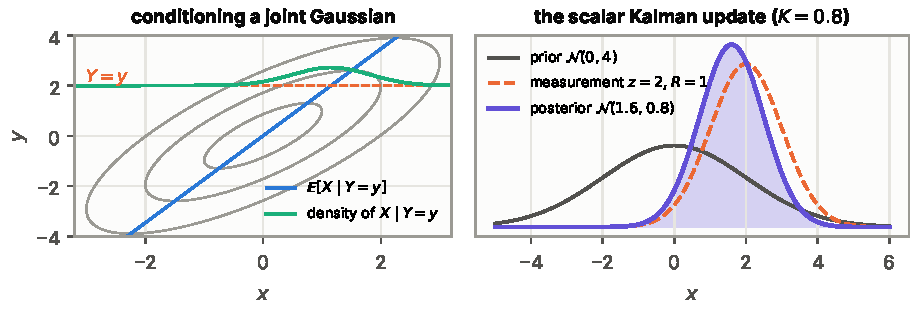
\includegraphics[width=\linewidth]{figures/ch03_gaussian.pdf}
\caption{Left: contours of a joint Gaussian of two scalars $(X,Y)$. Fixing $Y=y$
(dashed) slices it; the slice, divided by $p(y)$, is the Gaussian density
of $X\mid Y=y$, whose
mean lies on the regression line $\E[X\mid Y=y]$ and whose width does not
depend on $y$. Right: the Kalman update in one dimension, for a prediction
$\Normal(0,4)$ and a measurement $z=2$ with noise variance $R=1$
(\cref{ex:scalarkf}): the posterior is $\Normal(1.6,\,0.8)$, with the
gain $K=0.8$. The posterior lies between the prior and the measurement, closer
to the more precise one, and is narrower than both.}
\label{fig:gaussian}
\end{figure}

\section{The filter}

The Kalman filter applies to models in which the next state is a linear
function of the current state and of the control, and the measurement is a
linear function of the state, each with added Gaussian noise. The matrix
$F_t$ says how the state evolves by itself, $B_t$ how the control acts on
it, and $H_t$ which combination of the state the sensor sees.

\begin{definition}{Linear-Gaussian model}{lgmodel}
\begin{align*}
  \x_{t+1}&=F_t\x_t+B_t\uu_t+\w_t, & \w_t&\sim\Normal(\vect0,Q_t),\\
  \z_{t}&=H_t\x_t+\vv_t, & \vv_t&\sim\Normal(\vect0,R_t),
\end{align*}
with $\x_0\sim\Normal(\hx_0,P_0)$, $R_t\succ0$, and all noises
independent of each other and of $\x_0$.
\end{definition}

Two symbols are used throughout the book: a bar marks a \emph{predicted}
quantity (before the measurement), $\bx$ and $\bar P$; a hat marks an
\emph{updated} estimate (after it), $\hx$, with covariance $P$.

\paragraph{The update in one dimension.} The heart of the filter is
visible when the state is a single number $x$. Before the measurement,
the filter believes $x\sim\Normal(\bar x,\bar P)$. A sensor reads
$z=x+v$, with a noise $v\sim\Normal(0,R)$ independent of $x$. These are two
noisy pieces of information about the same number: the prediction
$\bar x$, of variance $\bar P$, and the reading $z$, of variance $R$. The pair $(x,z)$ is jointly Gaussian (\cref{lem:affine}), and, because
$x$ and $v$ are independent,
\[
  \Cov(x,z)=\Cov(x,x+v)=\Var(x)+\Cov(x,v)=\bar P+0,\qquad
  \Var(z)=\Var(x)+\Var(v)=\bar P+R .
\]
\Cref{thm:conditioning}, with $X=x$, $Y=z$, $\mu_x=\mu_y=\bar x$,
$\Sigma_{xy}=\bar P$ and $\Sigma_{yy}=\bar P+R$, gives the belief after the
measurement, $x\mid z\sim\Normal(\hat x,P)$, with the mean
$\bar x+\frac{\bar P}{\bar P+R}(z-\bar x)$ and the variance
$\bar P-\frac{\bar P^2}{\bar P+R}$. Naming the fraction $K$:
\begin{equation}\label{eq:scalarkf}
  \hat x=\bar x+K\,(z-\bar x),\qquad K=\frac{\bar P}{\bar P+R},\qquad
  P=(1-K)\,\bar P=\frac{\bar PR}{\bar P+R}.
\end{equation}
Three things can be read from these formulas.
\begin{itemize}[nosep]
  \item \emph{A weighted average.} $\hat x=(1-K)\,\bar x+K\,z$, with a
    weight $K$ between $0$ and $1$, the \emph{gain}. If the prediction is
    poor compared with the sensor ($\bar P\gg R$), $K$ is close to $1$ and
    the estimate follows the reading. If the sensor is poor, $K$ is close
    to $0$ and the reading is almost ignored.
  \item \emph{Precisions add.} The inverse of a variance is called a
    \emph{precision}, and
    $1/P=(\bar P+R)/(\bar PR)=1/R+1/\bar P$. The result is more precise
    than either source.
  \item \emph{The new variance does not depend on the reading.} $P$ is
    known before $z$ arrives.
\end{itemize}

\begin{example}{One update in one dimension}{scalarkf}
The prediction is $\Normal(0,4)$: the filter expects $x$ near $0$, give or
take $2$. The sensor has noise variance $R=1$ and reads $z=2$. Then $K=\bar P/(\bar P+R)=4/(4+1)=0.8$: the sensor is four times more
precise than the prediction, so the estimate moves four fifths of the way
towards the reading, $\hat x=\bar x+K(z-\bar x)=0+0.8\times(2-0)=1.6$. Its
variance is $P=(1-K)\bar P=(1-0.8)\times4=0.8$, smaller than both $4$ and
$1$; in precisions, $1/0.8=1.25=1/4+1/1$. This is the example drawn in \cref{fig:gaussian}, right.
\end{example}

The general filter is the same computation with matrices. It adds the
prediction step, and a matrix $H$ for sensors that measure a combination
of the coordinates of the state instead of the state itself.

\begin{theorem}{Kalman filter}{kf}
Under \cref{def:lgmodel}, every belief is Gaussian,
$\bel(\x_t)=\Normal(\hx_t,P_t)$, and $\belbar(\x_{t+1})=
\Normal(\bx_{t+1},\bar P_{t+1})$, with
\begin{align}
  &\textbf{predict:} & \bx_{t+1}&=F_t\hx_t+B_t\uu_t, &
  \bar P_{t+1}&=F_tP_tF_t\T+Q_t, \label{eq:kfpredict}\\
  &\textbf{update:} & \y&=\z_{t+1}-H\bx_{t+1}, & S&=H\bar P_{t+1}H\T+R,
  \notag\\
  && K&=\bar P_{t+1}H\T S^{-1}, & \hx_{t+1}&=\bx_{t+1}+K\y,\quad
  P_{t+1}=(I-KH)\bar P_{t+1}, \label{eq:kfupdate}
\end{align}
where $H$ and $R$ are taken at time $t+1$.
\end{theorem}

\begin{proof}
By induction on $t$. The belief $\bel(\x_0)=\Normal(\hx_0,P_0)$ is
Gaussian by assumption. Suppose that $\bel(\x_t)=\Normal(\hx_t,P_t)$.
Everything below is conditional on the past data (the controls and the
measurements up to time $t$); to lighten the notation, write $\x$, $\z$,
$\vv$, $\bx$ and $\bar P$ for $\x_{t+1}$, $\z_{t+1}$, $\vv_{t+1}$,
$\bx_{t+1}$ and $\bar P_{t+1}$.

\emph{Predict.} $\x_{t+1}=F_t\x_t+B_t\uu_t+\w_t$, where $\x_t\sim
\Normal(\hx_t,P_t)$, $B_t\uu_t$ is known, and $\w_t\sim\Normal(\vect0,
Q_t)$ is independent of $\x_t$ and of the past. \Cref{lem:affine}, with
$A=F_t$, $\vect b=B_t\uu_t$ and $W=\w_t$, gives
$\x_{t+1}\sim\Normal(F_t\hx_t+B_t\uu_t,\;F_tP_tF_t\T+Q_t)$: this is
\eqref{eq:kfpredict}.

\emph{The pair (state, measurement).} $\z=H\x+\vv$, with
$\vv\sim\Normal(\vect0,R)$ independent of $\x$. The pair $(\x,\z)$ is an
affine map of the independent Gaussians $\x$ and $\vv$, hence jointly
Gaussian (\cref{lem:affine}), with
\begin{align*}
  \bmu_y&=\E[H\x+\vv]=H\bx,\\
  \Sigma_{xy}&=\Cov(\x,H\x+\vv)=\Cov(\x,\x)H\T+\Cov(\x,\vv)
  =\bar PH\T+0,\\
  \Sigma_{yy}&=\Cov(H\x+\vv)=H\bar PH\T+R=S,
\end{align*}
the last line because the covariances of the independent $H\x$ and $\vv$
add.

\emph{Update.} \Cref{thm:conditioning}, with $X=\x$ and $Y=\z$, gives a
Gaussian with the mean and covariance
\begin{align*}
  \bx+\Sigma_{xy}\Sigma_{yy}^{-1}(\z-\bmu_y)
  &=\bx+\bar PH\T S^{-1}(\z-H\bx)=\bx+K\y,\\
  \bar P-\Sigma_{xy}\Sigma_{yy}^{-1}\Sigma_{yx}
  &=\bar P-\bar PH\T S^{-1}H\bar P=\bar P-KH\bar P=(I-KH)\bar P,
\end{align*}
using $\Sigma_{yx}=\Sigma_{xy}\T=H\bar P$ ($\bar P$ is symmetric). This
is \eqref{eq:kfupdate}, and $\bel(\x_{t+1})$ is Gaussian.
\end{proof}

The quantity $\y$ is the \emph{innovation}: what the measurement says that
the prediction did not. Its covariance is $S$ (Exercise~\ref{ex:innov}),
and $K$ is the \emph{Kalman gain}. In one dimension with $H=1$ these are
the formulas \eqref{eq:scalarkf}. The addition of precisions also holds in
any dimension.


\begin{proposition}{Information form}{information}
If $\bar P$ and $R$ are invertible, then
\[
  P^{-1}=\bar P^{-1}+H\T R^{-1}H\qquad\text{and}\qquad K=PH\T R^{-1}.
\]
\end{proposition}

\begin{proof}
To show that $P$ is the inverse of $\bar P^{-1}+H\T R^{-1}H$, multiply the
two and check that the product is $I$. Two identities are used:
$H\bar PH\T=S-R$, from the definition of $S$, and
\[
  S^{-1}(S-R)R^{-1}=S^{-1}SR^{-1}-S^{-1}RR^{-1}=R^{-1}-S^{-1} .
\]
Then, with $P=\bar P-\bar PH\T S^{-1}H\bar P$ from \cref{thm:kf}:
\begin{align*}
  P(\bar P^{-1}+H\T R^{-1}H)
  &=I+\bar PH\T R^{-1}H-\bar PH\T S^{-1}H
  &&\text{expand; }\bar P\bar P^{-1}=I\\
  &\qquad-\bar PH\T S^{-1}(H\bar PH\T)R^{-1}H\\
  &=I+\bar PH\T\bigl[R^{-1}-S^{-1}-S^{-1}(S-R)R^{-1}\bigr]H
  &&H\bar PH\T=S-R\\
  &=I+\bar PH\T\bigl[R^{-1}-S^{-1}-(R^{-1}-S^{-1})\bigr]H=I .
\end{align*}
For the gain:
\begin{align*}
  PH\T R^{-1}
  &=\bar PH\T R^{-1}-\bar PH\T S^{-1}(H\bar PH\T)R^{-1}
   =\bar PH\T R^{-1}-\bar PH\T S^{-1}(S-R)R^{-1}\\
  &=\bar PH\T R^{-1}-\bar PH\T(R^{-1}-S^{-1})=\bar PH\T S^{-1}=K .
\end{align*}
\end{proof}

\begin{inwords}
Information (inverse covariance) adds: what we knew, plus what the
measurement tells, and the measurement's contribution $H\T R^{-1}H$ does
not depend on what we knew. An update can only reduce the uncertainty, in every direction, as the
next paragraph shows. A direction $\vect n$ that the sensor
does not see ($H\vect n=\vect0$) receives no information from the
measurement itself: $\vect n\T P^{-1}\vect n=\vect n\T\bar P^{-1}\vect n$.
Its variance can still decrease, but only through its correlation with the
directions that the sensor does see; this is how a position fix can
correct a heading.
\end{inwords}

\emph{Why an update never increases a variance.} The variance of the
error along a direction $\vect n$ is $\vect n\T P\vect n$. With
$P=\bar P-\bar PH\T S^{-1}H\bar P$,
\[
  \vect n\T P\vect n=\vect n\T\bar P\vect n-\vect m\T S^{-1}\vect m,
  \qquad\vect m=H\bar P\vect n,
\]
because $\vect n\T\bar PH\T=(H\bar P\vect n)\T=\vect m\T$, $\bar P$ being
symmetric. $S^{-1}$ is positive definite (the inverse of the positive
definite $S$), so $\vect m\T S^{-1}\vect m\ge0$ and
$\vect n\T P\vect n\le\vect n\T\bar P\vect n$.

\begin{proposition}{Joseph form}{joseph}
Let the prediction error $\x-\bx$ have mean zero and covariance $\bar P$
and be independent of the measurement noise $\vv$. For \emph{any} gain
$K$, the error of the estimate $\hx=\bx+K(\z-H\bx)$ has covariance
\begin{equation}\label{eq:joseph}
  P_K=(I-KH)\bar P(I-KH)\T+KRK\T,
\end{equation}
which is positive semi-definite. For the Kalman gain it equals
$(I-KH)\bar P$.
\end{proposition}

\begin{proof}
\emph{The error.} With $\z=H\x+\vv$,
\[
  \x-\hx=\x-\bx-K(H\x+\vv-H\bx)=(I-KH)(\x-\bx)-K\vv ,
\]
a sum of two independent zero-mean terms, with the covariances
$(I-KH)\bar P(I-KH)\T$ and $K RK\T$ (by $\Cov(AX)=A\Cov(X)A\T$). The
covariances of independent terms add, which gives \eqref{eq:joseph}: a
sum of two positive semi-definite matrices, hence positive
semi-definite.

\emph{The Kalman gain.} Expand the product:
\begin{align*}
  P_K&=\bar P-KH\bar P-\bar PH\T K\T+KH\bar PH\T K\T+KRK\T\\
  &=\bar P-KH\bar P-\bar PH\T K\T+KSK\T
  &&H\bar PH\T+R=S .
\end{align*}
With $K=\bar PH\T S^{-1}$, the last term is $KSK\T=\bar PH\T S^{-1}SK\T=
\bar PH\T K\T$, which cancels the third, and $P_K=\bar P-KH\bar P=(I-KH)
\bar P$.
\end{proof}

The short form $(I-KH)\bar P$ is the difference of two positive
semi-definite matrices; rounding errors can make it slightly asymmetric
or indefinite, and the next update may then fail. The Joseph form is a sum
of positive semi-definite terms and does not have that problem, which is
why the code uses it. It also gives the true error covariance when the
gain is wrong, for instance because the filter was given the wrong $R$
(Exercise~\ref{ex:wrongR}).

\section{A linear robot}
\label{sec:linmower}

The pose model of Chapter~\ref{ch:statespace} is not linear: the heading
enters through $\cos$ and $\sin$. We make it linear honestly, with the
compass. The robot drives from $\p_t$ to $\p_{t+1}$ along the heading
$\theta_{t+1}$ that it has after its turn. Let
$c_{t+1}=\wrap(\theta_{t+1}+\nu_{t+1})$ be the compass reading of that
heading (\cref{sec:sensors}). With the heading read off the compass, the
displacement is a \emph{known input}. The turn error $\varepsilon_\delta$
no longer matters: whatever heading the robot ends up with, the compass
reads it. The position obeys
\begin{equation}\label{eq:linmower}
  \p_{t+1}=\p_t+s_t\begin{pmatrix}\cos c_{t+1}\\\sin c_{t+1}\end{pmatrix}
  +\w_t,\qquad\z_{t+1}=\p_{t+1}+\vv_{t+1},
\end{equation}
so $F=B=H=I$ and $R=\sigma_{\mathrm{gps}}^2I=64\,I$
($\sigma_{\mathrm{gps}}=8$). The noise $\w_t$ is the difference between
the true displacement and the one computed from the compass. The true
displacement is $(s_t+\varepsilon_s)(\cos\theta_{t+1},\sin\theta_{t+1})$
with $\theta_{t+1}=c_{t+1}-\nu_{t+1}$. To first order in the small angle
$\nu=\nu_{t+1}$, writing $c=c_{t+1}$,
\[
  \cos(c-\nu)\approx\cos c+\nu\sin c,\qquad
  \sin(c-\nu)\approx\sin c-\nu\cos c ,
\]
and, dropping the product $\varepsilon_s\nu$ of two small noises,
\[
  (s_t+\varepsilon_s)\begin{pmatrix}\cos(c-\nu)\\\sin(c-\nu)\end{pmatrix}
  \approx s_t\begin{pmatrix}\cos c\\\sin c\end{pmatrix}
  +\varepsilon_s\begin{pmatrix}\cos c\\\sin c\end{pmatrix}
  +(-\nu)\,s_t\begin{pmatrix}-\sin c\\\cos c\end{pmatrix}.
\]
The first term is the computed displacement, and the other two are the
noise:
\[
  \w_t\approx G_t\begin{pmatrix}\varepsilon_s\\-\nu_{t+1}\end{pmatrix},\quad
  G_t=\begin{pmatrix}\cos c_{t+1}&-s_t\sin c_{t+1}\\
  \sin c_{t+1}&s_t\cos c_{t+1}\end{pmatrix},\qquad
  Q_t=G_t\diag(\sigma_s^2,\sigma_c^2)\,G_t\T ,
\]
the covariance following from $\Cov(AX)=A\Cov(X)A\T$, with
$\Cov(\varepsilon_s,-\nu_{t+1})=\diag(\sigma_s^2,\sigma_c^2)$ for
independent noises.
This is the computation of \cref{sec:errors} again: an error on the
distance moves the robot along its heading, and an error on the heading,
here the compass error, moves it sideways by $s_t$ per radian. $G_t$ is the upper $2\times2$ block of the matrix
$V=\bigl(\begin{smallmatrix}\cos\theta'&-s\sin\theta'\\\sin\theta'&s\cos\theta'\\0&1\end{smallmatrix}\bigr)$
of \eqref{eq:firstorder}, whose columns give the effects on the pose of a
distance error and of a heading error, with the heading $\theta'$ replaced
by the compass reading $c_{t+1}$.
One more approximation is made, beyond the first order: the compass noise
$\nu_{t+1}$ enters both the known input $c_{t+1}$ and the noise $\w_t$, so
$\w_t$ is not exactly independent of the input. The effect is small
($\sigma_c=0.02$\,rad), and the consistency test of \cref{fig:kfnees}
shows that the filter is not misled by it.
$Q_t$ is long along the heading (step noise) and thin across it (compass
noise), and it turns with the robot. A time-varying $Q_t$ is no problem:
nothing in \cref{thm:kf} needs it to be constant.

\Cref{fig:kftrack} shows the filter on the standard run. Once it has
settled (after the first 20 steps), its RMS position error is $1.99$,
against $11.3$ for the raw GPS fixes (notebook~02): filtering divides the
error by $11.3/1.99\approx5.7$.

\begin{figure}[ht]
\centering
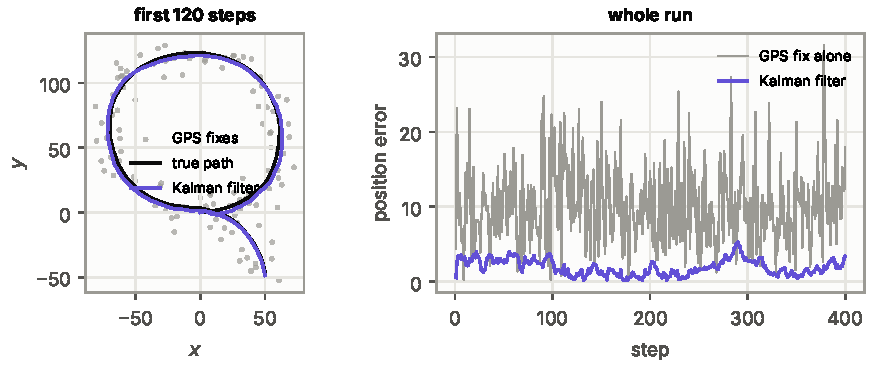
\includegraphics[width=\linewidth]{figures/ch03_kf_track.pdf}
\caption{The Kalman filter of the linear robot, which takes its heading
from the compass and corrects its position with GPS fixes
($\sigma_{\mathrm{gps}}=8$), on the standard run (seed 1). Left: the true
path, the GPS fixes and the filter's estimate over the first 120 steps.
Right: the position error of each GPS fix and of the filter over the
whole run.}
\label{fig:kftrack}
\end{figure}

\section{The gain settles}

When $F$, $H$, $Q$ and $R$ are fixed in advance, $P_t$ and $K_t$ do not
depend on the measurements: only on these matrices and on $P_0$. (In the
compass--GPS filter they depend on the compass readings, through $Q_t$,
but not on the GPS fixes.) For a time-invariant model the predicted covariance obeys the
\emph{Riccati recursion} $\bar P\mapsto F\bigl(\bar P-\bar PH\T(H\bar PH\T
+R)^{-1}H\bar P\bigr)F\T+Q$, which converges, under mild conditions, to a
unique fixed point. (The conditions are called detectability and
stabilisability. Roughly: the sensor sees every direction of the state in
which the error would otherwise grow, and the noise $Q$ excites every such
direction. The general result is not proved here; see Bar-Shalom, Li and
Kirubarajan in the references.) The scalar case can be solved by hand, and
\cref{fig:riccati} shows the convergence.

\begin{proposition}{Steady state of a random walk observed in noise}{steady}
For the scalar model $x_{t+1}=x_t+w_t$, $z_t=x_t+v_t$ with variances $q>0$
and $r>0$, the steady-state predicted and updated variances are
\[
  \bar P_\infty=\frac{q+\sqrt{q^2+4qr}}2,\qquad
  P_\infty=\frac{\bar P_\infty r}{\bar P_\infty+r}=\bar P_\infty-q .
\]
\end{proposition}

\begin{proof}
\emph{The fixed point.} With $F=H=1$, the update gives
$P=\bar Pr/(\bar P+r)$ (\cref{eq:scalarkf}) and the next prediction gives
$\bar P=P+q$. At a fixed point both hold with the same $\bar P$:
\begin{align*}
  \bar P&=\frac{\bar Pr}{\bar P+r}+q\\
  \bar P(\bar P+r)&=\bar Pr+q(\bar P+r)
  &&\text{multiply by }\bar P+r\\
  \bar P^2-q\bar P-qr&=0
  &&\text{expand; }\bar Pr\text{ cancels.}
\end{align*}
This quadratic has the roots $\bigl(q\pm\sqrt{q^2+4qr}\bigr)/2$; one is
negative, and the positive one is $\bar P_\infty$. Then
$P_\infty=\bar P_\infty-q$ from $\bar P=P+q$.

\emph{Convergence.} One cycle maps $\bar P$ to
$g(\bar P)=\bar Pr/(\bar P+r)+q$, whose derivative is
\[
  g'(\bar P)=\frac{r(\bar P+r)-\bar Pr}{(\bar P+r)^2}
  =\frac{r^2}{(\bar P+r)^2}.
\]
After the first cycle $\bar P\ge q$, since $g(\bar P)\ge q$. On
$[q,\infty)$, $0<g'\le c$ with $c=r^2/(q+r)^2<1$. By the mean value
theorem, $\abs{g(a)-g(b)}=g'(\xi)\abs{a-b}\le c\,\abs{a-b}$ for $a,b$ in
that interval. With $b=\bar P_\infty$, a fixed point, the distance to
$\bar P_\infty$ is multiplied by at most $c$ at each cycle, so after $t$
more cycles it is at most $c^t$ times the initial distance, which tends to
$0$: the recursion converges to $\bar P_\infty$ from any start.
\end{proof}

\begin{figure}[ht]
\centering
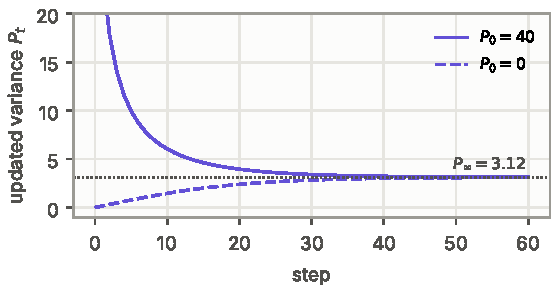
\includegraphics{figures/ch03_riccati.pdf}
\caption{The updated variance $P_t$ of the scalar model
$x_{t+1}=x_t+w_t$, $z_t=x_t+v_t$, with $q=0.16$ and $r=64$ (the values of
the robot along its heading), from an uncertain start $P_0=40$ (solid) and
from an exactly known start $P_0=0$ (dashed). Both converge to the same $P_\infty$: the filter forgets
its initial uncertainty.}
\label{fig:riccati}
\end{figure}

For the robot, $r=\sigma_{\mathrm{gps}}^2=64$ in both directions. Along
the heading, $q=\sigma_s^2=0.4^2=0.16$, and
\[
  \bar P_\infty=\frac{0.16+\sqrt{0.16^2+4\times0.16\times64}}{2}
  =\frac{0.16+6.402}{2}=3.28,\qquad P_\infty=3.28-0.16=3.12 .
\]
Across it, $q=(s\sigma_c)^2=(4\times0.02)^2=0.0064$, and the same formulas
give $\bar P_\infty=(0.0064+1.280)/2=0.643$ and $P_\infty=0.64$. If the heading
were constant, the RMS error would therefore settle at
$\sqrt{3.12+0.64}=1.94$. Because the heading turns, the long axis of $Q_t$
rotates and the two directions mix. Averaged over the headings, $Q_t$ is
about $\tfrac12(0.16+0.0064)\,I=0.0832\,I$: with $q_1=0.16$ along the
heading $c$ and $q_2=0.0064$ across it, the entries of $Q_t$ are
$q_1\cos^2c+q_2\sin^2c$, $q_1\sin^2c+q_2\cos^2c$ on the diagonal and
$(q_1-q_2)\sin c\cos c$ off it, and over a full turn $\cos^2$ and
$\sin^2$ average to $\tfrac12$ and $\sin c\cos c$ to $0$. Then \cref{prop:steady} with $q=0.0832$ gives
$\bar P_\infty=(0.0832+\sqrt{0.0832^2+4\times0.0832\times64})/2=2.35$ and
$P_\infty=2.35-0.08=2.27$ per axis, a trace of $2\times2.27=4.5$. The filter's
own covariance indeed settles around $\operatorname{tr}P\approx4.5$, i.e.\
an RMS of $2.1$, and the measured RMS error over 20 runs (seeds 0 to 19,
started at the true pose with $P_0=\diag(400,400)$, the first 20 steps
left out) is $2.11$ (notebook~02). The filter's covariance is
telling the truth, which is the subject of the next section.

\section{Is the filter honest? NEES}

A small error is not enough: the filter must also \emph{know} how large
its error is, because its covariance is what the next update, and every
decision downstream, relies on.

\begin{definition}{NEES}{nees}
The \emph{normalised estimation error squared} at time $t$ is
\[
  \NEES_t=(\x_t-\hx_t)\T P_t^{-1}(\x_t-\hx_t).
\]
\end{definition}

The NEES is the squared error measured in units of the covariance the
filter claims: in one dimension it is $(x-\hat x)^2/P$, which is $1$ on
average when the claim is right. An error of $3$ with a claimed standard
deviation of $1$ gives a NEES of $9$: a ``three-sigma'' error, which
should be rare. Recall that $\chi^2_n$ (chi-squared with
$n$ degrees of freedom) is the distribution of the sum of the squares of
$n$ independent standard normal variables; its mean is $n$.

For the Kalman filter of a linear-Gaussian model, the hypothesis of the
next proposition is the conclusion of \cref{thm:kf}: given the data, the
error $\x_t-\hx_t$ is $\Normal(\vect0,P_t)$.

\begin{proposition}{NEES of a consistent filter}{neeschi2}
If $\x_t-\hx_t\sim\Normal(\vect0,P_t)$ with $P_t\succ0$ in $\R^n$, then
$\NEES_t\sim\chi^2_n$, so $\E[\NEES_t]=n$. If $\NEES^{(1)},\dots,
\NEES^{(N)}$ are the values from $N$ independent runs, then
$N\cdot\frac1N\sum_k\NEES^{(k)}\sim\chi^2_{nN}$.
\end{proposition}

\begin{proof}
Let $L$ with $LL\T=P_t$ (Cholesky), and $\vect g=L^{-1}(\x_t-\hx_t)$. By
\cref{lem:affine}, $\vect g$ is Gaussian with mean $\vect0$ and
covariance $L^{-1}P_tL^{-\mathsf T}=L^{-1}LL\T L^{-\mathsf T}=I$, so its
coordinates are independent standard normals (\cref{lem:uncorr}). Then
\[
  \NEES_t=(\x_t-\hx_t)\T(LL\T)^{-1}(\x_t-\hx_t)
  =\bigl(L^{-1}(\x_t-\hx_t)\bigr)\T L^{-1}(\x_t-\hx_t)
  =\vect g\T\vect g=\sum_{i=1}^ng_i^2 ,
\]
a sum of $n$ squared independent standard normals: $\chi^2_n$, of mean
$n$, since each square has the mean $\E[g_i^2]=\Var(g_i)=1$. The $N$ runs are independent, so the sum
of their NEES is a sum of $nN$ squares of independent standard normals,
that is $\chi^2_{nN}$.
\end{proof}

A two-sided $95\%$ acceptance band for the average NEES over $N$ runs is
therefore
\[
  \bigl[\chi^2_{nN}(0.025),\;\chi^2_{nN}(0.975)\bigr]\big/N,
\]
where $\chi^2_k(p)$ is the $p$-quantile of $\chi^2_k$: the value below
which $\chi^2_k$ falls with probability $p$. For example, with $n=2$
and $N=50$ runs, $\chi^2_{100}(0.025)=74.2$ and
$\chi^2_{100}(0.975)=129.6$, and the band is $[1.48,\,2.59]$
(notebook~02). Above it, the
filter is \emph{over-confident}: it claims more precision than it has.
Below it, it is \emph{pessimistic}. For the test to be fair, the initial
estimate must itself be drawn from the initial belief,
$\hx_0\sim\Normal(\x_0,P_0)$; starting exactly at the truth with a large
$P_0$ would make the first steps look pessimistic.

\begin{figure}[ht]
\centering
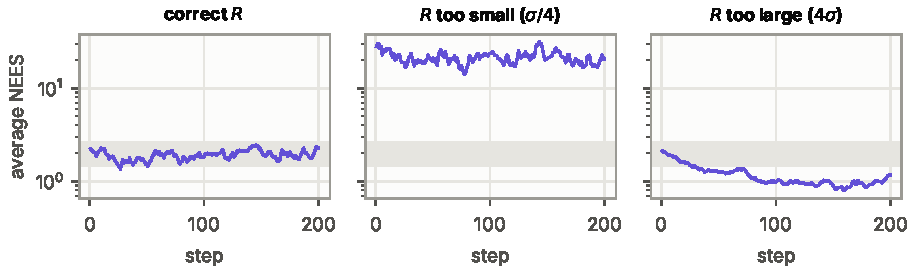
\includegraphics[width=\linewidth]{figures/ch03_kf_nees.pdf}
\caption{Average NEES over 50 runs (log scale) for the Kalman filter of
the linear robot (compass heading, GPS fixes with
$\sigma_{\mathrm{gps}}=8$); grey: the $95\%$ band for $n=2$,
$[1.48,\,2.59]$. Left: the correct $R$,
inside the band. Middle: the filter believes that the standard deviation
of the GPS is 4 times smaller than it is ($R/16$): over-confident by an
order of magnitude. Right: it believes it is 4 times larger ($16R$):
pessimistic.}
\label{fig:kfnees}
\end{figure}

\begin{inwords}
NEES asks: ``are the errors as big as the filter says they are?'' A
filter that believes its sensor too much is jumpy \emph{and} certain; one
that believes it too little is sluggish and doubtful. NEES needs the
truth, so it is a simulation tool. On real data the same idea is applied
to the innovations: for a correct filter the innovation is
$\Normal(\vect0,S)$ (Exercise~\ref{ex:innov}), so
$\y\T S^{-1}\y\sim\chi^2_{\dim\z}$ by the same argument (the \emph{NIS}
test), and that one only needs the data.
\end{inwords}

\begin{practice}[\nb{02\_kalman\_filter.ipynb}, \code{kf.py}, \code{metrics.py}]
\code{KalmanFilter} is the generic filter of \cref{thm:kf}, with the
Joseph update; \code{CompassGpsKF} builds $Q_t$ from the compass reading
at each step. \code{nees} and \code{nees\_bounds} implement
\cref{def:nees} and the $\chi^2$ band. The notebook checks the scalar
example $\Normal(0,4)$ updated by a measurement $2$ of variance $1$
(posterior $\Normal(8/5,4/5)$, gain $0.8$), shows the gain settling, and
reproduces \cref{fig:kfnees}.
\end{practice}

\begin{mower}
Wheel odometry plus RTK-GNSS is exactly this filter, and a common design
for robot mowers. RTK fixes are accurate to about 2\,cm with an open sky,
but degrade near trees and walls, sometimes without warning. A filter
with a fixed, optimistic $R$ is then the middle panel of
\cref{fig:kfnees}: it follows a bad fix with full confidence. Monitoring
the NIS and inflating $R$ (or rejecting the fix) when it leaves its band
is a cheap and effective guard.
\end{mower}

\section*{What to remember from this chapter}
\addcontentsline{toc}{section}{What to remember}

\begin{enumerate}[nosep]
  \item For a linear model with Gaussian noises, the belief is exactly
    Gaussian, and the Bayes filter reduces to formulas on its mean and
    covariance: the Kalman filter (\cref{thm:kf}).
  \item Predict: the mean follows the model and the covariance grows,
    $\bar P=FPF\T+Q$. Update: the mean moves by gain times innovation,
    $\hx=\bx+K\y$, and the covariance shrinks.
  \item The gain weighs the prediction against the measurement according
    to their precisions. In information form, precisions add:
    $P^{-1}=\bar P^{-1}+H\T R^{-1}H$.
  \item The covariance and the gain do not depend on the measurements, and
    for a time-invariant model they settle to constants.
  \item A filter is \emph{consistent} when its errors are as large as its
    covariance says. The NEES test checks this in simulation, the NIS test
    on real data. A wrong $R$ or $Q$ makes the filter over-confident or
    pessimistic.
\end{enumerate}

\FloatBarrier
\section*{Exercises}
\addcontentsline{toc}{section}{Exercises}

\begin{enumerate}[label=\textbf{3.\arabic*},ref=3.\arabic*]
\item\label{ex:innov} Show that, for the Kalman filter, the innovation
  $\y=\z-H\bx$ has mean zero and covariance $S$, and that it is
  uncorrelated with the error of the estimate \emph{after} the update,
  i.e.\ $\Cov(\x-\hx,\y)=0$.
\item\label{ex:fusion} Two independent sensors measure the same scalar,
  with variances $r_1$ and $r_2$, and there is no prior ($\bar P=\infty$).
  Using \cref{prop:information} (precisions add,
$P^{-1}=\bar P^{-1}+H\T R^{-1}H$, and $K=PH\T R^{-1}$), show that the
optimal estimate is the
  inverse-variance weighted average and give its variance. What happens
  when $r_2\to\infty$?
\item\label{ex:steadynum} Use \cref{prop:steady} to compute the
  steady-state gain $K_\infty=\bar P_\infty/(\bar P_\infty+r)$ along the
  heading for the robot ($q=0.16$, $r=64$). How many past GPS fixes does
  the filter effectively average?
\item\label{ex:wrongR} A Kalman filter is run with a wrong measurement
  covariance $R'$ while the true one is $R$. Show that the covariance it
  reports follows the Riccati recursion with $R'$, while the covariance of
  its actual error follows a linear recursion that uses the filter's gain
  and the true $R$; write that recursion. Explain the middle panel of
  \cref{fig:kfnees}.
\end{enumerate}

\subsection*{Solutions}

\solution{3.1} Everything is conditional on the past data, and the
prediction error $\x-\bx$ has mean $\vect0$ and covariance $\bar P$
(\cref{thm:kf}).

\emph{Mean and covariance of the innovation.} With $\z=H\x+\vv$,
\[
  \y=\z-H\bx=H(\x-\bx)+\vv .
\]
Both terms have mean zero, so $\E[\y]=\vect0$. They are independent (the
noise $\vv$ is independent of the state and of the past), so their
covariances add:
$\Cov(\y)=H\,\Cov(\x-\bx)\,H\T+\Cov(\vv)=H\bar PH\T+R=S$.

\emph{The updated error and the innovation.} After the update,
$\x-\hx=\x-\bx-K\y$. The cross-covariance is linear in each argument, so
\[
  \Cov(\x-\hx,\y)=\Cov(\x-\bx,\y)-K\Cov(\y,\y)=\Cov(\x-\bx,\y)-KS .
\]
The first term is
$\Cov(\x-\bx,\,H(\x-\bx)+\vv)=\Cov(\x-\bx,\x-\bx)H\T+\Cov(\x-\bx,\vv)
=\bar PH\T+0$, and for the Kalman gain $KS=\bar PH\T S^{-1}S=\bar PH\T$.
So
\[
  \Cov(\x-\hx,\y)=\bar PH\T-\bar PH\T=0 .
\]
The updated error is uncorrelated with the innovation, and, the two being
jointly Gaussian, independent of it (\cref{lem:uncorr}): the filter has
extracted everything the measurement had to say.

\solution{3.2} \emph{The estimate in information form.} By
\cref{prop:information}, $P^{-1}=\bar P^{-1}+H\T R^{-1}H$ and
$K=PH\T R^{-1}$. The update can be written
$\hx=\bx+K(\z-H\bx)=(I-KH)\bx+K\z$, and
\[
  I-KH=I-PH\T R^{-1}H=P\bigl(P^{-1}-H\T R^{-1}H\bigr)=P\bar P^{-1},
\]
so
\[
  \hx=P\bigl(\bar P^{-1}\bx+H\T R^{-1}\z\bigr),\qquad
  P^{-1}=\bar P^{-1}+H\T R^{-1}H .
\]

\emph{No prior.} ``No prior'' is the limit $\bar P\to\infty$, where the
prior precision $\bar P^{-1}$ tends to $0$. Then
$P^{-1}=H\T R^{-1}H$ and $\hx=PH\T R^{-1}\z$.

\emph{Two sensors.} Stack the two readings into $\z=(z_1,z_2)$: both
measure the same scalar $x$, so $H=(1,1)\T$, and the noises are
independent, so $R=\diag(r_1,r_2)$. Then
\[
  H\T R^{-1}H=\frac1{r_1}+\frac1{r_2},\qquad
  H\T R^{-1}\z=\frac{z_1}{r_1}+\frac{z_2}{r_2},
\]
and
\[
  \hat x=\frac{z_1/r_1+z_2/r_2}{1/r_1+1/r_2}
  =\frac{r_2z_1+r_1z_2}{r_1+r_2},\qquad
  P=\frac{1}{1/r_1+1/r_2}=\frac{r_1r_2}{r_1+r_2}.
\]
This is the average of the readings weighted by their precisions $1/r_1$
and $1/r_2$, and its variance is smaller than both $r_1$ and $r_2$.

\emph{A useless second sensor.} When $r_2\to\infty$, the weight
$1/r_2$ tends to $0$: $\hat x\to z_1$ and $P\to r_1$. A sensor that tells
nothing is ignored; it never makes the estimate worse.

\solution{3.3} The robot along its heading is the model of
\cref{prop:steady} with $q=\sigma_s^2=0.16$ and $r=\sigma_{\mathrm{gps}}^2
=64$. The steady state is
\begin{align*}
  \bar P_\infty&=\frac{q+\sqrt{q^2+4qr}}{2}
  =\frac{0.16+\sqrt{0.0256+40.96}}{2}=3.28,\\
  K_\infty&=\frac{\bar P_\infty}{\bar P_\infty+r}=\frac{3.28}{3.28+64}
  =0.049 .
\end{align*}

\emph{An exponential moving average.} In steady state the update is
$\hat x_t=\bar x_t+K(z_t-\bar x_t)=(1-K)\bar x_t+Kz_t$, and the prediction
$\bar x_t=\hat x_{t-1}+d_{t-1}$ adds the known displacement. Leaving the
displacements aside, unrolling the recursion gives
\[
  \hat x_t=Kz_t+K(1-K)z_{t-1}+K(1-K)^2z_{t-2}+\cdots :
\]
the fix of $k$ steps ago has the weight $K(1-K)^k$, and the weights add up
to $K\sum_k(1-K)^k=K/K=1$. This is an \emph{exponential moving average},
a causal one: only past fixes enter.

\emph{How many fixes.} The weights decay by the factor $1-K$ per step;
their effective number is about $1/K=1/0.049\approx20$. The variance gives
the same count: an average of $m$ independent fixes has the variance
$r/m=64/m$, which equals $P_\infty=\bar P_\infty-q=3.12$ for
$m=64/3.12\approx20.5$.

\solution{3.4} \emph{What the filter reports.} The filter computes its
covariances and gains from its own recursion, as if the measurement
covariance were $R'$:
\[
  \bar P'\mapsto F\bigl(\bar P'-\bar P'H\T(H\bar P'H\T+R')^{-1}H\bar
  P'\bigr)F\T+Q,\qquad K'=\bar P'H\T(H\bar P'H\T+R')^{-1}.
\]
This is the Riccati recursion with $R'$, and $\bar P'$ is what it
reports.

\emph{What its error really is.} Its actual error obeys
$\x-\hx=(I-K'H)(\x-\bx)-K'\vv$, with the true noise
$\vv\sim\Normal(\vect0,R)$. \Cref{prop:joseph} holds for any gain, so the
actual covariance follows the linear recursion
\[
  P^{\mathrm{true}}=(I-K'H)\,\bar P^{\mathrm{true}}(I-K'H)\T+K'R{K'}\T,
  \qquad\bar P^{\mathrm{true}}\leftarrow FP^{\mathrm{true}}F\T+Q ,
\]
with the filter's gain $K'$ and the true $R$.

\emph{The middle panel of \cref{fig:kfnees}.} The filter believes
$R'=R/16$. Take the scalar values of \cref{prop:steady}: $F=H=1$,
$q=0.16$, the true $r=64$ and the believed $r'=64/16=4$. The filter's own
steady state is
\[
  \bar P'_\infty=\frac{0.16+\sqrt{0.16^2+4\times0.16\times4}}{2}=0.88,
  \qquad K'=\frac{0.88}{0.88+4}=0.181,
\]
against $0.049$ with the right $r$: the filter averages fewer fixes. The
variance it reports is $P'_\infty=\bar P'_\infty-q=0.88-0.16=0.72$. The
actual variance $P$ is the fixed point of the recursion above:
\begin{align*}
  P&=(1-K')^2(P+q)+K'^2r
  &&\text{fixed point}\\
  P\bigl(1-(1-K')^2\bigr)&=(1-K')^2q+K'^2r
  &&\text{collect }P\\
  P&=\frac{0.819^2\times0.16+0.181^2\times64}{1-0.819^2}
  =\frac{0.107+2.10}{0.329}\approx6.7
  &&K'=0.181,
\end{align*}
about nine times the reported $0.72$. NEES measures the actual error in
units of the reported covariance, hence values an order of magnitude
above the band.

\chapter{The extended Kalman filter}
\label{ch:ekf}

We now drop the compass. The state is the full pose $(p^x,p^y,\theta)$,
and both the motion model $f$ and the range--bearing model $h$ are
non-linear, so a Gaussian belief does not stay Gaussian. The \emph{extended}
Kalman filter keeps it Gaussian anyway: it replaces $f$ and $h$ by their
first-order Taylor expansions around the current estimate and then applies
the Kalman equations. This chapter derives the Jacobians, states the
filter, shows exactly what the linearisation throws away, and connects
the EKF update to Gauss--Newton optimisation.

\section{Linearisation}

The Kalman filter needs linear models. Near a given point every smooth
function looks linear: for a small deviation $\vect e$,
\[
  g(\vect a+\vect e)\approx g(\vect a)+G\,\vect e,\qquad
  G=\frac{\partial g}{\partial\x}(\vect a),\quad
  G_{ij}=\frac{\partial g_i}{\partial x_j}.
\]
The matrix $G$ is the \emph{Jacobian} of $g$ at $\vect a$: its column $j$
says how the output moves when the $j$-th input changes a little. In one
dimension it is the slope of the tangent (\cref{fig:linearisation}, left).
The EKF needs three Jacobians: $F$ and $V$ say how an error on the current
pose and an error on the control change the next pose, and $H$ says how an
error on the pose changes the measurement.

\begin{proposition}{Jacobians of the mower's models}{jacobians}
With $\theta'=\theta+\delta$, the motion model \eqref{eq:f} has
\[
  F=\frac{\partial f}{\partial\x}=\begin{pmatrix}1&0&-s\sin\theta'\\
  0&1&s\cos\theta'\\0&0&1\end{pmatrix},\qquad
  V=\frac{\partial f}{\partial\uu}=\begin{pmatrix}\cos\theta'&
  -s\sin\theta'\\\sin\theta'&s\cos\theta'\\0&1\end{pmatrix}.
\]
For a landmark at $\bell$, with $\vect{d}=\bell-\p$ and
$q=\norm{\vect{d}}^2$, the range--bearing model \eqref{eq:h} has
\[
  H=\frac{\partial h}{\partial\x}=\begin{pmatrix}-d_x/\sqrt q&-d_y/\sqrt q
  &0\\ d_y/q&-d_x/q&-1\end{pmatrix}.
\]
\end{proposition}

\begin{proof}
For $f$, differentiate component-wise; $\theta$ and $\delta$ enter only
through $\theta'$, whose derivative with respect to either is $1$. For the
range, $\nabla_{\p}\norm{\bell-\p}=-\vect{d}/\norm{\vect{d}}$. For the
bearing, $\partial\operatorname{atan2}(y,x)/\partial(x,y)=(-y,x)/
(x^2+y^2)$ and $\vect{d}$ depends on $\p$ with derivative $-I$, which
gives $(d_y,-d_x)/q$; the heading enters with coefficient $-1$. $\wrap$ is
locally a translation by a multiple of $2\pi$ and does not change
derivatives.
\end{proof}

Each entry can be read geometrically. The matrix $V$ is that of
\eqref{eq:firstorder}. The first two columns of $F$ say that a position
error is carried over unchanged. Its third column is the second column of
$V$: an error on the current heading acts exactly like a turn error, it
changes the new heading by the same amount and moves the mower sideways by
$s$ per radian (\cref{fig:tangent}). In $H$, the first row says that moving
towards the landmark shortens the range by the same amount, and that the
range does not depend on the heading. The second row says that moving
across the line of sight changes the bearing by the displacement divided
by the distance ($1/\sqrt q$ per unit), and that turning by an angle
changes the bearing by the opposite angle.

Hand-derived Jacobians are a classic source of bugs. The notebook and the
tests compare them with central finite differences; the largest
discrepancy is about $2\times10^{-9}$.

\section{The filter}

Suppose the belief is $\Normal(\hx,P)$, and write the true pose as
$\x_t=\hx+\vect e$ with $\vect e\sim\Normal(\vect0,P)$. Linearising $f$
around $(\hx,\uu)$ in both arguments,
\[
  \x_{t+1}=f(\hx+\vect e,\uu+\bepsilon)\approx f(\hx,\uu)+F\vect e
  +V\bepsilon .
\]
The right-hand side is an affine function of the independent Gaussians
$\vect e$ and $\bepsilon$, so by \cref{lem:affine} it is Gaussian with mean
$f(\hx,\uu)$ and covariance $FPF\T+VMV\T$: this is the prediction. In the
same way, around the predicted mean $\bx$,
\[
  \z=h(\x)+\vv\approx h(\bx)+H(\x-\bx)+\vv,
\]
a linear measurement of $\x$, up to the known constant $h(\bx)-H\bx$. The
Kalman update of \cref{thm:kf} then applies, with the innovation
$\z-h(\bx)$.

\begin{definition}{Extended Kalman filter}{ekf}
\begin{align*}
  &\textbf{predict:}&\bx&=f(\hx,\uu), & \bar P&=FPF\T+VMV\T,\\
  &\textbf{update:}& \y&=\z-h(\bx)\ \ (\text{bearings wrapped}), &
  S&=H\bar PH\T+R,\\
  && K&=\bar PH\T S^{-1}, & \hx&=\bx+K\y\ \ (\theta\ \text{wrapped}),
\end{align*}
$P=(I-KH)\bar P(I-KH)\T+KRK\T$, with $F,V$ evaluated at $(\hx,\uu)$ and
$H$ at $\bx$. With several visible landmarks, the measurements and the
rows of $H$ are stacked, and $R$ is block diagonal, with one copy of $R_1$
per landmark ($R=I\otimes R_1$).
\end{definition}

The \emph{mean} goes through the true non-linear functions; only the
\emph{covariance} goes through their Jacobians. The process noise enters
through the control, so its state-space covariance is $VMV\T$, of rank
two (\cref{prop:firstorder}); $\bar P$ stays positive definite because
$FPF\T$ is ($F$ is invertible, its determinant being $1$).

\begin{inwords}
The EKF pretends that, over the region where the mower probably is, the
world is flat: $f$ and $h$ are well approximated by their tangent planes.
It then applies the exact Kalman update to that flat world. When the
uncertainty is small compared with the curvature of $f$ and $h$, this is
an excellent approximation; when it is not, the next section shows what
goes wrong.
\end{inwords}

\paragraph{Angles.} Forgetting to wrap the bearing innovation is the most
common EKF bug in localisation. If the predicted bearing is $3.10$ and the
measured one is $-3.12$, the raw innovation is $-6.22$ instead of $+0.063$
(\cref{lem:wrap}), and the update throws the mower across the lawn.

On the standard run with four landmarks always in view, the EKF's position
RMSE is $1.13$, well below the range noise $\sigma_r=5$ and the
$\approx5$ units of position uncertainty that a bearing error of
$0.05$\,rad produces at 100 units. Each error component stays inside its
own $\pm2\sigma$ band about $95\%$ of the time: the filter is accurate and
honest.

\section{What linearisation throws away}

The EKF takes the mean of $g(X)$ to be $g$ of the mean. This is exact for
a linear $g$ and wrong for a curved one: where $g$ bends downwards, the
values of $g$ on both sides of the mean are below the tangent, and the
average of $g(X)$ is below $g(\bmu)$. The next proposition measures the
gap. In it, $\nabla^2g_i$ is the \emph{Hessian} of $g_i$, the matrix of its
second derivatives, and $\tr$ is the trace, the sum of the diagonal
entries.

\begin{proposition}{Second-order mean of a non-linear map}{secondorder}
Let $X\sim\Normal(\bmu,\Sigma)$ and let $g$ be four times continuously
differentiable with bounded fourth derivatives. Then
\[
  \E[g_i(X)]=g_i(\bmu)+\tfrac12\tr\bigl(\nabla^2g_i(\bmu)\,\Sigma\bigr)
  +O(\norm{\Sigma}^{2}),
\]
for each component $g_i$. The linearised mean $g(\bmu)$ is therefore
biased by $\tfrac12\tr(\nabla^2g_i\Sigma)$, to first order in $\Sigma$.
\end{proposition}

\begin{proof}
Taylor's theorem around $\bmu$ with $\vect{e}=X-\bmu$:
$g_i(X)=g_i(\bmu)+\nabla g_i\T\vect{e}+\tfrac12\vect{e}\T\nabla^2g_i
\vect{e}+\tfrac16D^3g_i[\vect{e},\vect{e},\vect{e}]+\rho(\vect{e})$ with
$|\rho(\vect{e})|\le C\norm{\vect{e}}^4$. Take expectations:
$\E[\vect{e}]=\vect0$,
$\E[\vect{e}\T A\vect{e}]=\E[\tr(A\vect e\vect e\T)]=\tr(A\Sigma)$, the
cubic term has expectation zero because the odd moments of a centred
Gaussian vanish, and $\E|\rho(\vect{e})|\le C\,\E\norm{\vect{e}}^4=
O(\norm{\Sigma}^2)$.
\end{proof}

For the heading, $\nabla^2\cos=-\cos$, so $\E[\cos\theta]\approx
\cos\bar\theta\,(1-\sigma_\theta^2/2)$, the first-order expansion of the
exact $e^{-\sigma_\theta^2/2}\cos\bar\theta$ (Exercise~\ref{ex:ecos}).
\Cref{fig:linearisation} shows it in one dimension: with
$\theta\sim\Normal(0.5,0.8^2)$, the EKF puts the mean of $\cos\theta$ at
$0.88$, against a true mean of $0.64$.

\begin{figure}[ht]
\centering
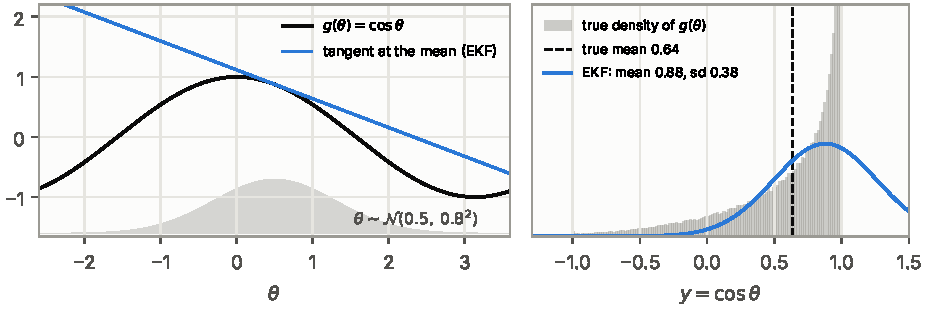
\includegraphics[width=\linewidth]{figures/ch04_linearisation.pdf}
\caption{Linearisation in one dimension. Left: $g(\theta)=\cos\theta$, the
input density (grey) and the tangent at its mean, which is all the EKF
uses. Right: the true density of $g(\theta)$ (histogram of $200\,000$
samples) and the EKF's Gaussian. The EKF's mean misses the curvature: it
is too high by $0.24$.}
\label{fig:linearisation}
\end{figure}

\Cref{fig:arc} shows the consequence. A mower known to within $1$ unit but
with a heading uncertainty of $\sigma_\theta=0.8$\,rad (about $45^\circ$)
drives 10 steps of 4 units straight ahead. The true distribution is an
arc. The EKF puts its mean at the tip of the arc, $11.05$ units ahead of
the true mean ($40(1-e^{-0.32})=10.95$ in theory), and its ellipse is a
needle, much too thin along the direction of travel.

\begin{figure}[ht]
\centering
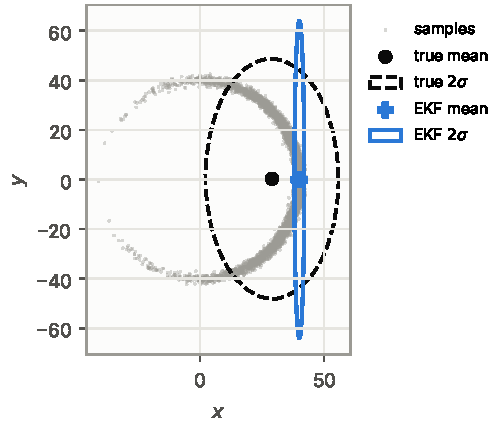
\includegraphics{figures/ch04_arc.pdf}
\caption{Forty units driven with a $45^\circ$ heading uncertainty. Grey:
5\,000 samples of the true distribution, with its mean and $2\sigma$
ellipse (dashed). Blue: the EKF's prediction, mean through $f$ and
covariance through $F$.}
\label{fig:arc}
\end{figure}

\section{Over-confidence}

Inside the filter, the same mechanism makes the EKF \emph{over-confident}
after an uncertain start. Twenty runs start from an estimate drawn from
$\Normal(\x_0,P_0)$ with $\sigma_{xy}=30$ and $\sigma_\theta=0.8$; the
sensor range is limited to 110 units, so that only one or two landmarks are
seen at a time. The average NEES (\cref{fig:ekftransient}) is $297$ after
the first update, $63$ after five and $6.5$ after twenty, against an
expected value of $3$.

\begin{figure}[ht]
\centering
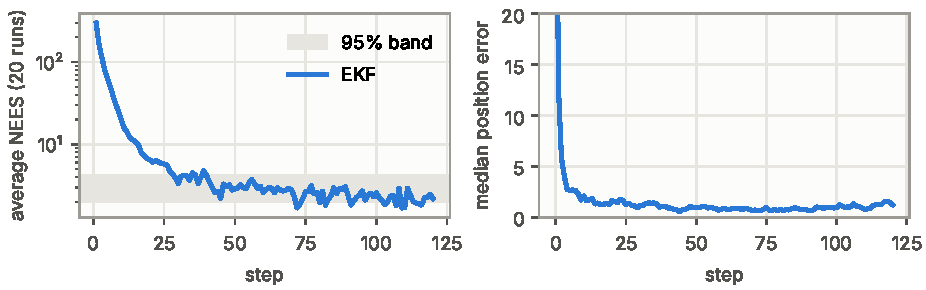
\includegraphics[width=\linewidth]{figures/ch04_transient.pdf}
\caption{EKF after an uncertain start (20 runs). Left: average NEES (log
scale) and the $95\%$ band for $n=3$. Right: median position error. The
filter converges, but for about twenty steps its covariance claims tens
to hundreds of times more precision than it has.}
\label{fig:ekftransient}
\end{figure}

The mechanism is easy to see. The Jacobian $H$ is evaluated at the
estimate $\bx$, which is tens of units and up to a radian away from the
truth. The update then treats the measurement as a linear function of the
state with \emph{that} slope, and $H\T R^{-1}H$ (\cref{prop:information})
adds information along directions computed at the wrong place. The
covariance shrinks as if the measurement had pinned the state down, while
the estimate has only moved part of the way. The next update, with a
small $\bar P$, then gives the new measurements little weight. If the error
had been larger, that false confidence could have made the filter reject
(by gating, \cref{sec:ekf-association}) the very measurements that would
have corrected it.

Common remedies: inflate $Q$ or $R$ while the uncertainty is large (cheap
and ad hoc); propagate the uncertainty without linearising (the UKF,
Chapter~\ref{ch:ukf}); or \emph{iterate} the update.

\section{The update as one Gauss--Newton step}

There is another way to look at the update. The posterior density is the
product of the predicted belief and the likelihood; its \emph{mode} is the
most probable pose. Maximising a product of Gaussian densities is the same
as minimising the sum of their exponents, a least-squares problem.
\emph{Gauss--Newton} is the standard method for non-linear least squares:
linearise the non-linear residual at the current point, solve the
resulting linear least-squares problem exactly, and repeat from the
solution.

\begin{proposition}{EKF and iterated EKF updates are Gauss--Newton steps}{gaussnewton}
The posterior mode of $\Normal(\x;\bx,\bar P)\,\Normal(\z;h(\x),R)$
minimises
\[
  J(\x)=\tfrac12\norm{\x-\bx}_{\bar P}^2+\tfrac12\norm{\z-h(\x)}_R^2,
  \qquad\norm{\vect{e}}_A^2=\vect{e}\T A^{-1}\vect{e}.
\]
One Gauss--Newton step on $J$ from $\x_i$, with $H_i=\partial h/\partial
\x(\x_i)$, gives
\begin{equation}\label{eq:iekf}
  \x_{i+1}=\bx+K_i\bigl(\z-h(\x_i)-H_i(\bx-\x_i)\bigr),\qquad
  K_i=\bar PH_i\T(H_i\bar PH_i\T+R)^{-1}.
\end{equation}
From $\x_0=\bx$, the first step is exactly the EKF update. Iterating to
convergence is the \emph{iterated} EKF.
\end{proposition}

\begin{proof}
Gauss--Newton linearises the residual $\z-h(\x)\approx\z-h(\x_i)-H_i
(\x-\x_i)$ and minimises the resulting quadratic. Its minimiser satisfies
$(\bar P^{-1}+H_i\T R^{-1}H_i)(\x-\bx)=H_i\T R^{-1}(\z-h(\x_i)-H_i(\bx-
\x_i))$, obtained by setting the gradient to zero. By
\cref{prop:information} the inverse of the left matrix is
$P_i=(I-K_iH_i)\bar P$ and $P_iH_i\T R^{-1}=K_i$, which gives
\eqref{eq:iekf}. With $\x_0=\bx$ the bracket is $\z-h(\bx)=\y$.
\end{proof}

\begin{inwords}
The EKF update is one step of an optimiser on the right cost function,
stopped after the first iteration. When the estimate is far from the
truth, one step is not enough; iterating, with re-linearisation at each
step, gets closer to the true posterior mode. This is also the bridge to
modern SLAM, which solves the same least-squares problem for a whole
trajectory at once (Chapter~\ref{ch:choosing}).
\end{inwords}

\section{Data association}
\label{sec:ekf-association}

So far the sensor has said which landmark it saw. When it does not, the
EKF must decide, before it can update, which landmark produced each
measurement $\z_k$. The standard choice is \emph{maximum-likelihood}
(nearest-neighbour) association: for each candidate $j$, compute the
innovation $\y_{kj}=\z_k-h_j(\bx)$ (bearing wrapped) and its covariance
$S_j=H_j\bar PH_j\T+R_1$, and choose
\[
  j^\star=\arg\min_j\;\y_{kj}\T S_j^{-1}\y_{kj}+\log\det S_j,
\]
the landmark under which the measurement is most likely. Indeed, if
landmark $j$ produced the measurement, the innovation is approximately
$\Normal(\vect0,S_j)$, and $-2\log\Normal(\y;\vect0,S)=\y\T S^{-1}\y+
\log\det S+\text{constant}$. The quantity $\y\T S^{-1}\y$ is the squared
\emph{Mahalanobis distance}: the size of the innovation counted in
standard deviations. For the right landmark and a consistent filter it
follows a $\chi^2_2$ distribution (this is the NIS of
\cref{ch:kalman}). A \emph{gate} therefore rejects the measurement when
even the best Mahalanobis distance exceeds a high quantile of $\chi^2_2$:
such a measurement is too surprising to come from any known landmark.

This works as long as the estimate is good. Once it is off by more than
about half the spacing between landmarks, the nearest landmark is the
wrong one. The update then pulls the estimate \emph{further} in the wrong
direction and shrinks its covariance, which makes the next wrong
association even more likely. In the showdown of
Chapter~\ref{ch:choosing}, an EKF with nearest-neighbour association loses
the mower in half of the uncertain starts and in six kidnappings out of
eight.

\begin{practice}[\nb{03\_extended\_kalman\_filter.ipynb}, \code{ekf.py}]
\code{motion\_jacobians} and \code{range\_bearing\_jacobian} implement
\cref{prop:jacobians}; \code{EKF} implements \cref{def:ekf} with the
Joseph update and \code{association="known"} or \code{"nearest"}. The
notebook checks the Jacobians by finite differences, plots the
$\pm2\sigma$ bands, and reproduces \cref{fig:arc,fig:ekftransient}.
\end{practice}

\begin{mower}
A mower is most uncertain when it matters most: after start-up, after a
long stretch without fixes (under a tree, along a wall), or after it has
been moved by hand. Those are exactly the moments when the EKF is
over-confident. A practical system watches the NIS of
\cref{ch:kalman}; when it leaves its band, the EKF is re-initialised from a
more robust estimator, for instance a particle filter or a GNSS fix.
\end{mower}

\section*{What to remember from this chapter}
\addcontentsline{toc}{section}{What to remember}

\begin{enumerate}[nosep]
  \item The EKF keeps a Gaussian belief on the full pose. The mean goes
    through the true models $f$ and $h$; the covariance goes through their
    Jacobians $F$, $V$ and $H$, evaluated at the current estimate.
  \item Linearisation ignores curvature. The mean of a curved function is
    not the function of the mean: the EKF's prediction is biased, by
    $\tfrac12\tr(\nabla^2g\,\Sigma)$ to leading order, and its covariance
    is too thin.
  \item When the uncertainty is small the EKF is accurate, honest and
    cheap. After a very uncertain start it is over-confident: the
    Jacobians are computed at the wrong place.
  \item The EKF update is one Gauss--Newton step on a least-squares cost;
    iterating it (the iterated EKF) gets closer to the posterior mode.
  \item With unidentified landmarks the EKF must choose one association
    per measurement. A wrong choice is reinforced by the update, and the
    filter can lose the mower for good.
\end{enumerate}

\FloatBarrier
\section*{Exercises}
\addcontentsline{toc}{section}{Exercises}

\begin{enumerate}[label=\textbf{4.\arabic*},ref=4.\arabic*]
\item\label{ex:ekfexact} Show that if $f$ and $h$ are affine, the EKF is
  exactly the Kalman filter.
\item\label{ex:cosvar} Let $\theta\sim\Normal(0,\sigma^2)$ and
  $y=\cos\theta$. What mean and variance does linearisation at $0$ give for
  $y$? Compute the true ones, and evaluate both for $\sigma=0.8$.
\item\label{ex:rangebias} Using \cref{prop:secondorder}, show that the mean
  of the range to a landmark is biased upwards by about
  $\sigma_\perp^2/(2r)$, where $\sigma_\perp^2$ is the position variance
  perpendicular to the line of sight. Why perpendicular?
\item\label{ex:gate} With a gate at the $99\%$ quantile of $\chi^2_2$,
  what fraction of correct measurements does a consistent EKF reject? And
  an EKF whose innovation covariance $S$ is ten times too small?
\end{enumerate}

\subsection*{Solutions}

\textbf{4.1.} If $f(\x,\uu)=F\x+B\uu+\vect{c}$, its Jacobian is $F$ and
the EKF predicted covariance is $FPF\T+Q$; if the noise enters through
the control as $f(\x,\uu+\bepsilon)$, it is affine in $\bepsilon$ too and
$VMV\T$ is the exact covariance of the noise term. The mean $f(\hx,\uu)$
is the exact mean by linearity. For an affine $h(\x)=H\x+\vect{c}$, the
innovation is $\z-H\bx-\vect{c}$ and the remaining formulas are those of
\cref{thm:kf}. Linearisation is exact for affine maps, so every step
coincides.

\textbf{4.2.} At $0$, $\cos'(0)=0$: linearisation gives
$y\approx1$, with mean $1$ and variance $0$. Exactly,
$\E[y]=e^{-\sigma^2/2}$ (Exercise~\ref{ex:ecos}) and
$\E[y^2]=\E[(1+\cos2\theta)/2]=(1+e^{-2\sigma^2})/2$, so
$\Var(y)=\tfrac12(1-e^{-\sigma^2})^2$. For $\sigma=0.8$: mean $0.726$
(not $1$) and standard deviation $0.334$ (not $0$). Linearising at a
stationary point loses \emph{all} the uncertainty; this is the needle of
\cref{fig:arc}.

\textbf{4.3.} For $r(\p)=\norm{\bell-\p}$, $\nabla r=-\hat{\vect{d}}$ and
$\nabla^2r=(I-\hat{\vect{d}}\hat{\vect{d}}\T)/r$ with
$\hat{\vect d}=\vect{d}/r$. So
$\tfrac12\tr(\nabla^2r\,\Sigma)=\tfrac1{2r}(\tr\Sigma-\hat{\vect{d}}\T
\Sigma\hat{\vect{d}})=\sigma_\perp^2/(2r)$. Moving along the line of sight
changes the range linearly (no curvature); moving perpendicular to it
always increases the range, by Pythagoras, so the errors do not average
out. The bias is small far from the landmark and large close to it.

\textbf{4.4.} For a consistent filter, the Mahalanobis distance of a
correct measurement is $\chi^2_2$, whose $99\%$ quantile is
$-2\log0.01=9.21$; $1\%$ of correct measurements are rejected. If $S$ is
ten times too small, the actual distance is ten times the
$\chi^2_2$ variable, and it exceeds $9.21$ with probability
$e^{-0.921/2}=0.63$: the filter rejects most of the measurements that
would correct it.

\chapter{The unscented Kalman filter}
\label{ch:ukf}

The EKF approximates the \emph{function} by a tangent plane and propagates
the Gaussian exactly through that approximation. The unscented Kalman
filter (UKF) does the opposite: it keeps the function exact and
approximates the \emph{distribution} by a handful of deterministically
chosen points, the \emph{sigma points}, then fits a Gaussian to where they
land. No Jacobian is needed, the mean is correct to one order higher, and,
as this chapter proves, the update automatically accounts for the
linearisation error that made the EKF over-confident.

\section{The unscented transform}

The problem is the one of \cref{prop:secondorder}: $X$ is Gaussian, $g$ is
non-linear, and we want the mean and the covariance of $g(X)$. The idea is
best seen in one dimension. Replace $\Normal(\mu,\sigma^2)$ by two points,
$\mu-\sigma$ and $\mu+\sigma$, each with weight $\tfrac12$. These two
points have the same mean and the same variance as the Gaussian. Apply $g$
to each, and take the mean and the variance of the two results. If $g$
bends, the two results are not symmetric about $g(\mu)$, and their average
moves away from it, as the true mean does.

In $n$ dimensions the same is done along $n$ directions, the columns of a
square root of the covariance, with a centre point added. The square root
used is the \emph{Cholesky factor} of $\Sigma$: the lower-triangular
matrix $L$ with $LL\T=\Sigma$, which exists and is unique (with a positive
diagonal) when $\Sigma$ is positive definite. Three parameters
tune the construction: $\alpha$ and $\kappa$ set how far from the mean the
points are placed, and $\beta$ adjusts the weight of the centre point in
the covariance.

\begin{definition}{Scaled sigma points}{sigma}
Let $\bmu\in\R^n$, $\Sigma\succ0$ with Cholesky factor $LL\T=\Sigma$
(columns $L_i$), and parameters $\alpha>0$, $\beta\ge0$, $\kappa$ with
$\lambda=\alpha^2(n+\kappa)-n>-n$. The $2n+1$ sigma points are
\[
  \chi_0=\bmu,\qquad\chi_{\pm i}=\bmu\pm\sqrt{n+\lambda}\,L_i,\quad
  i=1,\dots,n,
\]
with mean weights $W^{(m)}$ and covariance weights $W^{(c)}$:
\[
  W^{(m)}_0=\frac\lambda{n+\lambda},\quad
  W^{(c)}_0=W^{(m)}_0+1-\alpha^2+\beta,\quad
  W^{(m)}_{\pm i}=W^{(c)}_{\pm i}=\frac1{2(n+\lambda)}.
\]
The \emph{unscented transform} of $\Normal(\bmu,\Sigma)$ through $g$ is
\[
  \hat\y=\sum_jW^{(m)}_jg(\chi_j),\qquad
  P_y=\sum_jW^{(c)}_j\bigl(g(\chi_j)-\hat\y\bigr)
  \bigl(g(\chi_j)-\hat\y\bigr)\T .
\]
\end{definition}

\begin{figure}[ht]
\centering
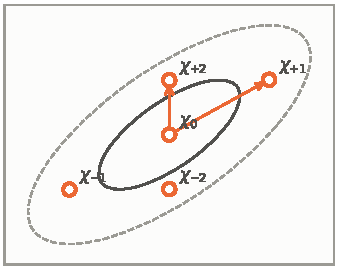
\includegraphics[width=0.45\linewidth]{figures/ch05_sigma_points.pdf}
\caption{The five sigma points of a two-dimensional Gaussian
($\alpha=1$, $\kappa=0$): the mean, and the mean $\pm\sqrt{n+\lambda}$
times each column of the Cholesky factor (arrows). Solid: the $1\sigma$
ellipse; dashed: $2\sigma$.}
\label{fig:sigmapoints}
\end{figure}

\Cref{fig:sigmapoints} shows the points for $n=2$. The columns $L_i$ of
the Cholesky factor play the role of $\sigma$ in one dimension: each is
one standard deviation of the Gaussian in one of $n$ independent
directions.

\begin{example}{The mean of a cosine}{utcos}
Take the example of \cref{fig:linearisation}: $\theta\sim\Normal(0.5,
0.8^2)$ and $g=\cos$. With the parameters used in this book ($\alpha=1$,
$\beta=2$, $\kappa=0$) and $n=1$, $\lambda=0$: the sigma points are $0.5$
and $0.5\pm0.8$, that is $-0.3$, $0.5$ and $1.3$, with mean weights
$\tfrac12$, $0$, $\tfrac12$. The unscented mean is
$\tfrac12(\cos(-0.3)+\cos1.3)=\tfrac12(0.955+0.267)=0.611$. The true mean
is $e^{-0.32}\cos0.5=0.637$, and linearisation gives $\cos0.5=0.878$.
The error falls from $0.878-0.637=0.241$ to $0.637-0.611=0.026$: two
evaluations of the function have removed nine tenths of it.
\end{example}

\begin{proposition}{Sigma points match the first two moments}{moments}
$\sum_jW^{(m)}_j=1$, $\sum_jW^{(m)}_j\chi_j=\bmu$ and
$\sum_jW^{(c)}_j(\chi_j-\bmu)(\chi_j-\bmu)\T=\Sigma$, and the same holds
with the mean weights $W^{(m)}_j$. All odd central moments of the weighted
points vanish.
\end{proposition}

\begin{proof}
Write $\vect\delta_j=\chi_j-\bmu$ for the offset of each point:
$\vect\delta_0=\vect0$ and $\vect\delta_{\pm i}=\pm\sqrt{n+\lambda}\,L_i$.

\emph{The weights add up to $1$.} The centre has the weight
$\lambda/(n+\lambda)$, and the $2n$ other points have
$1/(2(n+\lambda))$ each:
\[
  \sum_jW^{(m)}_j=\frac{\lambda}{n+\lambda}+2n\cdot\frac1{2(n+\lambda)}
  =\frac{\lambda+n}{n+\lambda}=1 .
\]

\emph{Odd moments vanish.} The points $\chi_{+i}$ and $\chi_{-i}$ have the
same weight and opposite offsets, so in any sum of an odd power of the
offsets (for instance $\sum_jW_j\vect\delta_j$, or
$\sum_jW_j\,\delta_{j,a}\delta_{j,b}\delta_{j,c}$ for three coordinates)
their two contributions cancel. The centre, with $\vect\delta_0=\vect0$,
contributes nothing to any central moment, whatever its weight.

\emph{The mean.} Then
$\sum_jW^{(m)}_j\chi_j=\bmu\sum_jW^{(m)}_j+\sum_jW^{(m)}_j\vect\delta_j
=\bmu\times1+\vect0=\bmu$.

\emph{The covariance.} The centre contributes nothing, and the two points
$\chi_{\pm i}$ have the same weight in both families of weights, so both
sums equal
\[
  \sum_{i=1}^n2\cdot\frac{1}{2(n+\lambda)}\,(n+\lambda)L_iL_i\T
  =\sum_{i=1}^nL_iL_i\T=LL\T=\Sigma,
\]
because $\vect\delta_{\pm i}\vect\delta_{\pm i}\T=(n+\lambda)L_iL_i\T$,
and a matrix times its transpose is the sum of the products of its
columns, $LL\T=\sum_iL_iL_i\T$.
\end{proof}

\begin{theorem}{The unscented mean is exact up to third order}{utorder}
Let $X\sim\Normal(\bmu,\Sigma)$. If every component of $g$ is a
polynomial of degree at most $3$, then $\hat\y=\E[g(X)]$. For a smooth
$g$ with bounded fourth derivatives, $\hat\y-\E[g(X)]=O(\norm\Sigma^2)$,
whereas the linearised mean $g(\bmu)$ has an error of order
$\norm\Sigma$ (\cref{prop:secondorder}).
\end{theorem}

\begin{proof}
Compare, term by term, the Taylor expansion of $g_i$ around $\bmu$
averaged in two ways: over $X$ (the true mean) and over the weighted
sigma points (the unscented mean). With $\vect\delta$ the offset from
$\bmu$ ($\vect e=X-\bmu$ for $X$, $\vect\delta_j=\chi_j-\bmu$ for the
points),
\[
  g_i(\bmu+\vect\delta)=g_i(\bmu)+\nabla g_i\T\vect\delta
  +\tfrac12\vect\delta\T\nabla^2g_i\,\vect\delta
  +\tfrac16D^3g_i[\vect\delta,\vect\delta,\vect\delta]+\rho(\vect\delta).
\]
\begin{itemize}[nosep]
  \item \emph{Constant term.} $g_i(\bmu)$ on both sides, since both sets of
        weights add up to $1$.
  \item \emph{First- and third-order terms.} Zero on both sides: for $X$
        because the odd moments of a centred Gaussian are zero (proof of
        \cref{prop:secondorder}), for the sigma points by
        \cref{prop:moments}.
  \item \emph{Second-order term.} $\tfrac12\tr(\nabla^2g_i\Sigma)$ on both
        sides. For $X$ this is the proof of \cref{prop:secondorder}. For
        the points, with the trace identity used there and
        \cref{prop:moments},
        \[
          \sum_jW^{(m)}_j\tfrac12\vect\delta_j\T\nabla^2g_i\vect\delta_j
          =\tfrac12\tr\Bigl(\nabla^2g_i\sum_jW^{(m)}_j\vect\delta_j
          \vect\delta_j\T\Bigr)=\tfrac12\tr(\nabla^2g_i\Sigma).
        \]
\end{itemize}
For a polynomial of degree at most $3$ there is no remainder $\rho$, so
the two means coincide. Otherwise each side
keeps a fourth-order remainder: $O(\norm\Sigma^2)$ for $X$ (proof of
\cref{prop:secondorder}), and at most $C\norm{\vect\delta_j}^4\le
C(n+\lambda)^2\norm\Sigma^2$ at each sigma point, since
$\norm{L_i}^2\le\norm\Sigma$. The two means therefore differ by
$O(\norm\Sigma^2)$.
\end{proof}

\begin{inwords}
Seven points (in three dimensions) are enough to capture the curvature
term that the EKF misses. The UKF does not differentiate anything: it
simply evaluates the model at well-placed points and lets the model's own
curvature show up in the results.
\end{inwords}

The covariance $P_y$ is correct to first order, like the EKF's, and
captures part of the higher-order terms; $\beta$ adds information about
the fourth moment. (These statements are not proved here; see Julier and
Uhlmann, and Wan and van der Merwe, in the references. The next example
can be checked by hand.) For $y=x^2$ with $x\sim\Normal(\mu,\sigma^2)$, the
choice $\alpha=1$, $\beta=2$, $\kappa=0$ gives both the mean
$\mu^2+\sigma^2$ and the variance $4\mu^2\sigma^2+2\sigma^4$
\emph{exactly}, where linearisation gives $\mu^2$ and $4\mu^2\sigma^2$
(Exercise~\ref{ex:square}).

\paragraph{Choosing the parameters.} The original choice $\lambda=3-n$
($\alpha=1$, $\kappa=3-n$, $\beta=0$) matches the Gaussian kurtosis (the
fourth moment, $3\sigma^4$) along each axis (Exercise~\ref{ex:kurtosis}), but makes the centre weight
$W_0=(3-n)/3$ \emph{negative} as soon as $n>3$. A negative weight in a
covariance can produce an indefinite $P_y$ (Exercise~\ref{ex:negative}),
after which the next Cholesky factorisation fails. This book uses
$\alpha=1$, $\beta=2$, $\kappa=0$, so that $\lambda=0$, $W^{(m)}_0=0$ and
$W^{(c)}_0=2$: every covariance weight is non-negative.

\Cref{fig:utarc} replays the arc of \cref{fig:arc} with the unscented
transform. The exact mean is $(40e^{-0.32},0)=(29.05,0)$ (Exercise
\ref{ex:ecos}); the UKF's mean is $0.08$ units from it, the EKF's about
$11$. The UKF's ellipse covers the arc, but it is too wide along the
direction of travel (standard deviation $21.8$ against $13.4$) and
slightly too narrow across it ($22.7$ against $24.1$). Notebook~04
computes these exact values from Exercises~\ref{ex:ecos}
and~\ref{ex:cosvar} and compares. Neither can represent the arc itself: both summarise
it by a Gaussian.

\begin{figure}[ht]
\centering
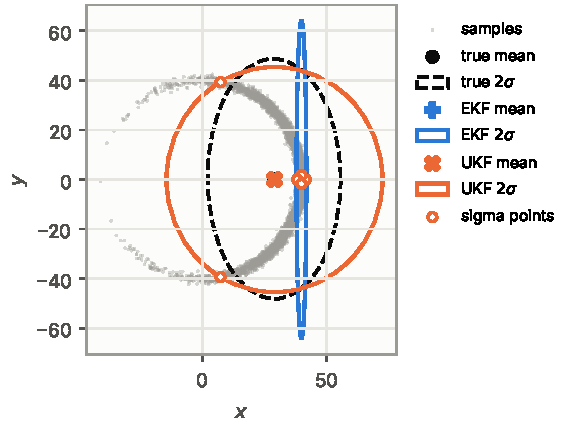
\includegraphics{figures/ch05_arc.pdf}
\caption{The arc of \cref{fig:arc}: forty units driven with a $45^\circ$ heading
uncertainty. Grey: $5\,000$ samples of the true distribution, with its
mean and $2\sigma$ ellipse (dashed). Blue: the EKF's prediction. Orange:
the unscented transform, with its seven transformed sigma points.}
\label{fig:utarc}
\end{figure}

\section{The filter}

The filter uses the unscented transform twice per cycle: through the
motion model $f$ for the prediction, and through the sensor model $h$ for
the update.

\paragraph{Non-additive noise.} The control noise acts inside the motion
model, $f(\x,\uu+\bepsilon)$: the turn error is applied before the robot
drives. It enters $f$ non-linearly and cannot simply be added as a $Q$.
The standard remedy is to \emph{augment} the state with the noise,
\[
  \x^a=\begin{pmatrix}\x\\\bepsilon\end{pmatrix}\sim
  \Normal\left(\begin{pmatrix}\hx\\\vect0\end{pmatrix},
  \begin{pmatrix}P&0\\0&M\end{pmatrix}\right),\qquad n_a=3+2=5,
\]
draw $2n_a+1=11$ sigma points and push each through
$f(\x,\uu+\bepsilon)$. Each augmented sigma point $\chi^a_j$ has five
components: the first three, written $\chi^x_j$, are a pose, and the last
two, written $\chi^\varepsilon_j$, are a control noise. The measurement
noise is additive and does not need augmentation.

\paragraph{The update.} The prediction gives a new Gaussian
$\Normal(\bx,\bar P)$, so new sigma points $\chi_j$ are drawn from it,
seven of them. Pushing them through the sensor model, $Z_j=h(\chi_j)$,
gives sigma-point estimates of three quantities: the predicted measurement
$\hat\z$, the covariance $S$ of the measurement (to which the sensor noise
$R$ is added), and the cross-covariance $P_{xz}=\Cov(\x,\z)$ between the
pose and the measurement. The update is then \cref{thm:conditioning},
applied as if $(\x,\z)$ were jointly Gaussian with these moments: the gain
is $\Sigma_{xy}\Sigma_{yy}^{-1}=P_{xz}S^{-1}$, and the covariance decreases
by $\Sigma_{xy}\Sigma_{yy}^{-1}\Sigma_{yx}=P_{xz}S^{-1}P_{xz}\T
=(P_{xz}S^{-1})S(P_{xz}S^{-1})\T=KSK\T$.

\begin{definition}{Unscented Kalman filter}{ukf}
\emph{Predict}: sigma points $\chi^a_j$ of the augmented Gaussian;
$\chi'_j=f(\chi^x_j,\uu+\chi^\varepsilon_j)$; $(\bx,\bar P)$ is the
unscented transform of these points.

\emph{Update}: fresh sigma points $\chi_j$ of $\Normal(\bx,\bar P)$;
$Z_j=h(\chi_j)$;
\begin{gather*}
  \hat\z=\sum_jW^{(m)}_jZ_j,\qquad
  S=\sum_jW^{(c)}_j(Z_j-\hat\z)(Z_j-\hat\z)\T+R,\\
  P_{xz}=\sum_jW^{(c)}_j(\chi_j-\bx)(Z_j-\hat\z)\T,\qquad
  K=P_{xz}S^{-1},\\
  \hx=\bx+K(\z-\hat\z),\qquad P=\bar P-KSK\T .
\end{gather*}
Heading and bearing components are averaged on the circle and every
residual is wrapped (\cref{sec:ukf-angles}).
\end{definition}

For a linear $h(\x)=H\x$ these are $P_{xz}=\bar PH\T$ and
$S=H\bar PH\T+R$: by \cref{prop:moments}, $\hat\z=H\bx$, so
$Z_j-\hat\z=H(\chi_j-\bx)$, and the sums become
$\bigl(\sum_jW^{(c)}_j(\chi_j-\bx)(\chi_j-\bx)\T\bigr)H\T=\bar PH\T$ and
$H\bar PH\T$. The update is then exactly the Kalman update of
\cref{thm:kf}. In general it is
that update with $\bar PH\T$ and $H\bar PH\T+R$ replaced by their
sigma-point estimates. What does that replacement do?

\Cref{fig:regression} shows it in one dimension. The EKF replaces $h$ by
its tangent at the mean. The UKF never computes a slope, but its update
behaves as if $h$ had been replaced by another straight line: the one that
fits the values of $h$ at the sigma points best, in the least-squares
sense: among the lines through $(\bx,\hat\z)$, the one with the slope $A$
that minimises $\sum_jW^{(c)}_j\norm{Z_j-\hat\z-A(\chi_j-\bx)}^2$. This is a \emph{regression} line, and its slope is
$\Cov(\z,\x)\Cov(\x)^{-1}$, the regression coefficient already met in
\cref{thm:conditioning}; here it is $\tilde H=P_{xz}\T\bar P^{-1}$. To see
it, write $\vect\delta_j=\chi_j-\bx$. With non-negative weights the sum
is a convex quadratic in $A$, so its minimum is where its derivative with
respect to $A$ vanishes:
\[
  \sum_jW^{(c)}_j\bigl(Z_j-\hat\z-A\vect\delta_j\bigr)\vect\delta_j\T=0,
  \qquad\text{that is}\qquad
  \underbrace{\sum_jW^{(c)}_j(Z_j-\hat\z)\vect\delta_j\T}_{P_{xz}\T}
  =A\underbrace{\sum_jW^{(c)}_j\vect\delta_j\vect\delta_j\T}_{\bar P},
\]
the second sum being $\bar P$ by \cref{prop:moments}. So
$A=P_{xz}\T\bar P^{-1}$. Because
$h$ is curved, the sigma points do not lie exactly on that line. Their
scatter around it is what a straight line cannot explain, and the UKF
counts it as extra measurement noise. The next theorem states this
precisely; ``statistically linearised'' is the usual name for a slope
obtained by regression instead of differentiation.

\begin{figure}[ht]
\centering
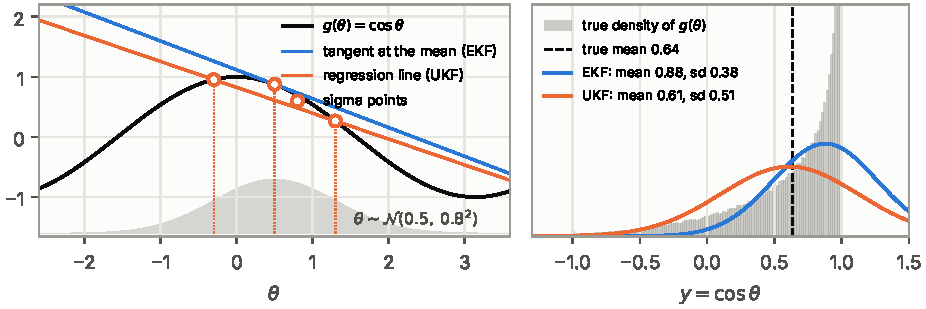
\includegraphics[width=\linewidth]{figures/ch05_regression.pdf}
\caption{The example of \cref{fig:linearisation}, with the unscented transform
added: an angle $\theta\sim\Normal(0.5,0.8^2)$ (grey density, left) is
passed through $\cos$. The UKF evaluates $\cos$ at three sigma points and fits a
regression line through them (slope $\tilde H=-0.43$; the tangent's is
$-0.48$). The two outer points lie on that line; the centre point is off
it by $0.27$, and the weighted scatter, $\Omega=0.14$, is added to the
output variance. The UKF's mean ($0.61$) is
close to the true mean ($0.64$), and its spread covers the true
distribution.}
\label{fig:regression}
\end{figure}

\begin{theorem}{The UKF update is a Kalman update with an inflated $R$}{slr}
Assume all $W^{(c)}_j\ge0$. Define the \emph{statistically linearised}
measurement matrix $\tilde H=P_{xz}\T\bar P^{-1}$ and the residuals
$\vect\zeta_j=Z_j-\hat\z-\tilde H(\chi_j-\bx)$. Then
\[
  P_{xz}=\bar P\tilde H\T,\qquad
  S=\tilde H\bar P\tilde H\T+R+\Omega,\qquad
  \Omega=\sum_jW^{(c)}_j\vect\zeta_j\vect\zeta_j\T\succeq0,
\]
so the UKF update is the Kalman update for the affine model
$\z=\hat\z+\tilde H(\x-\bx)+\vv'$ with noise covariance
$R+\Omega\succeq R$.
\end{theorem}

\begin{proof}
\emph{The cross-covariance.} From $\tilde H=P_{xz}\T\bar P^{-1}$,
$\tilde H\T=\bar P^{-1}P_{xz}$ ($\bar P$ is symmetric), so
$\bar P\tilde H\T=P_{xz}$.

\emph{The residuals are uncorrelated with the offsets.} Write
$\vect\delta_j=\chi_j-\bx$, so that
$Z_j-\hat\z=\tilde H\vect\delta_j+\vect\zeta_j$ by the definition of
$\vect\zeta_j$. Then
\[
  \sum_jW^{(c)}_j\vect\zeta_j\vect\delta_j\T
  =\sum_jW^{(c)}_j(Z_j-\hat\z)\vect\delta_j\T
   -\tilde H\sum_jW^{(c)}_j\vect\delta_j\vect\delta_j\T
  =P_{xz}\T-\tilde H\bar P=0 ,
\]
using \cref{prop:moments} for the second sum and the first step for the
last equality.

\emph{The innovation covariance.} By the definition of $S$ and the same
decomposition,
\begin{align*}
  S-R&=\sum_jW^{(c)}_j(\tilde H\vect\delta_j+\vect\zeta_j)
       (\tilde H\vect\delta_j+\vect\zeta_j)\T\\
  &=\tilde H\Bigl(\sum_jW^{(c)}_j\vect\delta_j\vect\delta_j\T\Bigr)\tilde H\T
   +\tilde H\sum_jW^{(c)}_j\vect\delta_j\vect\zeta_j\T
   +\sum_jW^{(c)}_j\vect\zeta_j\vect\delta_j\T\tilde H\T
   +\sum_jW^{(c)}_j\vect\zeta_j\vect\zeta_j\T\\
  &=\tilde H\bar P\tilde H\T+0+0+\Omega .
\end{align*}
$\Omega$ is a combination, with non-negative weights, of the positive
semi-definite matrices $\vect\zeta_j\vect\zeta_j\T$, hence positive
semi-definite.

\emph{The equivalent Kalman update.} The affine model of the statement
has the cross-covariance $\Cov(\x,\tilde H\x+\vv')=\bar P\tilde H\T=
P_{xz}$ and the innovation covariance $\tilde H\bar P\tilde H\T+R+\Omega=
S$. Its Kalman gain $P_{xz}S^{-1}$ and its updated covariance
$\bar P-KSK\T$ are therefore those of the UKF.
\end{proof}

\begin{inwords}
The UKF fits the best straight line to $h$ over the sigma points (a
weighted least-squares regression, not a tangent at one point), and
whatever that line cannot explain is added to the measurement noise. When
$h$ is nearly linear over the uncertainty, $\Omega\approx0$ and the UKF is
the EKF. When it is not, the UKF trusts the measurement less, exactly
where the EKF trusted it too much. This is why it is much less
over-confident after an uncertain start (\cref{fig:ukftransient}).
\end{inwords}


\section{Angles in the UKF}
\label{sec:ukf-angles}

Two components of the state and of the measurement are angles: the
heading, and the bearing of each landmark. They need care at two places.

\emph{Means.} The unscented transform averages the sigma points with the
weights $W^{(m)}_j$. For an angle component the plain average can point
the wrong way when the points straddle the cut at $\pm\pi$, so these
components are averaged with the circular mean of \cref{sec:circular}
instead (with the weights of this book, every $W^{(m)}_j$ is
non-negative).

\emph{Differences.} The same care is needed in the covariances. $P_y$,
$P_{xz}$ and the innovation are built from differences between an angle
and a mean angle, $\theta_j-\bar\theta$, and such a difference can be off
by $\pm2\pi$ (\cref{lem:wrap}). With $\theta_j=3.1$ and
$\bar\theta=-3.13$, the plain difference is $6.23$ where the rotation is
$-0.05$, and its square, $38.8$ instead of $0.0028$, would make the
covariance absurd. So every difference of angles is wrapped before it
enters a covariance or an innovation.

\section{Where the UKF earns its keep}

With four landmarks in view and a good start, the UKF and the EKF are
indistinguishable on the standard run (RMSE $0.99$ against $1.01$,
notebook~04): the models are nearly linear over the small uncertainty.
The UKF costs about 50\% more per step ($0.15$ against $0.10$\,ms in the
comparison of \cref{ch:choosing}, notebook~06; the exact figures depend
on the machine), for
$11+7$ model evaluations and two Cholesky factorisations instead of two
Jacobians.

After the uncertain start of \cref{fig:ekftransient}, however, the two
filters differ sharply (\cref{fig:ukftransient}). With the same runs and
the same initial estimates, the UKF's average NEES is $12$ after the first
update, $3.0$ after five and $2.9$ after twenty (EKF: $297$, $63$, $6.5$;
notebook~04 prints both), and its error drops slightly faster.

\begin{figure}[ht]
\centering
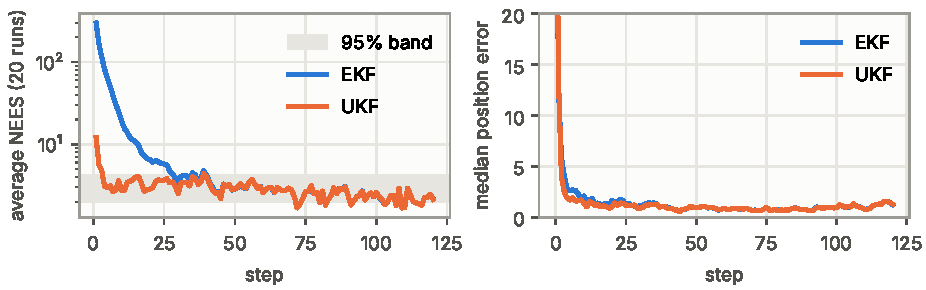
\includegraphics[width=\linewidth]{figures/ch05_transient.pdf}
\caption{The uncertain start of \cref{fig:ekftransient}, with both filters on the
same $20$ runs: the initial estimate is drawn from $\Normal(\x_0,P_0)$
with $\sigma_{xy}=30$ and $\sigma_\theta=0.8$. Left: average NEES (log
scale) and its $95\%$ band for $n=3$. Right: median position error. The UKF is within the band after a few
updates; the EKF is over-confident by up to two orders of magnitude.}
\label{fig:ukftransient}
\end{figure}

\begin{practice}[\nb{04\_unscented\_kalman\_filter.ipynb}, \code{ukf.py}]
\code{merwe\_weights}, \code{sigma\_points} and \code{unscented\_transform}
implement \cref{def:sigma}; \code{pose\_mean}, \code{meas\_mean} and the
residual functions handle the angles. \code{UKF} augments the state with
the control noise for the prediction and regenerates seven sigma points
for each update. A unit test checks that the transform is exact for
linear maps for several $(\alpha,\kappa)$, the cheapest possible guard
against the classic sigma-point bugs (a missing point, a spread of
$n+\lambda$ instead of $\sqrt{n+\lambda}$). The notebook reproduces
\cref{fig:utarc,fig:ukftransient}.
\end{practice}

\begin{mower}
The UKF is attractive whenever the Jacobians are tedious or error-prone:
with a camera model, an IMU on a chassis that pitches and rolls, or GNSS
antenna lever arms. Its cost grows with the number of sigma points,
linearly in the state dimension, and each point needs one evaluation of
the models; for the few-dimensional state of a mower this is negligible.
\end{mower}

\section*{What to remember from this chapter}
\addcontentsline{toc}{section}{What to remember}

\begin{enumerate}[nosep]
  \item The unscented transform replaces a Gaussian by $2n+1$ weighted
    points with the same mean and covariance, pushes them through the
    exact non-linear function, and fits a Gaussian to the results. No
    Jacobian is needed.
  \item Its mean is exact for polynomials up to degree $3$: it captures
    the curvature term that the EKF misses.
  \item The UKF is a Kalman filter in which the predicted mean and
    covariance, the innovation covariance $S$ and the cross-covariance
    $P_{xz}$ are computed from sigma points. The control noise is handled
    by augmenting the state.
  \item Its update is a Kalman update with the regression slope $\tilde H$
    and an inflated noise $R+\Omega$: what a straight line cannot explain
    is counted as noise. This keeps the UKF consistent where the EKF is
    over-confident.
  \item Angles need care: headings and bearings are averaged with the
    circular mean, and every residual is wrapped.
  \item The covariance weights must be non-negative, or the computed
    covariances may fail to be positive semi-definite; the parameters
    $\alpha=1$, $\beta=2$, $\kappa=0$ guarantee it.
\end{enumerate}

\FloatBarrier
\section*{Exercises}
\addcontentsline{toc}{section}{Exercises}

\begin{enumerate}[label=\textbf{5.\arabic*},ref=5.\arabic*]
\item\label{ex:square} Let $x\sim\Normal(\mu,\sigma^2)$ and $y=x^2$.
  Compute the unscented mean and variance of $y$ for $n=1$ and general
  $\lambda$, $W^{(c)}_0$. Show that they are exact if and only if
  $W^{(c)}_0+(n+\lambda-1)^2/(n+\lambda)=2$, and check the choice of this
  book.
\item\label{ex:kurtosis} For $n=1$, show that the sigma points with
  $n+\kappa=3$ (and $\alpha=1$) reproduce the fourth moment $3\sigma^4$ of
  a Gaussian.
\item\label{ex:negative} Take $\lambda=3-n$ with $n=5$ and $\beta=0$, so
  $W^{(c)}_0=W^{(m)}_0=w<0$. Let $g$ take one value $a$ at $\chi_0$ and
  another value $b$ at every other sigma point. Show that the unscented
  variance is $(a-b)^2w(1-w)<0$.
\end{enumerate}

\subsection*{Solutions}

\solution{5.1} \emph{The sigma points.} For $n=1$, write $c^2=n+\lambda
=1+\lambda$. By \cref{def:sigma} the points are $\mu$ and $\mu\pm c\sigma$;
the outer points have the weight $1/(2c^2)$ each, and the centre has the
mean weight $W^{(m)}_0=1-2\cdot\frac1{2c^2}=1-1/c^2$ and the covariance
weight $W^{(c)}_0$. The values of $y=x^2$ are
\[
  y_0=\mu^2,\qquad y_\pm=(\mu\pm c\sigma)^2=\mu^2\pm2\mu c\sigma+c^2\sigma^2 .
\]

\emph{The unscented mean.} In the sum $y_++y_-$ the terms $\pm2\mu c\sigma$
cancel:
\[
  \hat y=W^{(m)}_0\mu^2+\frac1{2c^2}\bigl(2\mu^2+2c^2\sigma^2\bigr)
  =\Bigl(W^{(m)}_0+\frac1{c^2}\Bigr)\mu^2+\sigma^2=\mu^2+\sigma^2 ,
\]
exact for any parameters, as \cref{thm:utorder} says for a polynomial of
degree $2$.

\emph{The unscented variance.} The deviations from $\hat y$ are
$y_0-\hat y=-\sigma^2$ at the centre and
$y_\pm-\hat y=\pm2\mu c\sigma+(c^2-1)\sigma^2$ at the others. Squaring,
\[
  (y_\pm-\hat y)^2=4\mu^2c^2\sigma^2\pm4\mu c\sigma(c^2-1)\sigma^2
  +(c^2-1)^2\sigma^4 ,
\]
and in the sum of the two the middle terms cancel. With the weights,
\[
  P_y=W^{(c)}_0\sigma^4+\frac1{2c^2}\cdot2\bigl(4\mu^2c^2\sigma^2
  +(c^2-1)^2\sigma^4\bigr)
  =4\mu^2\sigma^2+\Bigl(W^{(c)}_0+\frac{(c^2-1)^2}{c^2}\Bigr)\sigma^4.
\]

\emph{The true variance.} Write $x=\mu+e$ with $e\sim\Normal(0,\sigma^2)$.
Then $x^2=\mu^2+2\mu e+e^2$ and $\E[x^2]=\mu^2+\sigma^2$, so
$x^2-\E[x^2]=2\mu e+(e^2-\sigma^2)$, and
\begin{align*}
  \Var(x^2)&=\E\bigl[(2\mu e+e^2-\sigma^2)^2\bigr]
  =4\mu^2\E[e^2]+4\mu\,\E\bigl[e(e^2-\sigma^2)\bigr]
   +\E\bigl[(e^2-\sigma^2)^2\bigr]\\
  &=4\mu^2\sigma^2+0+\bigl(\E[e^4]-2\sigma^2\E[e^2]+\sigma^4\bigr)
  =4\mu^2\sigma^2+(3\sigma^4-2\sigma^4+\sigma^4)
  =4\mu^2\sigma^2+2\sigma^4,
\end{align*}
using $\E[e^3]=\E[e]=0$ (symmetry) and $\E[e^4]=3\sigma^4$
(\cref{ex:gaussmoments}).

\emph{When they agree.} The $\mu^2$ terms always agree, and the
$\sigma^4$ terms agree exactly when $W^{(c)}_0+(c^2-1)^2/c^2=2$. With the
choice of this book, $\alpha=1$, $\beta=2$, $\kappa=0$: $\lambda=0$, so
$c^2=1$, $W^{(m)}_0=0$ and $W^{(c)}_0=0+1-1+2=2$, and
$2+0=2$: exact. (With $\kappa=2$ and $\beta=2$, $c^2=3$ and
$W^{(c)}_0=\frac23+2=\frac83$, so $\frac83+\frac43=4$: the quartic term
is $4\sigma^4$, twice too much.)

\solution{5.2} With $\alpha=1$, $\lambda=\alpha^2(n+\kappa)-n=\kappa$, so
$n+\lambda=n+\kappa=3$, and the outer points are
$\mu\pm\sqrt{n+\lambda}\,\sigma=\mu\pm\sqrt3\,\sigma$. They have the weight
$\frac1{2(n+\lambda)}=\frac16$ each, and the centre adds nothing to a
central moment, so
\[
  \sum_jW_j(\chi_j-\mu)^4=2\cdot\frac16\cdot(\sqrt3\,\sigma)^4
  =\frac13\cdot9\sigma^4=3\sigma^4,
\]
the fourth moment of $\Normal(\mu,\sigma^2)$ (\cref{ex:gaussmoments}).
For larger $n$ the same holds along each axis of the Cholesky factor, but
the cross moments, such as $\E[e_1^2e_2^2]$, do not match.

\solution{5.3} \emph{The weight.} With $n=5$ and $\lambda=3-n=-2$, the
centre has the weight $w=\lambda/(n+\lambda)=-2/3$, and since $\beta=0$
and $\alpha=1$, $W^{(c)}_0=w+1-1+0=w$. The other ten points share the
weight $1-w$.

\emph{The mean.} $\hat y=wa+(1-w)b$.

\emph{The deviations.} At the centre, $a-\hat y=(1-w)a-(1-w)b
=(1-w)(a-b)$; at the other points, $b-\hat y=-w(a-b)$.

\emph{The variance.}
\[
  P_y=w\bigl((1-w)(a-b)\bigr)^2+(1-w)\bigl(w(a-b)\bigr)^2
  =(a-b)^2w(1-w)\bigl[(1-w)+w\bigr]=(a-b)^2w(1-w),
\]
which is negative when $w<0$. For $n=5$, $w(1-w)=-\frac23\cdot\frac53
=-\frac{10}9$, and $P_y=-\frac{10}9(a-b)^2$: a ``variance'' that is
negative.

\part{Sampling and synthesis}
\chapter{The particle filter}
\label{ch:particle}

The grid of Chapter~\ref{ch:bayes} stored the belief everywhere; the
Kalman filters assumed it was Gaussian. A \emph{particle filter} stores it
as a cloud of weighted samples,
\[
  \bel(\x_t)\approx\sum_{i=1}^Nw_t^{(i)}\,\delta_{\x_t^{(i)}},\qquad
  \sum_iw_t^{(i)}=1,
\]
where $\delta_{\x}$ denotes a point mass at $\x$: the formula says that the
pose is $\x_t^{(i)}$ with probability $w_t^{(i)}$. The average of any
function $\varphi$ of the pose under the belief is then approximated by
the weighted sum $\sum_iw_t^{(i)}\varphi(\x_t^{(i)})$. The filter puts its
effort where the probability is. The cloud can take any shape
(arcs, several separate bumps) and the models are used as they are,
without linearisation; the motion model only needs to be \emph{sampled},
which suits its degenerate transition (\cref{prop:degenerate}). Applied to
robot localisation this is \emph{Monte Carlo localisation}. This chapter
derives it from importance sampling, then studies its three failure
modes---weight degeneracy, sample impoverishment and mode collapse---and
the standard remedies.

\section{Importance sampling}

The particle filter rests on one idea. We want averages under a
distribution $\pi$ (the belief) from which we cannot sample directly, but
we can sample from another distribution $q$. When both have densities,
\[
  \E_\pi[\varphi]=\int\varphi(x)\,\pi(x)\,\mathrm dx
  =\int\varphi(x)\,\frac{\pi(x)}{q(x)}\,q(x)\,\mathrm dx
  =\E_q\Bigl[\varphi\,\frac\pi q\Bigr].
\]
So an average under $\pi$ is an average under $q$ in which each sample $x$
counts with the \emph{weight} $\pi(x)/q(x)$: more where $q$ proposes too
rarely, less where it proposes too often. In a filter, $\pi$ is known only
up to its normalising constant (the $\eta$ of \cref{thm:bayes}); dividing
the weights by their sum removes the need for it.

\begin{example}{Two outcomes}{istwo}
A target gives probability $0.2$ to $a$ and $0.8$ to $b$; the proposal
gives $0.5$ to each. The weights are $\pi/q=0.4$ for $a$ and $1.6$ for $b$.
Let $\varphi(a)=0$ and $\varphi(b)=10$, so that $\E_\pi[\varphi]=8$.
Suppose ten draws from the proposal give $a$ six times and $b$ four times.
The plain average of $\varphi$ over the draws is $4$, far from $8$. The
weights of the ten draws sum to $6\times0.4+4\times1.6=8.8$, and the
weighted average, with the weights divided by their sum, is
$(4\times1.6\times10)/8.8=7.3$: the weights have corrected
most of the mismatch between proposal and target, and the rest is sampling
noise, which vanishes as the number of draws grows.
\end{example}

\Cref{fig:importance} shows the same idea with continuous distributions.
The definition below is stated for general distributions; with densities,
$\mathrm d\pi/\mathrm dq$ is simply the ratio $\pi(x)/q(x)$.

\begin{definition}{Importance sampling}{is}
Let $\pi$ be a target distribution and $q$ a \emph{proposal} with
$\pi\ll q$ (every set of $q$-probability zero has $\pi$-probability
zero), and let $\tilde w=\mathrm d\pi/\mathrm dq$ be known up to a
constant: $\tilde w\propto w$. With $X^{(1)},\dots,X^{(N)}$ drawn
independently from $q$, the \emph{self-normalised} importance-sampling estimate of
$\E_\pi[\varphi]$ is
\[
  \hat\varphi_N=\sum_{i=1}^Nw^{(i)}\varphi(X^{(i)}),\qquad
  w^{(i)}=\frac{w(X^{(i)})}{\sum_kw(X^{(k)})}.
\]
\end{definition}

\begin{proposition}{Consistency}{isconsistent}
If $\E_\pi|\varphi|<\infty$, then $\hat\varphi_N\to\E_\pi[\varphi]$
almost surely as $N\to\infty$. If the normalising constant is known, the
unnormalised estimate $\frac1N\sum_i\tilde w(X^{(i)})\varphi(X^{(i)})$ is
moreover unbiased.
\end{proposition}

\begin{proof}
Write $w=c\,\tilde w$ for an unknown $c>0$. Then
$\E_q[\tilde w\varphi]=\int\varphi\,\frac{\mathrm d\pi}{\mathrm dq}\,
\mathrm dq=\E_\pi[\varphi]$, which is the unbiasedness claim, and
$\E_q[\tilde w]=\int\frac{\mathrm d\pi}{\mathrm dq}\,\mathrm dq=1$ (the
total probability of $\pi$). Both $\tilde w\varphi$ and $\tilde w$ have
finite means under $q$, since $\E_q|\tilde w\varphi|=\E_\pi|\varphi|$.
By the strong law of large numbers applied to the numerator and the
denominator,
\[
  \hat\varphi_N=\frac{\frac1N\sum_i\tilde w(X^{(i)})\varphi(X^{(i)})}
  {\frac1N\sum_i\tilde w(X^{(i)})}\longrightarrow
  \frac{\E_\pi[\varphi]}{1}\quad\text{a.s.,}
\]
the constant $c$ cancelling in the ratio.
\end{proof}

\begin{figure}[ht]
\centering
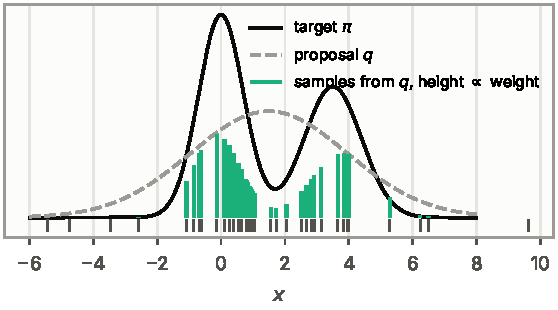
\includegraphics[width=0.75\linewidth]{figures/ch06_importance.pdf}
\caption{Importance sampling. Forty samples are drawn from a wide proposal
$q$ (dashed); each is weighted by $\pi/q$, so that the weighted samples
(green, height proportional to the weight) represent the bimodal target
$\pi$. Samples where $q$ over-represents $\pi$ get small weights.}
\label{fig:importance}
\end{figure}


The self-normalised estimate is
biased for finite $N$
(Exercise~\ref{ex:isbias}), but the bias is $O(1/N)$ and vanishes as $N$
grows (a second-order expansion of the ratio; not proved here, see Doucet
and Johansen in the references).

\section{From the Bayes filter to particles}

The two steps of the Bayes filter translate directly into operations on a
cloud of particles. Suppose the particles $\x_t^{(i)}$, with weights
$w_t^{(i)}$, represent the belief $\bel(\x_t)$.
\begin{itemize}[nosep]
  \item \emph{Predict.} The predicted belief is the distribution of the
    next pose when the current pose is drawn from the belief and one noisy
    step is taken. So take one noisy step from each particle: draw a
    control noise and apply the motion model. The moved particles, with
    the same weights, represent $\belbar(\x_{t+1})$.
  \item \emph{Update.} The new belief is the predicted belief multiplied
    by the likelihood, $\bel\propto p(\z_{t+1}\mid\x)\,\belbar$. This is
    importance sampling with the predicted belief as proposal and the new
    belief as target: the weight of a sample is the ratio of the two,
    which is the likelihood. So multiply the weight of each particle by
    the likelihood of the measurement at that particle, and normalise.
\end{itemize}
\Cref{fig:pfcycle} shows one such cycle on the one-dimensional example of
\cref{fig:bayescycle}, with a third operation, resampling, that is
explained below. The rest of this section makes the argument precise and
states the algorithm.

\begin{figure}[ht]
\centering
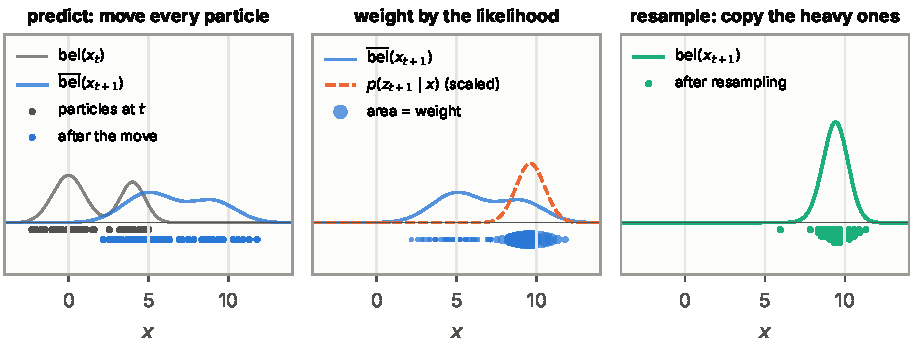
\includegraphics[width=\linewidth]{figures/ch06_pf_cycle.pdf}
\caption{One cycle of a particle filter with $60$ particles, on the example of
\cref{fig:bayescycle}: a two-bump belief, a commanded displacement of $5$
with motion noise, and a measurement whose likelihood peaks at $9.6$. The
curves are the exact
densities computed there: the belief at $t$ (grey), the predicted belief
(blue), the likelihood (dashed) and the new belief (green). Left: each particle (grey dots) is moved by the
commanded displacement plus its own random noise (blue dots). Middle:
each moved particle is weighted by the likelihood of the measurement
(dashed); the area of a dot shows its weight. Right: resampling keeps
$60$ particles of equal weight, by copying the heavy ones (copies are
stacked) and dropping the light ones.}
\label{fig:pfcycle}
\end{figure}

For the precise argument, take the target to be the posterior over the
whole path,
$\pi_t(\x_{0:t})=p(\x_{0:t}\mid\z_{1:t},\uu_{0:t-1})$. It is proportional
to the joint distribution of \cref{prop:joint}, and going from $t$ to
$t+1$ multiplies it by one motion factor and one measurement
factor. So
$\pi_{t+1}(\x_{0:t+1})\propto\pi_t(\x_{0:t})\,p(\x_{t+1}\mid\x_t,\uu_t)\,
p(\z_{t+1}\mid\x_{t+1})$. Choose as proposal ``the previous proposal,
extended by the motion model'':
$q_{t+1}(\x_{0:t+1})=q_t(\x_{0:t})\,p(\x_{t+1}\mid\x_t,\uu_t)$.

\begin{proposition}{Sequential importance sampling with the motion proposal}{sis}
With this proposal, the weights obey
\[
  \tilde w_{t+1}(\x_{0:t+1})\propto\tilde w_t(\x_{0:t})\;
  p(\z_{t+1}\mid\x_{t+1}).
\]
\end{proposition}

\begin{proof}
Formally $\tilde w_{t+1}=\pi_{t+1}/q_{t+1}$, and the factor
$p(\x_{t+1}\mid\x_t,\uu_t)$ appears in both and cancels:
$\tilde w_{t+1}\propto\frac{\pi_t}{q_t}\,p(\z_{t+1}\mid\x_{t+1})$.

This factor is the transition, a distribution without a density
(\cref{prop:degenerate}), so the cancellation is not a division of two
functions and deserves a word. A path is drawn from $q_{t+1}$ by drawing
$\x_{0:t}$ from $q_t$ and then $\x_{t+1}$ from the transition. An average
under $\pi_{t+1}$ is obtained, up to a constant, by drawing $\x_{0:t}$ from
$\pi_t$, then $\x_{t+1}$ from the \emph{same} transition, and weighting by
$p(\z_{t+1}\mid\x_{t+1})$. Replacing the draw from $\pi_t$ by a draw from
$q_t$ weighted by $\tilde w_t$, for every function $g$ of the path,
\[
  \E_{\pi_{t+1}}[g]\;\propto\;\E_{q_{t+1}}\bigl[g\;\tilde w_t(\x_{0:t})\,
  p(\z_{t+1}\mid\x_{t+1})\bigr].
\]
This is the statement
$\mathrm d\pi_{t+1}/\mathrm dq_{t+1}\propto\tilde w_t\,
p(\z_{t+1}\mid\x_{t+1})$ of \cref{def:is}. The transition is sampled,
never evaluated.
\end{proof}

\begin{definition}{Particle filter (sequential importance resampling)}{pf}
Given particles and normalised weights $(\x_t^{(i)},w_t^{(i)})$:
\begin{enumerate}[nosep]
\item \emph{Predict}: draw $\bepsilon^{(i)}\sim\Normal(\vect0,M)$ and set
  $\x_{t+1}^{(i)}=f(\x_t^{(i)},\uu_t+\bepsilon^{(i)})$.
\item \emph{Weight}: $w_{t+1}^{(i)}\propto w_t^{(i)}\,
  p(\z_{t+1}\mid\x_{t+1}^{(i)})$, normalised to sum to one.
\item \emph{Resample} if the effective sample size (\cref{def:ess}) drops
  below a threshold: draw $N$ particles from the cloud with probabilities
  $w^{(i)}$, and reset every weight to $1/N$.
\end{enumerate}
The estimate is the weighted mean (with a circular mean for the heading,
\cref{sec:circular})
and the weighted covariance of the cloud.
\end{definition}

The implementation departs from this definition in two ways, both common
in practice. It propagates the particles with a motion noise inflated by
$1.5$ in standard deviation (covariance $2.25M$, option
\code{motion\_inflation}), which keeps the cloud from becoming too
narrow; and it gives the likelihood $0$ to a particle more than 5 units
outside the lawn. With the inflation the filter no longer samples the
exact transition, so its cloud is somewhat wider than the true belief.
All the particle-filter results of this book use these settings.

\begin{inwords}
\emph{Simulate} the motion for every particle, \emph{score} each one
against the measurement, \emph{clone} the good ones and \emph{drop} the
bad ones. That is the whole algorithm. The sensor model is the same as for
the Kalman filters: a product of Gaussians in range and wrapped bearing
over the visible landmarks.
\end{inwords}

\paragraph{Log-weights.} With four precise landmarks, a particle 50 units
from the truth has a likelihood around $e^{-200}$ relative to a good one:
if its four ranges are each off by about $50=10\,\sigma_r$, each
contributes a factor $e^{-10^2/2}=e^{-50}$. The products underflow
quickly. The implementation adds log-likelihoods and normalises with
$\log\sum_ie^{a_i}=a_{\max}+\log\sum_ie^{a_i-a_{\max}}$ (factor
$e^{a_{\max}}$ out of the sum), in which every exponential is at most
$1$ and the largest is exactly $1$. Fixed rescaling factors, or thresholds on raw
weights, break as soon as the number of visible landmarks or the noise
level changes.

\section{Weight degeneracy}

At each update the weights are multiplied by likelihoods, and after a few
updates they become very uneven: a few particles carry almost all the
weight. One number summarises how uneven they are.

\begin{definition}{Effective sample size}{ess}
For normalised weights, $\ESS=1/\sum_i(w^{(i)})^2\in[1,N]$.
\end{definition}

$\ESS=N$ when all the weights are equal and $\ESS=1$ when one particle
carries all the weight (Exercise~\ref{ex:ess}). It approximates the number
of independent samples drawn directly from the target that would give the
same variance (Kong, Liu and Wong, in the references):
a first-order expansion of the ratio that defines $\hat\varphi_N$ (the
delta method), together with the further approximation that the weights
are uncorrelated with $(\varphi-\E_\pi\varphi)^2$, gives
$\Var(\hat\varphi_N)\approx\Var_\pi(\varphi)\,(1+\mathrm{cv}^2)/N$, where $\mathrm{cv}$ is the coefficient of
variation of the unnormalised weights (their standard deviation divided
by their mean), and $N/(1+\mathrm{cv}^2)$ is
estimated by the ESS.

Run without resampling, sequential importance sampling degenerates
quickly (\cref{fig:ess}). Starting from a Gaussian around the truth with
$N=1000$, the ESS falls below $2$ at step 5: one particle carries all the
weight, the other 999 are wasted computation, and the estimate drifts away
with that single survivor. The variance of the unnormalised weights, with
the measurements treated as random, can only grow over time (Kong, Liu
and Wong, 1994); in a given run it can occasionally decrease. Resampling is what makes the method
work.

\begin{figure}[ht]
\centering
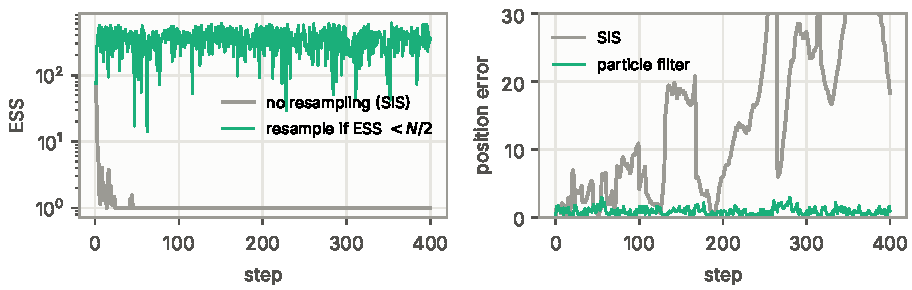
\includegraphics[width=\linewidth]{figures/ch06_ess.pdf}
\caption{Left: ESS before resampling (log scale), $N=1000$. Without
resampling it collapses to 1 within five steps; resampling whenever
$\ESS<N/2$ keeps it in the hundreds. Right: the corresponding position
errors.}
\label{fig:ess}
\end{figure}

\section{Resampling}

Resampling replaces the weighted cloud by an unweighted one that
represents the same belief: it draws $N$ new particles from the old ones,
each old particle being chosen with a probability equal to its weight.
Heavy particles are copied several times, light ones tend to disappear,
and all the new particles get the weight $1/N$ (\cref{fig:pfcycle},
right). The computation is then spent on the particles that matter. The
price is some extra randomness, since the number of copies of each
particle is random, and the way the draw is made decides how much.
\Cref{fig:systematic} shows the method used in this book.

Let $N_i$ be the number of copies of particle $i$ after resampling.
Ideally $N_i$ would be $Nw^{(i)}$, but that is rarely a whole number.

\begin{proposition}{Multinomial and systematic resampling}{resampling}
\emph{Multinomial} resampling draws $N$ indices independently from the
weights.
\emph{Systematic} resampling draws one $U\sim\mathcal U[0,1)$ and selects
the particles whose cumulative-weight intervals contain the $N$ points
$(U+k)/N$, $k=0,\dots,N-1$. Both are unbiased, $\E[N_i]=Nw^{(i)}$, and
\begin{align*}
  \text{multinomial:}&\quad N_i\sim\operatorname{Bin}(N,w^{(i)}),
  &\Var(N_i)&=Nw^{(i)}(1-w^{(i)}),\\
  \text{systematic:}&\quad N_i\in\{\lfloor Nw^{(i)}\rfloor,
  \lceil Nw^{(i)}\rceil\},&\Var(N_i)&=f_i(1-f_i)\le\tfrac14,
\end{align*}
where $f_i=Nw^{(i)}-\lfloor Nw^{(i)}\rfloor$.
\end{proposition}

\begin{proof}
Multinomial: each draw selects $i$ with probability $w^{(i)}$,
independently, so $N_i$ counts the successes of $N$ independent trials of
probability $w^{(i)}$. Systematic: particle $i$ owns an interval $I_i$ of
length $w^{(i)}$ in $[0,1)$, and the points $(U+k)/N$ form a lattice of
spacing $1/N$ with a uniformly random offset. An interval of length
$\ell$ spans $N\ell$ spacings, so it contains at least $\lfloor
N\ell\rfloor$ and at most $\lceil N\ell\rceil$ lattice points. For the
mean: the point $(U+k)/N$ is uniform on $[k/N,(k+1)/N)$, so it falls in
$I_i$ with probability $N\,\abs{I_i\cap[k/N,(k+1)/N)}$; summing over $k$,
$\E[N_i]=N\abs{I_i}=Nw^{(i)}$. A variable
taking the values $m$ and $m+1$ with mean $m+f_i$ takes $m+1$ with
probability $f_i$, hence the variance $f_i(1-f_i)$.
\end{proof}

\begin{figure}[ht]
\centering
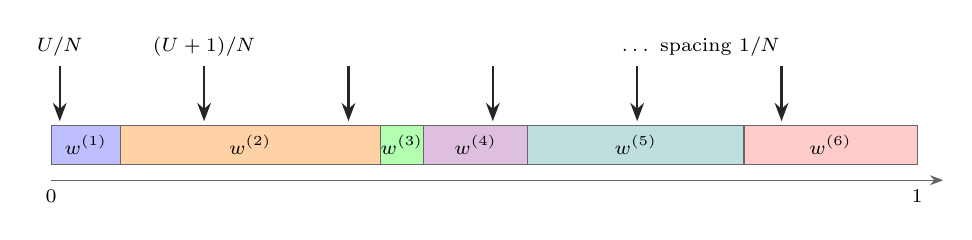
\begin{tikzpicture}[x=11cm,y=1cm,>=Stealth]
  \def\ws{0.08,0.30,0.05,0.12,0.25,0.20}
  \def\cols{{"blue!25","orange!35","green!30","violet!25","teal!25",
    "red!20"}}
  \pgfmathsetmacro{\U}{0.06}
  \foreach \w [count=\i from 0, remember=\c as \cprev (initially 0)] in \ws {
    \pgfmathsetmacro{\c}{\cprev+\w}
    \pgfmathsetmacro{\col}{\cols[\i]}
    \fill[\col] (\cprev,0) rectangle (\c,0.5);
    \draw[black!60] (\cprev,0) rectangle (\c,0.5);
    \pgfmathtruncatemacro{\k}{\i+1}
    \node[font=\scriptsize] at ({(\cprev+\c)/2},0.25) {$w^{(\k)}$};
  }
  \draw[->,black!60] (0,-0.2) -- (1.03,-0.2);
  \node[below,font=\scriptsize] at (0,-0.2) {$0$};
  \node[below,font=\scriptsize] at (1,-0.2) {$1$};
  \foreach \k in {0,...,5} {
    \pgfmathsetmacro{\pos}{(\U+\k)/6}
    \draw[->,thick,black!85] (\pos,1.25) -- (\pos,0.55);
  }
  \pgfmathsetmacro{\pfirst}{\U/6}
  \pgfmathsetmacro{\psecond}{(\U+1)/6}
  \node[above,font=\scriptsize] at (\pfirst,1.25) {$U/N$};
  \node[above,font=\scriptsize] at (\psecond,1.25) {$(U+1)/N$};
  \node[above,font=\scriptsize] at (0.75,1.25) {$\dots$ spacing $1/N$};
\end{tikzpicture}
\caption{Systematic resampling with $N=6$. The weights are laid end to end
on $[0,1)$; one uniform offset $U$ fixes $N$ evenly spaced pointers, and
each particle is copied once per pointer that falls in its interval. Here
particle 2 gets two copies, particles 1, 4, 5 and 6 one each, and particle
3 none: always $\lfloor Nw^{(i)}\rfloor$ or $\lceil Nw^{(i)}\rceil$ (the
expected numbers are $0.48$, $1.8$, $0.3$, $0.72$, $1.5$, $1.2$).}
\label{fig:systematic}
\end{figure}

\begin{figure}[ht]
\centering
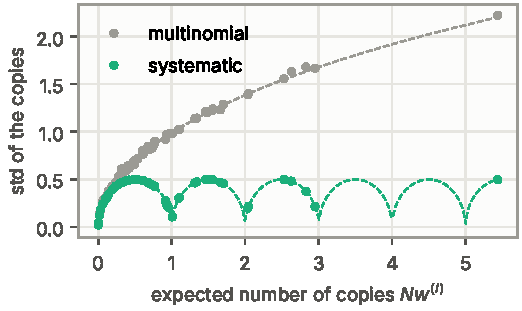
\includegraphics[width=0.62\linewidth]{figures/ch06_resampling.pdf}
\caption{Standard deviation of the number of copies, for 50 particles
and 2\,000 repetitions; dashed lines: the formulas of
\cref{prop:resampling}. Systematic resampling adds almost no noise.}
\label{fig:resampling}
\end{figure}

Each resampling destroys diversity: duplicated particles are identical
until the motion noise separates them. Resampling at every step is
therefore unnecessary and harmful. The filter here resamples only when
$\ESS<N/2$. With four precise landmarks that is still 85\% of the steps,
because each measurement is very informative compared with one step of
motion noise.

On the standard run, with a good initial estimate and identified
landmarks, the particle filter with $N=1000$ has an RMSE of $1.02$,
against $1.01$ for the EKF, at about eight times the cost per step. When
the belief is close to a Gaussian, the particle filter has nothing to add.

\section{Global localisation and sample impoverishment}
\label{sec:global}

A Kalman filter needs an initial guess. A particle filter can start from a
\emph{uniform} belief over the whole lawn and every heading.

\begin{figure}[ht]
\centering
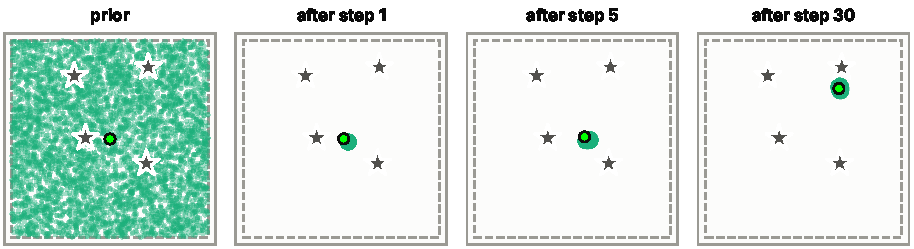
\includegraphics[width=\linewidth]{figures/ch06_global.pdf}
\caption{Global localisation with $N=5000$ (green dot: the robot). One
measurement leaves essentially one compatible particle. After
resampling, all 5\,000 particles are its copies, and the motion noise
slowly spreads them onto the robot.}
\label{fig:global}
\end{figure}

After the first measurement the ESS is $1.0$ out of $5\,000$
(\cref{fig:global}). The reason is a matter of volumes. The prior covers
$320\times320\times2\pi\approx6\times10^5$ units of pose space. After
four ranges and four bearings the posterior has standard deviations of
about $2.6$ and $1.6$ in position and $0.026$\,rad in heading (the
information form of \cref{prop:information}, evaluated at the start
pose; notebook~05 computes them): a box of volume $2.6\times1.6\times0.026\approx0.1$. A uniform
particle falls in that box with probability $0.1/(6\times10^5)\approx
2\times10^{-7}$, so the expected number of particles inside it is about
$2N\times10^{-7}$: far below one for any affordable $N$. The best particle
is a few units from the truth, and the filter must then crawl to it
through the motion noise. This is \emph{sample impoverishment}: the
posterior is much narrower than the spacing between the particles.

\begin{inwords}
Particles are only useful where the probability is, and when the
likelihood is sharp, ``where the probability is'' is a tiny region that a
uniform cloud almost never hits. More particles help only slowly; in
higher dimensions the volume ratio explodes, which is the particle
filter's real weakness.
\end{inwords}

The remedies all widen the effective likelihood or move particles
towards it: \emph{roughening} (a small jitter after resampling), a
\emph{tempered} likelihood $p(\z\mid\x)^\beta$ with $\beta<1$ for the
first updates, or \emph{sensor resetting}, which draws some particles
directly from the poses compatible with the measurement.

\section{Unknown data association and multimodal beliefs}
\label{sec:pf-association}

When the sensor does not say which landmark it saw, the likelihood of one
measurement is a mixture over the landmarks that could have produced it:
\[
  p(\z_k\mid\x)=\frac1{n_\ell}\sum_{j=1}^{n_\ell}\Normal\bigl(\z_k;\,
  h_j(\x),\,R_1\bigr),
\]
assuming each landmark equally likely a priori. A particle filter simply
evaluates it: every particle is scored against every possible
association, and no decision is ever taken. Attributing each measurement
to the nearest landmark, as an EKF must, amounts to replacing the sum by
its largest term.

Take a different world for this experiment: four landmarks on a square,
at $(\pm80,\pm80)$. The lawn is then symmetric under rotations by
$90^\circ$ and, without identities, four poses explain the
measurements equally well forever. The true posterior has four bumps of
mass $1/4$ each. \Cref{fig:modes} shows what the particle filter does with
it (the noise is raised to $\sigma_r=15$ and $\sigma_\phi=0.25$, so that
$20\,000$ particles resolve all four modes from a uniform start).

\begin{figure}[ht]
\centering
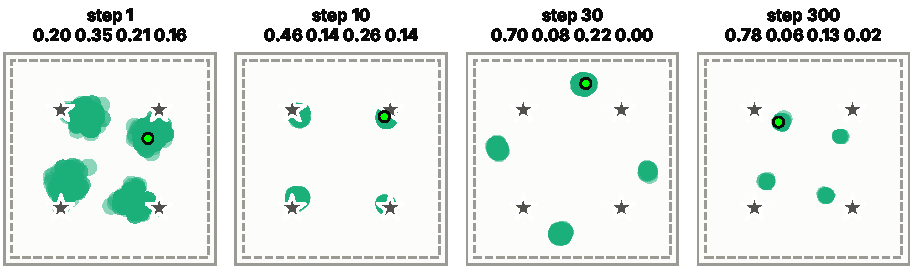
\includegraphics[width=\linewidth]{figures/ch06_modes.pdf}
\caption{Symmetric landmarks, unknown identities, $N=20\,000$. Above each
panel: the mass of the four modes (rotations of the true pose). The
correct posterior has four masses of $0.25$ forever; the particle
estimates drift.}
\label{fig:modes}
\end{figure}

The cloud correctly splits into four clusters. But the masses
($0.20$, $0.35$, $0.21$, $0.16$ after one step) drift: after 30 steps one
mode holds $0.70$ and another $0.005$ (notebook~05 prints them), fewer than a hundred particles. A
mode that loses its last particle never comes back. With fewer particles
it happens much sooner: with $N=2000$ only one mode is left by step 30 in
each of three runs.

The drift has a simple explanation, which needs one notion. A
\emph{martingale} is a random process whose expected next value, given its
present value, is the present value: it has no tendency to go up or down,
but it does fluctuate.

\begin{proposition}{Mode masses are martingales with absorbing ends}{wrightfisher}
Idealise the situation: two modes $A$ and $B$ whose particles all have
the same likelihood, so that the weights stay equal, and multinomial
resampling at every step. Let
$m_t$ be the fraction of particles in $A$. Then $(m_t)$ is a martingale,
$\E[m_{t+1}\mid m_t]=m_t$ and $\Var(m_{t+1}\mid m_t)=m_t(1-m_t)/N$. It
reaches $0$ or $1$ in finite time with probability one, and reaches $1$
with probability $m_0$.
\end{proposition}

\begin{proof}
After resampling, the number of particles in $A$ is
$\operatorname{Bin}(N,m_t)$ (each draw lands in $A$ with probability
$m_t$), so $Nm_{t+1}$ has mean $Nm_t$ and variance $Nm_t(1-m_t)$;
dividing by $N$ and $N^2$ gives the mean and variance of $m_{t+1}$.

\emph{Absorption.} The states $0$ and $1$ are absorbing: an empty mode
receives no draws, and a full one receives all of them. From any other
state $m$, all $N$ draws miss $A$ with probability $(1-m)^N>0$; over the
finitely many states $k/N$, $0<k<N$, this probability is at least some
$c>0$. So the probability of not being absorbed during $k$ steps is at
most $(1-c)^k\to0$: absorption happens with probability one, at a random
time $\tau$.

\emph{Where it ends.} Taking expectations in $\E[m_{t+1}\mid m_t]=m_t$
gives $\E[m_{t+1}]=\E[m_t]$, so $\E[m_t]=m_0$ for every $t$. After $\tau$
the fraction no longer changes, so $m_t\to m_\tau$ with probability one;
$0\le m_t\le1$, so dominated convergence gives $\E[m_\tau]=m_0$. Since
$m_\tau\in\{0,1\}$, $\E[m_\tau]=\Pr(m_\tau=1)$, which is therefore $m_0$.
\end{proof}

\begin{inwords}
This is the neutral Wright--Fisher model of population genetics: genetic
drift. Without any evidence favouring one mode, the particle population
still ``chooses'' one at random, and the filter ends up claiming a
certainty that the data do not support. The proposition isolates the
noise of resampling. In \cref{fig:modes} the weighting step adds a
larger Monte Carlo noise of its own: with random weights, the variance
per step gains a term from the spread of the weight of each mode, and the
drift is much faster than the resampling noise alone would give
(Exercise~\ref{ex:fixation} predicts about $1\,400$ resamplings to halve
the spread of a $50/50$ split with $N=2000$, against one mode left by step
30 in the runs above). Systematic resampling reduces the resampling noise,
but not the weighting noise, so the drift remains. More particles slow it down
(the variance per step is $\propto1/N$); nothing stops it. The weighted
mean is meaningless here; a multimodal belief should be reported by its
modes.
\end{inwords}

\section{The kidnapped robot}
\label{sec:amcl}

\emph{Kidnapped} is the standard name in robotics (the \emph{kidnapped
robot problem}) for a robot that is picked up and moved somewhere else
without being told: someone lifts the robot and puts it down on another
part of the lawn. The filter keeps receiving ordinary commands and
measurements, and nothing tells it that the robot has moved. This is
harder than global localisation: there the filter \emph{knows} that it does
not know where the robot is; here it is \emph{confidently wrong}, and must
first discover that its belief is wrong. A converged particle filter has
no particles near the new pose, so it can only crawl there through the
motion noise, if at all.

The way to discover it is \cref{prop:evidence}: the normaliser of the
Bayes filter is the predictive likelihood of the measurement, and a
kidnapping makes it collapse.

\begin{proposition}{Estimating the predictive likelihood}{avglik}
Let $(\x^{(i)},w^{(i)})$ be the predicted cloud, approximating
$\belbar(\x_{t+1})$. Then
\[
  \hat\ell_{t+1}=\sum_iw^{(i)}\,p(\z_{t+1}\mid\x^{(i)})
  \longrightarrow\int p(\z_{t+1}\mid\x)\,\belbar(\x)\,\mathrm d\x=
  \eta_{t+1}^{-1}
\]
as $N\to\infty$, assuming that the predicted cloud is a consistent
approximation of $\belbar$.
\end{proposition}

\begin{proof}
For independent draws from a fixed proposal this is
\cref{prop:isconsistent} with $\varphi(\x)=p(\z_{t+1}\mid\x)$, which is
bounded, and the target $\belbar$; the identification of the limit is
\cref{prop:evidence}. A resampled and propagated cloud is not a set of
independent draws, and its consistency is a theorem of its own, not proved
here (see Doucet and Johansen in the references).
\end{proof}

The idea of \emph{augmented} Monte Carlo localisation is to watch this
number over time. While the filter is tracking, the measurements are
explained about as well as usual. After a kidnapping they are suddenly
explained much worse than usual. ``Usual'' is measured by a long-term
average of $\hat\ell_t$, and ``now'' by a short-term one. Both are
\emph{exponential averages}: at each step the average moves a fraction
$\alpha$ of the way towards the new value, so that a small $\alpha$ gives
a long memory and a large $\alpha$ a short one.

\begin{definition}{Augmented MCL}{amcl}
Maintain two exponential averages of $\hat\ell_t$, a slow one and a fast
one ($0<\alpha_{\mathrm{slow}}\ll\alpha_{\mathrm{fast}}<1$):
\[
  w_{\mathrm{slow}}\leftarrow w_{\mathrm{slow}}+\alpha_{\mathrm{slow}}
  (\hat\ell_t-w_{\mathrm{slow}}),\qquad
  w_{\mathrm{fast}}\leftarrow w_{\mathrm{fast}}+\alpha_{\mathrm{fast}}
  (\hat\ell_t-w_{\mathrm{fast}}),
\]
and, whenever $p=\max(0,1-w_{\mathrm{fast}}/w_{\mathrm{slow}})$ is
positive, resample and replace each particle, with probability $p$, by a
pose drawn uniformly over the lawn.
\end{definition}

When the measurements suddenly become hard to explain, the fast average
drops below the slow one, and a fraction of the particles is scattered
over the lawn; some land near the new pose and are quickly amplified by
the next updates. While tracking normally, $w_{\mathrm{fast}}$ stays
above $w_{\mathrm{slow}}$ and nothing is injected. (In \cref{fig:amcl} it
is about six times above, because both start from the first value of
$\hat\ell$, after the global start, and $w_{\mathrm{slow}}$ still
remembers those low values.) \Cref{fig:amcl} shows the mechanism on one
kidnapping.

\begin{figure}[ht]
\centering
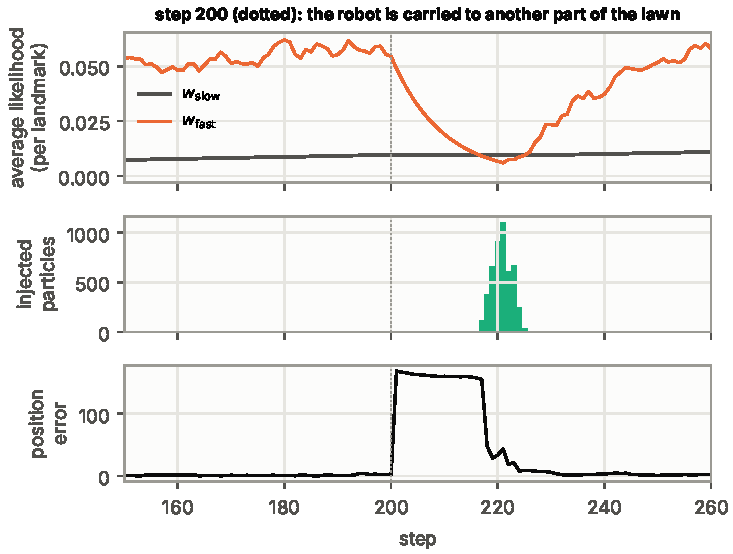
\includegraphics[width=0.8\linewidth]{figures/ch06_amcl.pdf}
\caption{Augmented MCL around the kidnapping of \cref{fig:kidnap}: at step $200$
(dotted) the robot is carried to another part of the lawn (unknown
landmark identities, $N=3000$). Top: after the kidnapping the measurement likelihood is
close to zero, so the fast average decays by the factor
$1-\alpha_{\mathrm{fast}}=0.9$ per step; the slow one barely moves. Middle: once
$w_{\mathrm{fast}}<w_{\mathrm{slow}}$ (step 217), random particles are
injected. Bottom: some of them land near the new pose, and the position
error drops back to a few units.}
\label{fig:amcl}
\end{figure}

The implementation averages the \emph{per-landmark} likelihood (the
geometric mean over the visible landmarks, $\hat\ell_t^{1/m}$), so that
the scale of $\hat\ell$ does not jump when the number of visible landmarks
changes.

\begin{figure}[ht]
\centering
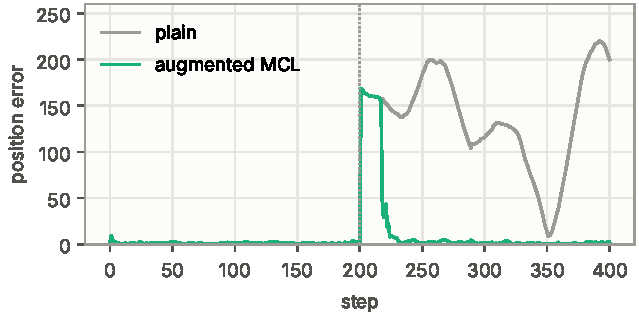
\includegraphics[width=0.75\linewidth]{figures/ch06_kidnap.pdf}
\caption{Kidnapped at step 200 (dotted line), unknown landmark identities,
$N=3000$, seed 7. Without injection the filter does not find the robot
again: its error dips briefly around step 350 and grows back. With
augmented MCL it recovers within about 25 steps and stays locked.}
\label{fig:kidnap}
\end{figure}

Over eight kidnappings (unknown identities, $N=3000$), the number of steps
until the error stays below 10 is $20$ to $41$ with augmented MCL.
Without it, four of the eight runs never recovered within 200 steps, and
the other four took $51$ to $113$ steps (the run of \cref{fig:kidnap} is
one of the eight). All the kidnapping runs use a roughening of $0.5$
(below).

\begin{practice}[\nb{05\_particle\_filter.ipynb}, \code{pf.py}]
\code{ParticleFilter} stores the particles as an $(N,3)$ array and the
log-weights as an $N$-vector. Options: \code{init="global"} or a Gaussian;
\code{association="known"} or \code{"unknown"} (the mixture likelihood);
\code{resample\_threshold} (on $\ESS/N$); \code{systematic\_resample} or
\code{multinomial\_resample}; \code{roughening}; and
\code{recovery=(alpha\_slow, alpha\_fast)} for augmented MCL. The filter
records its ESS, resampling and injection history. The notebook reproduces
\cref{fig:ess,fig:resampling,fig:global,fig:modes,fig:kidnap} and counts
the surviving modes for several $N$; the other figures are produced by
\code{book/figures/make\_figures.py}.
\end{practice}

\begin{mower}
Robot mowers are kidnapped all the time: carried to another part of the
garden, lifted by a curious child, or simply switched off in the shed and
on again on the lawn. Most have a lift sensor, which tells the filter that
a kidnapping happened and lets it re-initialise globally. Augmented MCL
covers the cases a lift sensor misses, such as wheels sliding on a wet
slope.
\end{mower}

\section*{What to remember from this chapter}
\addcontentsline{toc}{section}{What to remember}

\begin{enumerate}[nosep]
  \item A particle filter represents the belief by weighted samples. One
    cycle: move every particle with the noisy motion model, multiply its
    weight by the likelihood of the measurement, and resample when the
    weights become too uneven.
  \item It is importance sampling applied step by step, with the motion
    model as proposal; the motion model is only sampled, never evaluated.
  \item Without resampling the weights degenerate: one particle ends up
    with all the weight. The effective sample size measures this, and
    systematic resampling is the low-noise way to resample.
  \item The filter can start from a uniform belief and handle unknown
    landmark identities and several hypotheses, which the Kalman filters
    cannot.
  \item Its weaknesses are sample impoverishment (a sharp likelihood that
    no particle hits), the random loss of modes, and a cost that grows
    quickly with the dimension of the state.
  \item A kidnapped robot is detected by the collapse of the measurement
    likelihood; augmented MCL then injects random particles.
\end{enumerate}

\FloatBarrier
\section*{Exercises}
\addcontentsline{toc}{section}{Exercises}

\begin{enumerate}[label=\textbf{6.\arabic*},ref=6.\arabic*]
\item\label{ex:ess} Show that $1\le\ESS\le N$, with equality on the right
  if and only if all weights are equal and on the left if and only if one
  weight is $1$. Show that $\ESS=N/(1+N^2s^2)$, where $s^2$ is the
  empirical variance of the normalised weights.
\item\label{ex:isbias} Let the target be $\pi=\Normal(1,1)$, the proposal
  $q=\Normal(0,1)$ and $\varphi(x)=x$. For $N=1$, what does the
  self-normalised estimate return, and what is its mean? Conclude that it
  is biased.
\item\label{ex:stratified} \emph{Stratified} resampling draws one
  independent uniform in each $[k/N,(k+1)/N)$ instead of one shared
  offset. Show that it is unbiased and that $\Var(N_i)\le Nw^{(i)}
  (1-w^{(i)})$ for every $i$.
\item\label{ex:fixation} In \cref{prop:wrightfisher}, show that
  $\E[m_{t}(1-m_{t})]=m_0(1-m_0)(1-1/N)^t$. After how many resamplings
  has the ``heterozygosity'' of a $50/50$ split dropped by half, for
  $N=2000$?
\end{enumerate}

\subsection*{Solutions}

\solution{6.1} With $\sum_iw_i=1$ and $w_i\ge0$, $\sum_iw_i^2\le
\sum_iw_i\max_kw_k\le1$, with equality iff one weight is $1$. By
Cauchy--Schwarz, $1=(\sum_iw_i)^2\le N\sum_iw_i^2$, with equality iff all
the weights are equal. The empirical mean of the weights is $1/N$, so
$s^2=\frac1N\sum_iw_i^2-\frac1{N^2}$, i.e.\ $\sum_iw_i^2=Ns^2+1/N$ and
$\ESS=1/(Ns^2+1/N)=N/(1+N^2s^2)$.

\solution{6.2} With one sample the normalised weight is $1$, so
$\hat\varphi_1=X^{(1)}$, whose mean under $q$ is $0$, not $\E_\pi[X]=1$.
The ratio of two unbiased estimates is not unbiased; the bias of the
self-normalised estimate shrinks like $1/N$.

\solution{6.3} The pointer $U_k\sim\mathcal U[k/N,(k+1)/N)$ falls in
particle $i$'s interval $I_i$ with probability $N|I_i\cap[k/N,
(k+1)/N)|=:p_{ik}$, so $\E[N_i]=\sum_kp_{ik}=N|I_i|=Nw^{(i)}$. The
pointers are independent, so $N_i$ is a sum of independent Bernoulli
variables with parameters $p_{ik}$ and
$\Var(N_i)=\sum_kp_{ik}(1-p_{ik})$. For a fixed sum $\sum_kp_{ik}=
Nw^{(i)}$, $\sum_kp_{ik}^2\ge(\sum_kp_{ik})^2/N=Nw^{(i)2}$ by
Cauchy--Schwarz, so $\Var(N_i)\le Nw^{(i)}-Nw^{(i)2}$.

\solution{6.4} Let $h_t=m_t(1-m_t)$. Given $m_t$,
$\E[m_{t+1}^2]=\E[m_{t+1}]^2+\Var(m_{t+1})=m_t^2+m_t(1-m_t)/N$, so
\[
  \E[h_{t+1}\mid m_t]=\E[m_{t+1}]-\E[m_{t+1}^2]
  =m_t-m_t^2-\frac{m_t(1-m_t)}N=h_t\Bigl(1-\frac1N\Bigr).
\]
Taking expectations, $\E[h_{t+1}]=(1-1/N)\,\E[h_t]$, and after $t$ steps
$\E[h_t]=(1-1/N)^th_0$. For $N=2000$,
$(1-1/N)^t=1/2$ gives $t=\log2/(-\log(1-1/2000))\approx1386$
resamplings: slow, but certain, and faster with fewer particles or
noisier weights.

\chapter{Choosing a filter}
\label{ch:choosing}

All the filters of this book have now run on the same robot and the same
data. This chapter collects the results of the showdown notebook, draws
the practical conclusions, and closes with the bridge from filtering to
the smoothing view used by modern localisation and mapping systems.

\section{The showdown}

Each scenario is repeated over several random seeds. A filter is
\emph{lost} when its median position error over the last 50 steps exceeds
10 units. The EKF, UKF and particle filter use the range--bearing sensor;
the KF uses the compass and the GPS (Chapter~\ref{ch:kalman}), so its
numbers measure a different sensor suite. The figures below are averages
over several runs, each started from an initial estimate drawn at random
around the truth. They therefore differ slightly from those quoted in the
previous chapters, which were for the single standard run started from
the exact pose (for the EKF, $1.16$ here against $1.01$ there).

\paragraph{Tracking.} A good initial estimate, drawn from
$\Normal(\x_0,P_0)$, four landmarks always visible and identified, 10
runs:
\begin{center}
\begin{tabular}{@{}lrrrr@{}}
\toprule
& RMSE & mean NEES & ms/step & lost\\
\midrule
KF (compass + GPS) & 2.01 & 1.81 ($n=2$) & 0.04 & 0/10\\
EKF & 1.16 & 3.03 & 0.11 & 0/10\\
UKF & 1.16 & 2.92 & 0.16 & 0/10\\
PF ($N=1000$) & 1.22 & 2.68 & 0.75 & 0/10\\
\bottomrule
\end{tabular}
\end{center}
The three landmark filters are equally accurate and all consistent. The
EKF is the cheapest. This is the common case, and the EKF is the right
tool for it.

\paragraph{Uncertain start.} $\sigma_{xy}=30$, $\sigma_\theta=0.8$, sensor
range 110, 10 runs; the particle filter starts from the uniform prior
over the lawn and needs no guess at all:
\begin{center}
\begin{tabular}{@{}lrrr@{}}
\toprule
& RMSE & mean NEES (after step 20) & lost\\
\midrule
EKF & 1.83 & 3.0 & 0/10\\
UKF & 1.83 & 2.9 & 0/10\\
PF ($N=5000$, uniform prior) & 2.13 & 11.3 & 0/10\\
\bottomrule
\end{tabular}
\end{center}
Everybody converges. The EKF's over-confident transient
(\cref{fig:ekftransient}) is over by step 20. The particle filter, starting
from nothing, takes longer to settle, and its NEES of $11.3$ (against $3$)
is the price of sample impoverishment: after the first update collapsed
the cloud (\cref{fig:global}), the particles are too few and too alike,
and the cloud claims more precision than it has.

\paragraph{Kidnapped, landmarks identified.} At step 200 the robot is
moved to $(100,-100)$ and turned to face west; 8 runs. Steps until the
error stays below 10:
\begin{center}
\begin{tabular}{@{}lrl@{}}
\toprule
& median & all runs\\
\midrule
EKF & 66 & 88, 43, 48, 60, 75, 83, 33, 71\\
UKF & 66 & identical to the EKF\\
PF (augmented MCL) & 21 & 18, 76, 20, 18, 22, 26, 25, 14\\
\bottomrule
\end{tabular}
\end{center}
A surprise: the Kalman filters \emph{do} recover, every time, but slowly.
With every landmark identified, each measurement is close to a full
position fix, and the likelihood has a single peak. Even a wildly wrong
Gaussian is pulled towards it, step after step. The pull is slow because
the covariance is small (the filter was confident before the kidnapping),
so the filter keeps trusting its prediction and moves only a little at
each update. The particle filter injects random particles over the lawn
(\cref{sec:amcl}) and reaches the new pose in about twenty steps, three times sooner. The real lesson is that \emph{identified landmarks
make the problem unimodal}, the situation in which a Gaussian filter is
at home.

\paragraph{Unknown data association.} The EKF uses nearest-neighbour
association (\cref{sec:ekf-association}); the particle filter, the
mixture likelihood with augmented MCL (\cref{sec:pf-association,sec:amcl});
8 runs per case:
\begin{center}
\begin{tabular}{@{}lcc@{}}
\toprule
& EKF (nearest neighbour) & PF (mixture + recovery)\\
\midrule
uncertain start ($\sigma_{xy}=80$, any heading) & lost 4/8 & lost 0/8\\
kidnapped & lost 3/8 & lost 0/8\\
\bottomrule
\end{tabular}
\end{center}
Without identities the EKF is fragile. Once its estimate is off by more
than about half the spacing of the landmarks, it associates measurements
with the wrong landmarks, each wrong update pulls it further away and
shrinks its covariance, and it often does not come back. The particle filter
never commits to an association and, with random injection, finds the
robot again after a kidnapping.

\section{Scorecard}

\begin{center}
\small
\begin{tabular}{@{}p{3.3cm}p{2.2cm}p{2.6cm}p{2.6cm}p{2.9cm}@{}}
\toprule
& KF & EKF & UKF & PF\\
\midrule
needs & linear models & Jacobians & model evaluations &
  a likelihood to evaluate\\
tracking & good & good, cheapest & good & good, $7$ to $8\times$ the cost\\
uncertain start & --- & converges, over-confident at first &
  converges, consistent & no guess needed; slower, over-confident cloud\\
kidnapped, identified landmarks & --- & recovers slowly & recovers
  slowly & recovers fast (injection)\\
unknown association & --- & often lost & (same problem) & recovers\\
multimodal belief & no & no & no & yes, but modes can die\\
cost per step & $O(n^3)$ & $O(n^3)$ & $O(n^3)$, $2n+1$ points &
  $O(N)$, $N$ grows fast with $n$\\
\bottomrule
\end{tabular}
\end{center}

\begin{inwords}
Use the EKF when the belief is roughly Gaussian and the models are smooth;
check its Jacobians by finite differences. Use the UKF when the
uncertainty is large compared with the curvature of the models, or when
the Jacobians are painful. Use the particle filter when the belief can be
multimodal (global localisation, ambiguous or unidentified landmarks,
kidnapping) and the state is low-dimensional. Whatever the filter,
test its consistency (NEES in simulation, NIS on real data), not only its
accuracy.
\end{inwords}

\section{Closing the loop}
\label{sec:closedloop}

In every experiment so far the filter replayed a \emph{recorded run}. The
commands had been chosen beforehand by the pilot of the simulation, and
the filter only had to find out where the robot was. This is how filters
are compared, since all of them see the same data, and it is how one works
with the log of a real robot.

On a robot at work the filter is \emph{in the loop}. At each step a
controller looks at the filter's current estimate $\hx_t$ and chooses the
command, the robot moves, its sensors read, and the filter is updated:
\[
  \uu_t=\pi(\hx_t),\qquad
  \x_{t+1}=f(\x_t,\uu_t+\bepsilon_t),\qquad
  \z_{t+1}=h(\x_{t+1})+\vv_{t+1},\qquad
  \hx_{t+1}\ \text{from}\ (\hx_t,\uu_t,\z_{t+1}).
\]
The controller $\pi$ never sees the true pose $\x_t$. It can only correct
the error it sees, the distance between the \emph{estimate} and the
planned path. What matters for the task is the distance between the
\emph{true} position and the planned path, called the \emph{cross-track
error}. The two agree only as far as the estimate is good.

The experiment uses the task of a robot lawnmower: drive along parallel
stripes, 40 units apart, back and forth across the lawn (a path of 2060
units, about 500 steps). The controller is a simple path follower: it aims
at the point of the path 12 units ahead of the estimated position, with a
turn limited to $0.5$\,rad per step.

\begin{figure}[ht]
\centering
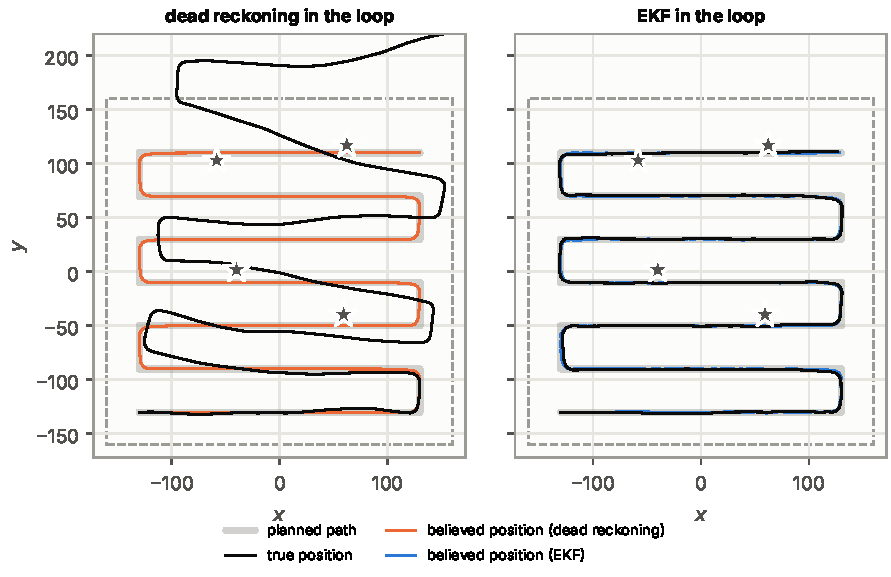
\includegraphics[width=\linewidth]{figures/ch07_closed_loop.pdf}
\caption{The filter in the loop, on a mowing pattern (seed 1). Grey: the
planned stripes. Colour: where the robot believes it is. Black: where it
really is. Left: with dead reckoning the believed path lies exactly on
the plan, while the true robot drifts and leaves the lawn. Right: with the
EKF the estimate follows the truth, so correcting the estimate corrects
the robot.}
\label{fig:closedloop}
\end{figure}

\Cref{fig:closedloop} shows the two extremes. With \emph{dead reckoning}
in the loop (the commands are integrated and no sensor is read), the
estimate is by construction where the controller wants it: the robot
believes that it follows the stripes perfectly, and nothing tells it that
it does not. With a filter in the loop, an error of the true position
shows up in the measurements, then in the estimate, and the controller
removes it. Over 10 runs:
\begin{center}
\begin{tabular}{@{}lrrr@{}}
\toprule
filter in the loop & cross-track RMS & estimation RMSE & left the lawn\\
\midrule
dead reckoning & 27.3 & 90.5 & 10/10\\
KF (compass + GPS) & 1.24 & 2.11 & 0/10\\
EKF & 0.83 & 1.18 & 0/10\\
UKF & 0.82 & 1.18 & 0/10\\
PF ($N=1000$) & 0.85 & 1.27 & 0/10\\
\bottomrule
\end{tabular}
\end{center}
Every filter keeps the robot on its stripes to within about one unit. The
estimation errors are close to those of the tracking scenario above (for
the EKF, $1.18$ against $1.16$): being in the loop does not make the filter's task
harder here. The cross-track error is smaller than the estimation error
because it counts only the part of the error that lies across the path.

Two remarks. First, in the loop the command is computed from the filter's
own estimate, hence from the measurements that the filter has received.
This is the case in which the recursion of \cref{thm:bayes} is exact,
although the controls are not fixed in advance (\cref{sec:bayesnet-mower},
complement). Second, the loop also carries the filter's failures to the
wheels: a filter that is lost, after a kidnapping or a wrong association,
steers the robot with the same confidence as before. This is the practical
reason to monitor consistency (NIS) on a real robot, and to stop when the
estimate is no longer credible.

\begin{practice}[\nb{07\_closing\_the\_loop.ipynb}, \code{control.py}]
\code{stripes\_path} builds the waypoints, \code{PathFollower} is the
controller, and \code{simulate\_closed\_loop} runs any filter of the
package in the loop and returns the run that it produced together with the
filter's estimates. \code{DeadReckoning} is the filter that never reads a
sensor. The notebook reproduces \cref{fig:closedloop} and the table, and
suggests experiments: a limited sensor range, a wrong initial pose, a
kidnapping.
\end{practice}

\section{From filtering to smoothing}
\label{sec:smoothing}

All the filters of this book estimate the \emph{current} state and then
forget the past. Yet a later measurement still carries information about
an earlier pose (\cref{sec:bayesnet-mower}, statement~(d)). Estimating the
whole trajectory from all the measurements is called \emph{smoothing}. For
the current pose of a linear-Gaussian model the two give the same answer,
so filtering loses nothing there.

As in \cref{prop:gaussnewton}, $\norm{\vect e}_A^2=\vect e\T A^{-1}\vect e$
is the squared Mahalanobis norm: the squared size of $\vect e$ counted in
standard deviations of a noise of covariance $A$.

\begin{proposition}{The Kalman filter solves a least-squares problem}{batch}
For the linear-Gaussian model of \cref{def:lgmodel}, the trajectory
$\x^\star_{0:T}$ that minimises
\[
  J(\x_{0:T})=\tfrac12\norm{\x_0-\hx_0}_{P_0}^2+\tfrac12\sum_{t=0}^{T-1}
  \norm{\x_{t+1}-F_t\x_t-B_t\uu_t}_{Q_t}^2+\tfrac12\sum_{t=1}^T
  \norm{\z_t-H_t\x_t}_{R_t}^2
\]
has $\x^\star_T=\hx_T$, the Kalman filter's estimate at time $T$.
\end{proposition}

\begin{proof}
By \cref{prop:joint}, $-\log p(\x_{0:T}\mid\z_{1:T},\uu)=J(\x_{0:T})
+\text{const}$, and $J$ is a positive definite quadratic, so the posterior
over the whole trajectory is Gaussian and its mode $\x^\star_{0:T}$ is its
mean. The mean of a marginal is the marginal of the mean, so
$\x^\star_T=\E[\x_T\mid\z_{1:T},\uu]$, which is the mean of
$\bel(\x_T)$: $\hx_T$ by \cref{thm:kf}.
\end{proof}

\begin{figure}[ht]
\centering
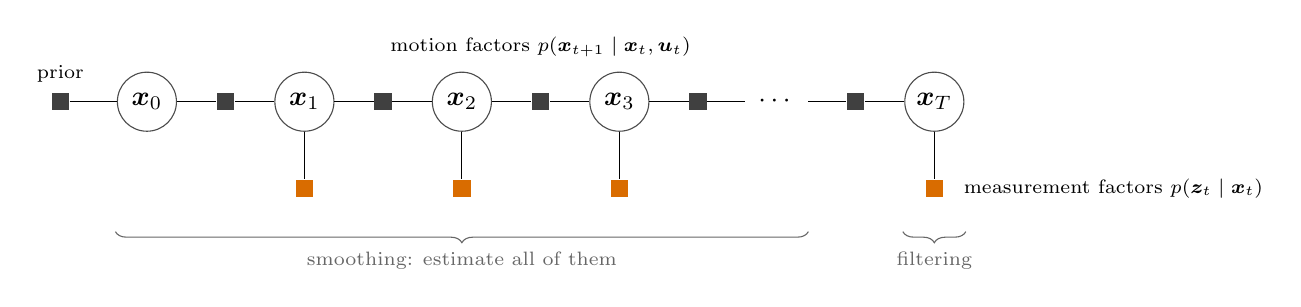
\begin{tikzpicture}[>=Stealth,
    var/.style={circle,draw=black!70,fill=white,minimum size=7.5mm,
      inner sep=0pt},
    fac/.style={rectangle,fill=black!75,minimum size=2.2mm,inner sep=0pt},
    meas/.style={rectangle,fill=orange!85!black,minimum size=2.2mm,
      inner sep=0pt}]
  \foreach \i/\lab in {0/0,1/1,2/2,3/3,5/T}{
    \node[var] (x\i) at (2*\i,0) {$\x_{\lab}$};}
  \node at (8,0) {$\cdots$};
  \node[fac,label={[font=\scriptsize]above:prior}] (p0) at (-1.1,0) {};
  \draw (p0) -- (x0);
  \foreach \a/\b in {0/1,1/2,2/3}{
    \node[fac] (m\a) at (2*\a+1,0) {};
    \draw (x\a) -- (m\a) -- (x\b);}
  \node[fac] (m3) at (7,0) {}; \draw (x3) -- (m3) -- (7.6,0);
  \node[fac] (m4) at (9,0) {}; \draw (8.4,0) -- (m4) -- (x5);
  \foreach \i in {1,2,3,5}{
    \node[meas] (z\i) at (2*\i,-1.1) {};
    \draw (x\i) -- (z\i);}
  \node[font=\scriptsize,right] at (10.25,-1.1) {measurement factors
    $p(\z_t\mid\x_t)$};
  \node[font=\scriptsize,above] at (5,0.45) {motion factors
    $p(\x_{t+1}\mid\x_t,\uu_t)$};
  \draw[decorate,decoration={brace,amplitude=4pt,mirror},black!60]
    (-0.4,-1.65) -- (8.4,-1.65) node[midway,below=4pt,font=\scriptsize]
    {smoothing: estimate all of them};
  \draw[decorate,decoration={brace,amplitude=4pt,mirror},black!60]
    (9.6,-1.65) -- (10.4,-1.65) node[midway,below=4pt,font=\scriptsize]
    {filtering};
\end{tikzpicture}
\caption{The factor graph of \cref{prop:joint}: one variable per pose
(circles) and one factor per term of the cost $J$ (squares): a prior,
the motion between consecutive poses, and the measurement at each pose.
A filter estimates only the newest pose and summarises the rest by its
belief; a smoother estimates the whole chain, and can still correct the
past.}
\label{fig:factorgraph}
\end{figure}

\Cref{fig:factorgraph} draws the structure of $J$. It is the Bayesian
network of \cref{fig:bayesnet} seen from the side of the cost: each
conditional distribution of the network becomes one factor, that is, one
squared term of $J$.

The cost $J$ divides by $Q_t$, which must therefore be invertible. For
the robot's motion model it is not: $Q_t=VMV\T$ has rank $2$
(\cref{prop:firstorder}). The motion term is then written with the
control noise as the unknown, $\tfrac12\norm{\bepsilon_t}_M^2$ subject to
$\x_{t+1}=f(\x_t,\uu_t+\bepsilon_t)$, which is the case announced at the
end of \cref{sec:shape}.

In the non-linear case
the equivalence between filtering and smoothing breaks. The EKF linearises
each
measurement once, at the estimate available \emph{at that time}, and
never revisits that decision, even after later measurements have shown the
estimate to be wrong. The minimiser of the same cost $J$ with $f$ and $h$
non-linear can instead be found by Gauss--Newton over the whole
trajectory, re-linearising \emph{every} past state at each iteration;
\cref{prop:gaussnewton} is the one-state, one-iteration special case. This
is \emph{smoothing}, and it is the basis of modern localisation and
mapping (SLAM): the cost is a sum of small terms, each involving a few
variables (\cref{prop:joint}), so its Hessian is sparse, and the problem
can be drawn as a \emph{factor graph} and solved efficiently even with
thousands of poses. Filtering remains the right tool when only the current
state matters and the models are nearly linear over the uncertainty, or
when the belief is multimodal and a particle filter is needed; smoothing
when the past can still be corrected and the cost of keeping it is
affordable.

The companion course \url{https://github.com/CL-BZH/vslam-course} takes
up exactly this point of view, with the same robot lawnmower as its running
example: the SLAM problem as nonlinear least squares over a factor graph,
rigid motion and Lie groups, cameras, bundle adjustment, loop closure, and
fusion with an IMU, wheel odometry and RTK-GNSS.

\begin{practice}[\nb{06\_showdown.ipynb}]
The notebook runs the four scenarios above with every filter, prints the
tables of this chapter and plots the error curves of the kidnapping and
unknown-association runs. \code{run\_filter} drives any filter of the
package over a \code{Run} and records its means, covariances and timing,
so a new filter only needs \code{predict}, \code{update}, \code{mean} and
\code{cov} to join the comparison.
\end{practice}

\begin{mower}
A practical mower uses several of these filters at once. An EKF (or UKF)
fuses wheel odometry, an IMU and RTK-GNSS for smooth, cheap tracking;
its NIS is monitored, and when it fails, or when a lift sensor reports a
kidnapping, a particle filter re-localises the mower against a map before
handing a Gaussian back to the EKF. Mapping the garden in the first
place, or localising with a camera, is a smoothing problem.
\end{mower}

\FloatBarrier
\section*{Exercises}
\addcontentsline{toc}{section}{Exercises}

\begin{enumerate}[label=\textbf{7.\arabic*},ref=7.\arabic*]
\item\label{ex:smoothvar} For the scalar random walk of
  \cref{prop:steady}, compare the variance of the filtered estimate
  $\hat x_t$ in steady state with that of the smoothed estimate of
  $x_t$ given measurements on both sides, far from the ends. Use the
  information form: what does the measurement at $t+1$ add?
\item\label{ex:addfilter} Describe the smallest change to the package
  that adds an iterated EKF (\cref{prop:gaussnewton}) to the showdown.
  Which scenario would you expect it to improve, and which not?
\item\label{ex:hybrid} Design a hybrid filter: a particle filter that
  hands over to an EKF once its cloud is unimodal, and back when the NIS
  of the EKF leaves its band. What statistic of the cloud would you use to
  decide that it is ``unimodal enough''?
\end{enumerate}

\subsection*{Solutions}

\textbf{7.1.} The filtered variance in steady state is
$P_\infty=\bar P_\infty-q$ (\cref{prop:steady}). The smoothed estimate
combines two independent sources of information about $x_t$: the past
(the filter, variance $P_\infty$, including $z_t$) and the future (a
backward filter that has not seen $z_t$; by time-reversal symmetry of the
random walk, its prediction of $x_t$ has variance $\bar P_\infty$).
Information adds (\cref{prop:information}):
$1/P^{\mathrm{s}}=1/P_\infty+1/\bar P_\infty$. With $q=0.16$ and $r=64$:
$P_\infty=3.12$, $\bar P_\infty=3.28$, and $P^{\mathrm s}=1.60$: the
smoother halves the variance, because it uses about as many measurements
from the future as the filter uses from the past.

\textbf{7.2.} Add a class \code{IEKF} that subclasses \code{EKF} and
overrides \code{update} to iterate \eqref{eq:iekf} from $\x_0=\bx$ until
the step is small, using the covariance $(I-K_iH_i)\bar P$ of the last
iterate; then add it to the list of filters in the notebook. It should
improve the uncertain start (it re-linearises at a better point, reducing
the over-confidence of \cref{fig:ekftransient}) and possibly the
identified kidnapping. It will not fix unknown data association: the
association is decided before the iterations and stays wrong, and the
belief is still a single Gaussian.

\textbf{7.3.} One possible design: compute the weighted mean and
covariance of the cloud, and the fraction of the weight within a
Mahalanobis distance $\chi^2_3(0.99)$ of the mean. If that fraction is
above, say, $0.99$ for several consecutive steps and the cloud's NEES-like
spread is stable, initialise the EKF with the cloud's mean and covariance
and stop the particle filter. When the EKF's NIS exceeds its band for
several steps (or a lift sensor fires), re-initialise the particle filter,
globally or from a wide Gaussian around the EKF's estimate. A
covariance-based test can miss two close modes; clustering the particles
(e.g.\ with a few iterations of $k$-means with $k=2$) is a more reliable,
if costlier, check.


\appendix
\cleardoublepage\phantomsection
\addcontentsline{toc}{part}{Appendices}
\part*{Appendices}
\chapter{Notation and default values}
\label{app:notation}

\section*{Symbols}

\begin{center}
\small
\begin{tabular}{@{}p{3.5cm}p{6.3cm}p{4.6cm}@{}}
\toprule
Symbol & Meaning & In the code\\
\midrule
$\x_t=(p^x_t,p^y_t,\theta_t)$ & pose at step $t$, $\theta\in[-\pi,\pi)$ &
  \code{run.truth[t]}\\
$\uu_t=(s_t,\delta_t)$ & control: turn by $\delta$, then drive $s$ &
  \code{run.controls[t]}\\
$\x_{0:t}$, $\z_{1:t}$ & the sequences $(\x_0,\dots,\x_t)$,
  $(\z_1,\dots,\z_t)$ & \\
$\theta'=\theta+\delta$, $\p'$ & intended heading and position after one
  step & \\
$\varphi$, $d$, $\q$ & actual heading, distance driven and position after
  one step & \\
$e_\parallel$, $e_\perp$, $e_\theta$ & errors along the heading, sideways,
  and in heading & \\
$\bepsilon_t\sim\Normal(\vect0,M)$ & control noise,
  $M=\diag(\sigma_s^2,\sigma_\delta^2)$ & \code{world.motion\_cov}\\
$f$, $F$, $V$ & motion model and its Jacobians & \code{motion\_model},
  \code{motion\_jacobians}\\
$Q_t=VMV\T$ & first-order covariance of one step's pose error (rank $2$)
  & \\
$\pi_t$ & rule computing the control from the measurements,
  $\uu_t=\pi_t(\z_{1:t})$ & \\
$n_\ell$, $\bell_j$ & number of landmarks; position of landmark $j$ &
  \code{world.n\_landmarks}, \code{world.landmarks[j]}\\
$h_j$, $H$ & range--bearing model and its Jacobian &
  \code{range\_bearing}, \code{range\_bearing\_jacobian}\\
$R_1=\diag(\sigma_r^2,\sigma_\phi^2)$ & noise of one range--bearing pair &
  \code{world.range\_bearing\_cov}\\
$\z_t$ & measurement taken at $\x_t$ & \code{run.z\_rb[t-1]}\\
$p(a)$, $p(a\mid b)$ & distribution of $a$ (given $b$), written as a
  density (\cref{sec:assumptions}) & \\
$\Cov(X,Y)$, $\Cov(X)$ & cross-covariance and covariance matrices & \\
$A\indep B\mid C$ & $A$ and $B$ conditionally independent given $C$
  (\cref{app:bayesnet}) & \\
$\norm{\vect e}_A^2=\vect e\T A^{-1}\vect e$ & squared Mahalanobis norm & \\
$A\succ0$, $A\succeq0$ & positive definite, positive semi-definite & \\
$\bel$, $\belbar$ & belief and predicted belief & \\
$\hx$, $P$ / $\bx$, $\bar P$ & posterior / predicted mean and covariance &
  \code{flt.mean}, \code{flt.cov}\\
$\y$, $S$, $K$ & innovation, its covariance, gain & \\
$\chi_j$, $W^{(m)}_j$, $W^{(c)}_j$ & sigma points and weights &
  \code{sigma\_points}, \code{merwe\_weights}\\
$\x^{(i)}$, $w^{(i)}$ & particle $i$ and its normalised weight &
  \code{pf.particles}, \code{pf.weights}\\
$\ESS$ & effective sample size & \code{effective\_sample\_size}\\
$\NEES_t$ & $(\x_t-\hx_t)\T P_t^{-1}(\x_t-\hx_t)$ & \code{nees}\\
$\wrap$ & reduction of an angle to $[-\pi,\pi)$ & \code{wrap\_angle}\\
$\operatorname{atan2}(y,x)$ & angle of the vector $(x,y)$ from the
  $x$-axis, in $(-\pi,\pi]$ & \code{np.arctan2}\\
\bottomrule
\end{tabular}
\end{center}

\section*{Indexing}

In the code, control \code{controls[t]} moves the robot from
\code{truth[t]} to \code{truth[t+1]}, and the measurement arrays at index
\code{t} (\code{z\_rb[t]}, \code{z\_gps[t]}, \code{z\_compass[t]}) are
taken at \code{truth[t+1]}. A \code{FilterResult} follows the truth:
\code{means[0]} is the initial belief and \code{means[t+1]} the belief
after predicting with \code{controls[t]} and updating with measurement
\code{t}.

\section*{Default values of the simulated world}

\begin{center}
\begin{tabular}{@{}lll@{}}
\toprule
Quantity & Value & \code{World} attribute\\
\midrule
lawn & $[-160,160]^2$ & \code{half\_width}, \code{half\_height}\\
step length (commanded) & $4$ & (\code{figure\_eight\_control})\\
turn per step (commanded) & $\pm\pi/50$ & \\
step noise $\sigma_s$ & $0.4$ & \code{sigma\_step}\\
turn noise $\sigma_\delta$ & $0.03$\,rad & \code{sigma\_turn}\\
range noise $\sigma_r$ & $5$ & \code{sigma\_range}\\
bearing noise $\sigma_\phi$ & $0.05$\,rad & \code{sigma\_bearing}\\
GPS noise $\sigma_{\mathrm{gps}}$ & $8$ & \code{sigma\_gps}\\
compass noise $\sigma_c$ & $0.02$\,rad & \code{sigma\_compass}\\
sensor range & unlimited (110 in some scenarios) & \code{max\_range}\\
\bottomrule
\end{tabular}
\end{center}

\chapter{Chord and arc}
\label{app:chord}

This appendix proves the inequality \eqref{eq:sinx},
\[
  \cos x<\frac{\sin x}{x}<1\qquad(0<x<\pi/2),
\]
used in \cref{ch:statespace} to compare the chord and the arc swept by a
turn error. It needs no derivative or series, only areas.

\begin{figure}[!htb]
\centering
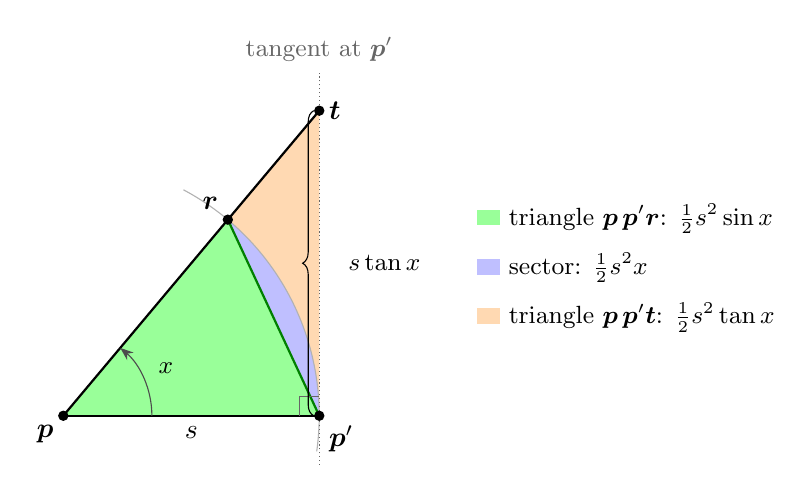
\begin{tikzpicture}[scale=1.25,>=Stealth]
  \def\s{2.6}\def\x{50}
  \coordinate (P) at (0,0);
  \coordinate (A) at (0:\s);            % p'
  \coordinate (Q) at (\x:\s);           % q
  \coordinate (T) at ({\s},{\s*tan(\x)}); % t on the tangent at p'
  \fill[orange!30] (P) -- (A) -- (T) -- cycle;
  \fill[blue!25] (P) -- (A) arc[start angle=0,end angle=\x,radius=\s]
    -- cycle;
  \fill[green!40] (P) -- (A) -- (Q) -- cycle;
  \draw[black!30] (-8:\s) arc[start angle=-8,end angle=\x+12,radius=\s];
  \draw[thick] (P) -- (A) node[pos=0.5,below] {$s$};
  \draw[thick] (P) -- (T);
  \draw[thick,green!50!black] (A) -- (Q);
  \draw[densely dotted,black!60] ($(A)+(0,-0.5)$) -- ($(T)+(0,0.4)$)
    node[above,font=\small,black!60] {tangent at $\p'$};
  \draw[black!60] (A) ++(-0.2,0) -- ++(0,0.2) -- ++(0.2,0);
  \draw[->,black!70] (0.9,0) arc[start angle=0,end angle=\x,radius=0.9];
  \node[font=\small] at (\x/2:1.15) {$x$};
  \fill (P) circle (1.5pt) node[below left] {$\p$};
  \fill (A) circle (1.5pt) node[below right] {$\p'$};
  \fill (Q) circle (1.5pt) node[above left] {$\bm r$};
  \fill (T) circle (1.5pt) node[right] {$\bm t$};
  \draw[decorate,decoration={brace,amplitude=4pt,raise=2pt}]
    (A) -- (T) node[midway,right=7pt,font=\small] {$s\tan x$};
  \node[font=\small,anchor=west] at (4.1,2.0)
    {\tikz\fill[green!40] (0,0) rectangle (0.3,0.2); triangle $\p\,\p'\bm r$:
    $\tfrac12 s^2\sin x$};
  \node[font=\small,anchor=west] at (4.1,1.5)
    {\tikz\fill[blue!25] (0,0) rectangle (0.3,0.2); sector: $\tfrac12 s^2 x$};
  \node[font=\small,anchor=west] at (4.1,1.0)
    {\tikz\fill[orange!30] (0,0) rectangle (0.3,0.2); triangle $\p\,\p'\bm t$:
    $\tfrac12 s^2\tan x$};
\end{tikzpicture}
\caption{The three nested regions behind $\sin x<x<\tan x$. Each contains
the previous one, so their areas increase.}
\label{fig:sinx}
\end{figure}

Take a circle of radius $s$ centred at $\p$, a point $\p'$ on it, and the
point $\bm r$ on the circle seen from $\p$ at the angle $x$ from $\p'$
(\cref{fig:sinx}). Let $\bm t$ be the point where the ray from $\p$ through
$\bm r$ meets the tangent at $\p'$. Three regions are nested:
\begin{itemize}
  \item the triangle $\p\,\p'\,\bm r$, with base $\|\p-\bm r\|=s$ and height
    $s\sin x$ (the distance from $\p'$ to the line $\p\bm r$), so area
    $\tfrac12 s^2\sin x$;
  \item the circular sector $\p\,\p'\,\bm r$, a fraction $x/(2\pi)$ of the
    disc of area $\pi s^2$, so area $\tfrac12 s^2 x$;
  \item the triangle $\p\,\p'\,\bm t$, right-angled at $\p'$ with legs $s$
    and $s\tan x$, so area $\tfrac12 s^2\tan x$.
\end{itemize}
The first is inside the second because the sector is convex (its angle is
less than $\pi$) and contains the three vertices $\p,\p',\bm r$. The second
is inside the third because the whole disc lies on the same side of the
tangent as $\p$: any point $\bm y\ne\p'$ of the tangent satisfies
$\|\bm y-\p\|^2=s^2+\|\bm y-\p'\|^2>s^2$ (Pythagoras, the tangent being
perpendicular to the radius), so the tangent line never enters the disc.
Each inclusion leaves out a region of positive area, so
$\tfrac12 s^2\sin x<\tfrac12 s^2 x<\tfrac12 s^2\tan x$. Dividing by
$\tfrac12 s^2 x$ gives $\sin x/x<1$, and dividing by $\tfrac12 s^2\tan x$
gives $\cos x<\sin x/x$: this is \eqref{eq:sinx}. No derivative or series
is needed; the only analytic input is that the area of a sector is
proportional to its angle, which is how the radian is defined.

\chapter{Bayesian networks and d-separation}
\label{app:bayesnet}

The derivations of \cref{ch:statespace,ch:bayes} repeatedly drop variables
from a conditioning: ``given the current pose, the past does not matter'',
``the next control says nothing about the current pose''. Each of these is
a statement of \emph{conditional independence}. This appendix explains a
way to check such statements without any computation: draw the model as a
graph, and read the independences off the graph.

It proceeds in four steps: what conditional independence means
(\cref{sec:condind}); how a model is drawn as a graph
(\cref{sec:bn}); the three situations that can occur along a path of the
graph, each proved from the definition (\cref{sec:three}); and the
general rule, called \emph{d-separation}, with a recipe to apply it
(\cref{sec:dsep}). \Cref{sec:bayesnet-mower} then applies the recipe to
the mower.

\section{Conditional independence}
\label{sec:condind}

Let $A$, $B$ and $C$ be random variables. $A$ and $B$ are
\emph{independent} if knowing one says nothing about the other:
$p(a\mid b)=p(a)$, or equivalently $p(a,b)=p(a)\,p(b)$. We write
$A\indep B$.

They are \emph{conditionally independent given $C$} if, \emph{once $C$ is
known}, knowing $B$ says nothing more about $A$:
\[
  p(a\mid b,c)=p(a\mid c),\qquad\text{or equivalently}\qquad
  p(a,b\mid c)=p(a\mid c)\,p(b\mid c).
\]
We write $A\indep B\mid C$. This is exactly what allows a variable to be
dropped from a conditioning.

The two notions are different, and neither implies the other. Two
variables can be dependent and become independent once a third is known;
two variables can be independent and become dependent once a third is
known. \Cref{sec:three} gives an example of each.

\section{Bayesian networks}
\label{sec:bn}

A model is often described by saying, for each variable, which other
variables it is computed from. A \emph{Bayesian network} draws this
description: one node per variable, and an arrow $A\rightarrow B$ when $A$
is one of the variables that $B$ is computed from. The arrows must not
form a cycle.

Some vocabulary. In $A\rightarrow B$, $A$ is a \emph{parent} of $B$ and
$B$ a \emph{child} of $A$. The set of parents of a node $v$ is written
$\mathrm{pa}(v)$. The \emph{descendants} of $v$ are its children, their
children, and so on: every node that can be reached from $v$ by following
arrows forwards.

The graph stands for a factorisation of the joint distribution, with one
factor per variable, the distribution of that variable given its parents:
\begin{equation}\label{eq:bnfactor}
  p(v_1,\dots,v_n)=\prod_{k=1}^n p\bigl(v_k\mid\mathrm{pa}(v_k)\bigr).
\end{equation}
A variable without parents contributes its plain distribution $p(v_k)$.

\begin{example}{A garden}{garden}
Four variables: it rained ($R$), the sprinkler was on ($S$), the grass is
wet ($W$), someone slips on the grass ($L$). Rain and sprinkler each make
the grass wet, and wet grass makes people slip (\cref{fig:garden}). The
parents are $\mathrm{pa}(W)=\{R,S\}$ and $\mathrm{pa}(L)=\{W\}$; $R$ and
$S$ have none. The descendants of $R$ are $W$ and $L$. The factorisation
\eqref{eq:bnfactor} reads
\[
  p(r,s,w,l)=p(r)\,p(s)\,p(w\mid r,s)\,p(l\mid w).
\]
\end{example}

\begin{figure}[ht]
\centering
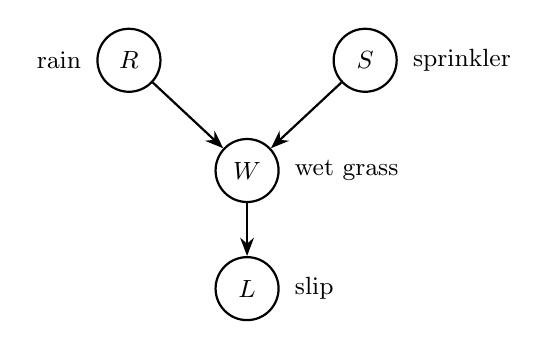
\begin{tikzpicture}[>=Stealth,
  var/.style={circle,draw,thick,minimum size=8mm,inner sep=0pt,font=\small}]
  \node[var] (R) at (0,1.4) {$R$};
  \node[var] (S) at (3,1.4) {$S$};
  \node[var] (W) at (1.5,0) {$W$};
  \node[var] (L) at (1.5,-1.5) {$L$};
  \draw[->,thick] (R) -- (W);
  \draw[->,thick] (S) -- (W);
  \draw[->,thick] (W) -- (L);
  \node[left=2pt,font=\small] at (R.west) {rain};
  \node[right=2pt,font=\small] at (S.east) {sprinkler};
  \node[right=2pt,font=\small] at (W.east) {wet grass};
  \node[right=2pt,font=\small] at (L.east) {slip};
\end{tikzpicture}
\caption{The Bayesian network of \cref{ex:garden}.}
\label{fig:garden}
\end{figure}

For the mower (\cref{fig:bayesnet}), the pose $\x_{t+1}$ is computed from
$\x_t$ and $\uu_t$, and the measurement $\z_t$ from $\x_t$:
$\mathrm{pa}(\x_{t+1})=\{\x_t,\uu_t\}$ and $\mathrm{pa}(\z_t)=\{\x_t\}$.
The factorisation \eqref{eq:bnfactor} is then \eqref{eq:joint}. The
controls are known inputs rather than random variables; they are drawn as
nodes that are always given, and nothing below changes.

\section{The three building blocks}
\label{sec:three}

Take three variables $A$, $B$, $C$ with an arrow between $A$ and $B$ and
an arrow between $B$ and $C$, and no arrow between $A$ and $C$. The two
arrows can be oriented in three essentially different ways
(\cref{fig:connections}). In each case the question is the same: are $A$
and $C$ independent, and does the answer change when $B$ is known?

\begin{figure}[ht]
\centering
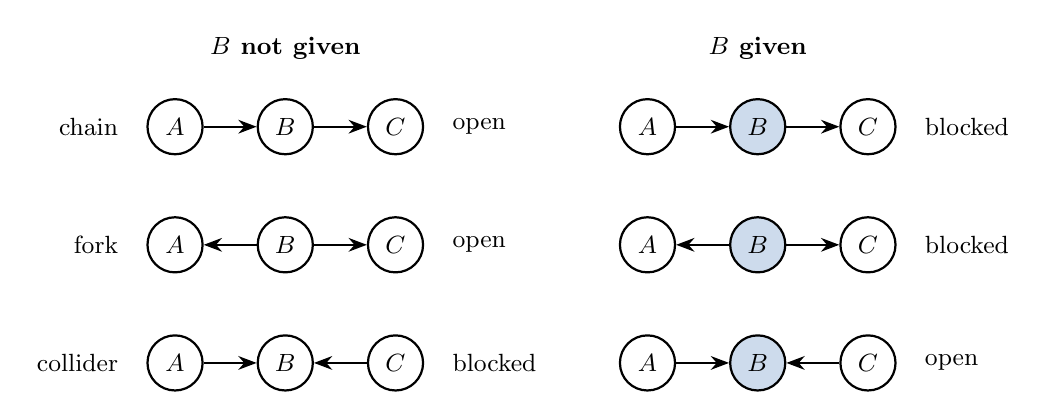
\begin{tikzpicture}[>=Stealth,
  var/.style={circle,draw,thick,minimum size=7mm,inner sep=0pt,font=\small,
    fill=white},
  giv/.style={fill=defblue!22}]
  \node[font=\small\bfseries] at (2.6,1.0) {$B$ not given};
  \node[font=\small\bfseries] at (8.6,1.0) {$B$ given};
  \foreach \row/\name/\ta/\tb/\va/\vb in {
      0/chain/->/->/open/blocked,
      -1.5/fork/<-/->/open/blocked,
      -3.0/collider/->/<-/blocked/open}{
    \node[font=\small,anchor=east] at (0.6,\row) {\name};
    \foreach \dx/\st/\verdict in {1.2/{}/\va, 7.2/giv/\vb}{
      \node[var] (A) at (\dx,\row) {$A$};
      \node[var,\st] (B) at (\dx+1.4,\row) {$B$};
      \node[var] (C) at (\dx+2.8,\row) {$C$};
      \draw[\ta,thick] (A) -- (B);
      \draw[\tb,thick] (B) -- (C);
      \node[font=\small,anchor=west] at (\dx+3.4,\row) {\verdict};
    }
  }
\end{tikzpicture}
\caption{The three ways two arrows can meet at a middle node $B$, and
whether information passes between $A$ and $C$ (``open'') or not
(``blocked''). A shaded node is given. Chains and forks are open until $B$
is given; a collider is the other way round.}
\label{fig:connections}
\end{figure}

\subsection*{Chain: $A\rightarrow B\rightarrow C$}

\emph{Example.} It rains ($A$), so the grass is wet ($B$), so someone slips
($C$). Rain makes slipping more likely: $A$ and $C$ are dependent. But if
we already know whether the grass is wet, learning that it rained tells
nothing more about slipping, because rain acts on slipping only through
the wet grass.

\emph{Statement.} In a chain, $A$ and $C$ are in general dependent, and
$A\indep C\mid B$.

\emph{Proof.} The factorisation \eqref{eq:bnfactor} is
$p(a,b,c)=p(a)\,p(b\mid a)\,p(c\mid b)$. Its first two factors multiply to
$p(a,b)$, so
\[
  p(c\mid a,b)=\frac{p(a,b,c)}{p(a,b)}=p(c\mid b).
\]
Given $B$, the value of $A$ does not change the distribution of $C$.

\subsection*{Fork: $A\leftarrow B\rightarrow C$}

\emph{Example.} A patient has the flu ($B$), which causes fever ($A$) and
cough ($C$). In the population, fever and cough go together: seeing one
makes the other more likely, because it makes the flu more likely. Among
patients known to have the flu, a fever says nothing more about a cough.

\emph{Statement.} In a fork, $A$ and $C$ are in general dependent, and
$A\indep C\mid B$.

\emph{Proof.} The factorisation is $p(a,b,c)=p(b)\,p(a\mid b)\,p(c\mid b)$.
Dividing by $p(b)$,
\[
  p(a,c\mid b)=p(a\mid b)\,p(c\mid b).
\]

In both cases the given middle node is said to \emph{screen off} $A$ from
$C$.

\subsection*{Collider: $A\rightarrow B\leftarrow C$}

\emph{Example.} Rain ($A$) and the sprinkler ($C$) both wet the grass
($B$). Rain and sprinkler have nothing to do with each other: they are
independent. Now suppose we see that the grass is wet. If we then learn
that the sprinkler was on, rain becomes \emph{less} likely, because the
sprinkler already explains the wet grass. Once the common effect is known,
its two causes are no longer independent. This is called \emph{explaining
away}.

\emph{Statement.} In a collider, $A\indep C$, and in general $A$ and $C$
are dependent given $B$.

\emph{Proof.} The factorisation is $p(a,b,c)=p(a)\,p(c)\,p(b\mid a,c)$.
Summing over $b$, and using $\sum_bp(b\mid a,c)=1$,
\[
  p(a,c)=p(a)\,p(c):
\]
$A$ and $C$ are independent. Given $B$, however,
$p(a,c\mid b)=p(a)\,p(c)\,p(b\mid a,c)/p(b)$, and the factor
$p(b\mid a,c)$ ties $a$ and $c$ together; the next example shows that the
dependence is real.

\begin{example}{Explaining away, with numbers}{explain}
It rains with probability $0.2$, the sprinkler is on with probability
$0.2$, independently, and the grass is wet exactly when at least one of
the two happened. The grass is wet with probability $1-0.8\times0.8=0.36$.
\begin{itemize}[nosep]
  \item Knowing only that the grass is wet, the probability of rain is
    $0.2/0.36=0.56$.
  \item Knowing that the grass is wet \emph{and} that the sprinkler was on,
    the grass would be wet whether it rained or not, so the wet grass says
    nothing about rain: its probability is back to $0.2$.
\end{itemize}
Given the wet grass, learning about the sprinkler changes the probability
of rain from $0.56$ to $0.2$: the two causes are dependent.
\end{example}

One more fact about colliders: knowing a \emph{descendant} of the collider
has the same effect as knowing the collider. If we do not see the grass
but see someone slip on it, the grass is probably wet, and rain and
sprinkler become dependent again.

\begin{inwords}
Information flows through a chain or a fork, unless the middle node is
known. Information does not flow through a collider, unless the collider,
or something it causes, is known.
\end{inwords}

\section{d-separation}
\label{sec:dsep}

In a larger graph, two variables can be connected by several routes, each
made of chains, forks and colliders. The rule of d-separation (``d'' for
\emph{directional}) combines the three building blocks.

A \emph{path} between two nodes is a sequence of nodes in which each one is
joined to the next by an arrow, \emph{whatever the direction of the
arrows}. In \cref{fig:garden}, $R\rightarrow W\leftarrow S$ is a path from
$R$ to $S$, although no arrow leads from $R$ to $S$. Each intermediate node
of a path is a chain, a fork or a collider \emph{on that path}, according
to the two arrows of the path that meet at it.

\begin{definition}{Blocked path, d-separation}{dsep}
Let $\mathcal S$ be a set of given variables. A path is \emph{blocked} by
$\mathcal S$ if at least one of its intermediate nodes $B$ satisfies one
of the following:
\begin{itemize}[nosep]
  \item $B$ is a chain or a fork on the path, and $B$ is in $\mathcal S$;
  \item $B$ is a collider on the path, and neither $B$ nor any descendant
    of $B$ is in $\mathcal S$.
\end{itemize}
A path that is not blocked is \emph{open}. Two variables $X$ and $Y$ are
\emph{d-separated} by $\mathcal S$ if every path between them is blocked
by $\mathcal S$.
\end{definition}

One blocking node is enough to block a path, but every path must be
blocked for d-separation.

\begin{theorem}{d-separation implies conditional independence}{dsep}
If $X$ and $Y$ are d-separated by $\mathcal S$ in a Bayesian network, then
$X\indep Y\mid\mathcal S$ for every distribution that factorises as
\eqref{eq:bnfactor}.
\end{theorem}

The proofs of \cref{sec:three} are the three smallest cases of this
theorem. The general proof extends the same computations to any graph;
it can be found in Koller and Friedman (see the references).

\paragraph{A recipe.} To decide whether $X\indep Y\mid\mathcal S$:
\begin{enumerate}[nosep]
  \item Shade the nodes of $\mathcal S$.
  \item List the paths between $X$ and $Y$, ignoring the direction of the
    arrows.
  \item On each path, look for a blocking node: a shaded chain or fork
    node, or a collider that is unshaded and has no shaded descendant.
  \item If every path has a blocking node, $X$ and $Y$ are independent
    given $\mathcal S$. If some path has none, the graph does not
    guarantee independence.
\end{enumerate}

\begin{example}{Three questions about the garden}{gardenq}
In \cref{fig:garden}:
\begin{itemize}[nosep]
  \item \emph{Is $R\indep S$, with nothing given?} The only path is
    $R\rightarrow W\leftarrow S$. Its middle node $W$ is a collider; it is
    not given, and neither is its descendant $L$. The path is blocked:
    yes, rain and sprinkler are independent.
  \item \emph{Is $R\indep S\mid L$?} Same path, but now $L$, a descendant
    of the collider $W$, is given. The path is open: no.
  \item \emph{Is $R\indep L\mid W$?} The only path is
    $R\rightarrow W\rightarrow L$, a chain whose middle node $W$ is given.
    The path is blocked: yes. Once the state of the grass is known, rain
    says nothing more about slipping.
\end{itemize}
\end{example}

\section{Reading the mower's network}
\label{sec:bayesnet-mower}

The recipe is now applied to the four statements that the book relies on.
Each is drawn on four consecutive steps of the network of
\cref{fig:bayesnet}; the rest of the chain, to the left and to the right,
only adds paths that pass through the same nodes. In each drawing the
shaded nodes are given, the nodes with an orange ring are the two whose
independence is in question, and a coloured band marks a path between
them: red if it is blocked, green if it is open.

Two features of this network do most of the work. First, a measurement
$\z_t$ has a single neighbour, its parent $\x_t$. Second, the poses form a
chain, so that the past and the future are joined only through the
current pose.

\subsection*{(a) Assumption \ref{A2}: the measurement depends only on the
current pose}

\emph{Claim.} $p(\z_t\mid\x_{0:t},\uu_{0:t-1},\z_{1:t-1})=p(\z_t\mid\x_t)$:
given $\x_t$, the measurement $\z_t$ is independent of all the earlier
poses, controls and measurements.

\begin{center}
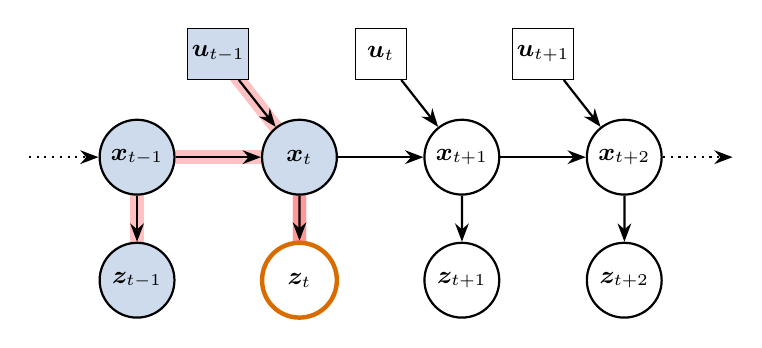
\begin{tikzpicture}[scale=1.25,>=Stealth,
  var/.style={circle,draw,thick,minimum size=9.5mm,inner sep=0pt,fill=white,font=\small},
  ctl/.style={rectangle,draw,minimum size=6.5mm,inner sep=1.5pt,fill=white,font=\small},
  giv/.style={fill=defblue!22},
  qry/.style={draw=orange!85!black,line width=1.6pt}]
  \draw[line width=5pt,red!70,opacity=0.35,line cap=round,line join=round] (0.000,-1.250) -- (0.000,0.000) -- (1.650,0.000) -- (1.650,-1.250);
  \draw[line width=5pt,red!70,opacity=0.35,line cap=round,line join=round] (0.825,1.050) -- (1.650,0.000) -- (1.650,-1.250);
  \node[var,giv] (x0) at (0.000,0.000) {$\x_{t-1}$};
  \node[var,giv] (x1) at (1.650,0.000) {$\x_{t}$};
  \node[var] (x2) at (3.300,0.000) {$\x_{t+1}$};
  \node[var] (x3) at (4.950,0.000) {$\x_{t+2}$};
  \node[var,giv] (z0) at (0.000,-1.250) {$\z_{t-1}$};
  \node[var,qry] (z1) at (1.650,-1.250) {$\z_{t}$};
  \node[var] (z2) at (3.300,-1.250) {$\z_{t+1}$};
  \node[var] (z3) at (4.950,-1.250) {$\z_{t+2}$};
  \node[ctl,giv] (u0) at (0.825,1.050) {$\uu_{t-1}$};
  \node[ctl] (u1) at (2.475,1.050) {$\uu_{t}$};
  \node[ctl] (u2) at (4.125,1.050) {$\uu_{t+1}$};
  \draw[->,thick] (x0) -- (x1);
  \draw[->,thick] (x1) -- (x2);
  \draw[->,thick] (x2) -- (x3);
  \draw[->,thick] (u0) -- (x1);
  \draw[->,thick] (u1) -- (x2);
  \draw[->,thick] (u2) -- (x3);
  \draw[->,thick] (x0) -- (z0);
  \draw[->,thick] (x1) -- (z1);
  \draw[->,thick] (x2) -- (z2);
  \draw[->,thick] (x3) -- (z3);
  \draw[->,thick,dotted] ($(x0)+(-1.1,0)$) -- (x0);
  \draw[->,thick,dotted] (x3) -- ++(1.1,0);
\end{tikzpicture}

\end{center}

\emph{Check.} Every path that reaches $\z_t$ ends with the arrow
$\x_t\rightarrow\z_t$, because $\x_t$ is its only neighbour. On such a
path $\x_t$ is an intermediate node with an arrow leaving towards $\z_t$,
so it is a chain node (if the path arrives from $\x_{t-1}$ or
$\uu_{t-1}$) or a fork node (if it arrives from $\x_{t+1}$), never a
collider. It is given, so every path is blocked. The drawing shows two of
them, from $\z_{t-1}$ and from $\uu_{t-1}$.

\subsection*{(b) Assumption \ref{A1}: the next pose depends only on the
current pose and control}

\emph{Claim.} $p(\x_{t+1}\mid\x_{0:t},\uu_{0:t},\z_{1:t})=
p(\x_{t+1}\mid\x_t,\uu_t)$: given $\x_t$ and $\uu_t$, the next pose is
independent of the earlier poses $\x_{0:t-1}$, the earlier controls
$\uu_{0:t-1}$ and the measurements $\z_{1:t}$.

\begin{center}
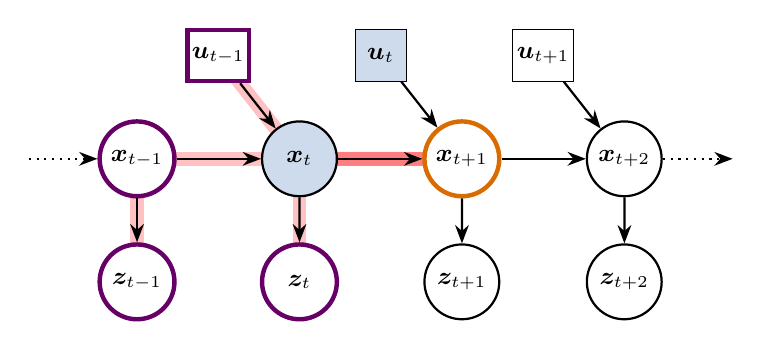
\begin{tikzpicture}[scale=1.25,>=Stealth,
  var/.style={circle,draw,thick,minimum size=9.5mm,inner sep=0pt,fill=white,font=\small},
  ctl/.style={rectangle,draw,minimum size=6.5mm,inner sep=1.5pt,fill=white,font=\small},
  giv/.style={fill=defblue!22},
  qry/.style={draw=orange!85!black,line width=1.6pt},
  drp/.style={draw=violet!80!black,line width=1.6pt}]
  \draw[line width=5pt,red!70,opacity=0.35,line cap=round,line join=round] (0.000,-1.250) -- (0.000,0.000) -- (1.650,0.000) -- (3.300,0.000);
  \draw[line width=5pt,red!70,opacity=0.35,line cap=round,line join=round] (1.650,-1.250) -- (1.650,0.000) -- (3.300,0.000);
  \draw[line width=5pt,red!70,opacity=0.35,line cap=round,line join=round] (0.825,1.050) -- (1.650,0.000) -- (3.300,0.000);
  \node[var,drp] (x0) at (0.000,0.000) {$\x_{t-1}$};
  \node[var,giv] (x1) at (1.650,0.000) {$\x_{t}$};
  \node[var,qry] (x2) at (3.300,0.000) {$\x_{t+1}$};
  \node[var] (x3) at (4.950,0.000) {$\x_{t+2}$};
  \node[var,drp] (z0) at (0.000,-1.250) {$\z_{t-1}$};
  \node[var,drp] (z1) at (1.650,-1.250) {$\z_{t}$};
  \node[var] (z2) at (3.300,-1.250) {$\z_{t+1}$};
  \node[var] (z3) at (4.950,-1.250) {$\z_{t+2}$};
  \node[ctl,drp] (u0) at (0.825,1.050) {$\uu_{t-1}$};
  \node[ctl,giv] (u1) at (2.475,1.050) {$\uu_{t}$};
  \node[ctl] (u2) at (4.125,1.050) {$\uu_{t+1}$};
  \draw[->,thick] (x0) -- (x1);
  \draw[->,thick] (x1) -- (x2);
  \draw[->,thick] (x2) -- (x3);
  \draw[->,thick] (u0) -- (x1);
  \draw[->,thick] (u1) -- (x2);
  \draw[->,thick] (u2) -- (x3);
  \draw[->,thick] (x0) -- (z0);
  \draw[->,thick] (x1) -- (z1);
  \draw[->,thick] (x2) -- (z2);
  \draw[->,thick] (x3) -- (z3);
  \draw[->,thick,dotted] ($(x0)+(-1.1,0)$) -- (x0);
  \draw[->,thick,dotted] (x3) -- ++(1.1,0);
\end{tikzpicture}

\end{center}

\emph{Check.} Each of the variables to drop is joined to the rest of the
graph only through $\x_t$. So every path from one of them to $\x_{t+1}$
passes through $\x_t$ and leaves it by the arrow
$\x_t\rightarrow\x_{t+1}$: there $\x_t$ is a chain node
($\x_{t-1}\rightarrow\x_t\rightarrow\x_{t+1}$) or a fork node
($\z_t\leftarrow\x_t\rightarrow\x_{t+1}$). It is given, so every path is
blocked.

\subsection*{(c) Prediction: the next control says nothing about the
current pose}

\emph{Claim.} $p(\x_t\mid\z_{1:t},\uu_{0:t})=p(\x_t\mid\z_{1:t},
\uu_{0:t-1})$: given the measurements and the earlier controls, $\x_t$ is
independent of $\uu_t$. This is the step of the proof of \cref{thm:bayes}
that turns the second factor into $\bel(\x_t)$.

\begin{center}
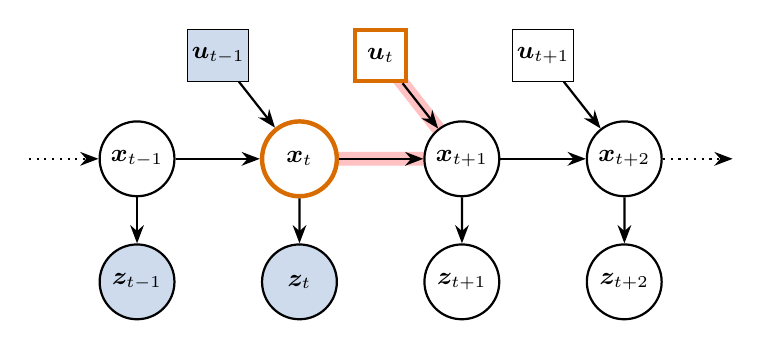
\begin{tikzpicture}[scale=1.25,>=Stealth,
  var/.style={circle,draw,thick,minimum size=9.5mm,inner sep=0pt,fill=white,font=\small},
  ctl/.style={rectangle,draw,minimum size=6.5mm,inner sep=1.5pt,fill=white,font=\small},
  giv/.style={fill=defblue!22},
  qry/.style={draw=orange!85!black,line width=1.6pt}]
  \draw[line width=5pt,red!70,opacity=0.35,line cap=round,line join=round] (1.650,0.000) -- (3.300,0.000) -- (2.475,1.050);
  \node[var] (x0) at (0.000,0.000) {$\x_{t-1}$};
  \node[var,qry] (x1) at (1.650,0.000) {$\x_{t}$};
  \node[var] (x2) at (3.300,0.000) {$\x_{t+1}$};
  \node[var] (x3) at (4.950,0.000) {$\x_{t+2}$};
  \node[var,giv] (z0) at (0.000,-1.250) {$\z_{t-1}$};
  \node[var,giv] (z1) at (1.650,-1.250) {$\z_{t}$};
  \node[var] (z2) at (3.300,-1.250) {$\z_{t+1}$};
  \node[var] (z3) at (4.950,-1.250) {$\z_{t+2}$};
  \node[ctl,giv] (u0) at (0.825,1.050) {$\uu_{t-1}$};
  \node[ctl,qry] (u1) at (2.475,1.050) {$\uu_{t}$};
  \node[ctl] (u2) at (4.125,1.050) {$\uu_{t+1}$};
  \draw[->,thick] (x0) -- (x1);
  \draw[->,thick] (x1) -- (x2);
  \draw[->,thick] (x2) -- (x3);
  \draw[->,thick] (u0) -- (x1);
  \draw[->,thick] (u1) -- (x2);
  \draw[->,thick] (u2) -- (x3);
  \draw[->,thick] (x0) -- (z0);
  \draw[->,thick] (x1) -- (z1);
  \draw[->,thick] (x2) -- (z2);
  \draw[->,thick] (x3) -- (z3);
  \draw[->,thick,dotted] ($(x0)+(-1.1,0)$) -- (x0);
  \draw[->,thick,dotted] (x3) -- ++(1.1,0);
\end{tikzpicture}

\end{center}

\emph{Check.} The only arrow at $\uu_t$ is $\uu_t\rightarrow\x_{t+1}$, so
every path from $\uu_t$ starts with it. To reach $\x_t$, the path must
then come back along $\x_{t+1}\leftarrow\x_t$: the two arrows point into
$\x_{t+1}$, which is a collider. Neither $\x_{t+1}$ nor any of its
descendants ($\z_{t+1}$, $\x_{t+2}$, \dots) is given, since only
measurements up to time $t$ are. The path is blocked. A path that
continues from $\x_{t+1}$ into the future cannot return to $\x_t$ without
passing through $\x_{t+1}$ a second time, so there is no other path.

The same argument shows that all the future controls are independent of
the past poses, which is used in the proof of \cref{prop:joint}.

\subsection*{(d) Smoothing: a later measurement does say something about
an earlier pose}

\emph{Question.} Given the measurements up to time $t$, is $\x_t$
independent of the next measurement $\z_{t+1}$?

\begin{center}
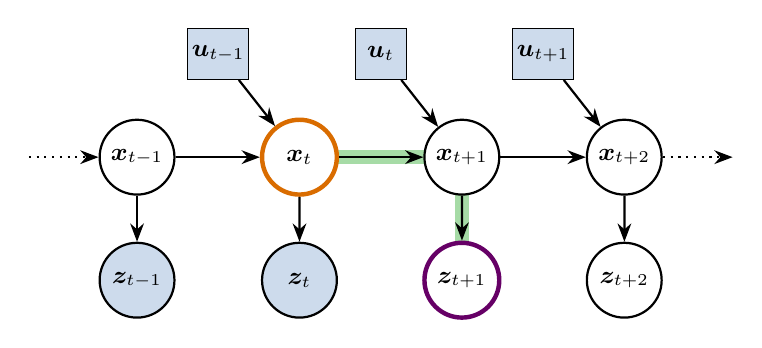
\begin{tikzpicture}[scale=1.25,>=Stealth,
  var/.style={circle,draw,thick,minimum size=9.5mm,inner sep=0pt,fill=white,font=\small},
  ctl/.style={rectangle,draw,minimum size=6.5mm,inner sep=1.5pt,fill=white,font=\small},
  giv/.style={fill=defblue!22},
  qry/.style={draw=orange!85!black,line width=1.6pt},
  drp/.style={draw=violet!80!black,line width=1.6pt}]
  \draw[line width=5pt,green!60!black,opacity=0.35,line cap=round,line join=round] (1.650,0.000) -- (3.300,0.000) -- (3.300,-1.250);
  \node[var] (x0) at (0.000,0.000) {$\x_{t-1}$};
  \node[var,qry] (x1) at (1.650,0.000) {$\x_{t}$};
  \node[var] (x2) at (3.300,0.000) {$\x_{t+1}$};
  \node[var] (x3) at (4.950,0.000) {$\x_{t+2}$};
  \node[var,giv] (z0) at (0.000,-1.250) {$\z_{t-1}$};
  \node[var,giv] (z1) at (1.650,-1.250) {$\z_{t}$};
  \node[var,drp] (z2) at (3.300,-1.250) {$\z_{t+1}$};
  \node[var] (z3) at (4.950,-1.250) {$\z_{t+2}$};
  \node[ctl,giv] (u0) at (0.825,1.050) {$\uu_{t-1}$};
  \node[ctl,giv] (u1) at (2.475,1.050) {$\uu_{t}$};
  \node[ctl,giv] (u2) at (4.125,1.050) {$\uu_{t+1}$};
  \draw[->,thick] (x0) -- (x1);
  \draw[->,thick] (x1) -- (x2);
  \draw[->,thick] (x2) -- (x3);
  \draw[->,thick] (u0) -- (x1);
  \draw[->,thick] (u1) -- (x2);
  \draw[->,thick] (u2) -- (x3);
  \draw[->,thick] (x0) -- (z0);
  \draw[->,thick] (x1) -- (z1);
  \draw[->,thick] (x2) -- (z2);
  \draw[->,thick] (x3) -- (z3);
  \draw[->,thick,dotted] ($(x0)+(-1.1,0)$) -- (x0);
  \draw[->,thick,dotted] (x3) -- ++(1.1,0);
\end{tikzpicture}

\end{center}

\emph{Check.} The path $\x_t\rightarrow\x_{t+1}\rightarrow\z_{t+1}$ is a
chain whose middle node $\x_{t+1}$ is not given. Nothing blocks it: the
path is open, and the graph does not give independence. Indeed $\z_{t+1}$
is a measurement of $\x_{t+1}$, which is one step away from $\x_t$. A
filter ignores this information about the past; a smoother uses it
(\cref{sec:smoothing}).

\subsection*{Complement: controls computed during the run}

In the network of \cref{fig:bayesnet} no arrow enters a control: the
controls are fixed in advance. A mower can also compute them as it goes,
for instance to steer back towards its planned path. What this changes
depends on what the controls are computed from. In the two drawings below
the new arrows are blue.

\emph{From the past measurements.} If $\uu_t$ is computed from
$\z_{1:t}$, arrows go from the measurements to the controls (only the
arrow from the latest measurement is drawn).

\begin{center}
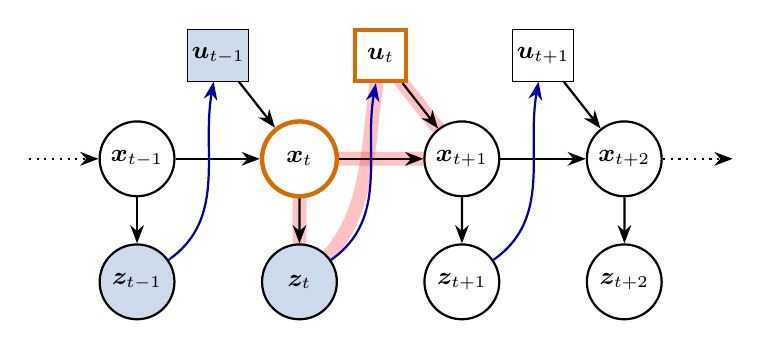
\begin{tikzpicture}[scale=1.25,>=Stealth,
  var/.style={circle,draw,thick,minimum size=9.5mm,inner sep=0pt,fill=white,font=\small},
  ctl/.style={rectangle,draw,minimum size=6.5mm,inner sep=1.5pt,fill=white,font=\small},
  giv/.style={fill=defblue!22},
  qry/.style={draw=orange!85!black,line width=1.6pt}]
  \draw[line width=5pt,red!70,opacity=0.35,line cap=round,line join=round] (1.650,0.000) -- (3.300,0.000) -- (2.475,1.050);
  \draw[line width=5pt,red!70,opacity=0.35,line cap=round,line join=round] (1.650,0.000) -- (1.650,-1.250) to[out=35,in=-100] (2.475,1.050);
  \node[var] (x0) at (0.000,0.000) {$\x_{t-1}$};
  \node[var,qry] (x1) at (1.650,0.000) {$\x_{t}$};
  \node[var] (x2) at (3.300,0.000) {$\x_{t+1}$};
  \node[var] (x3) at (4.950,0.000) {$\x_{t+2}$};
  \node[var,giv] (z0) at (0.000,-1.250) {$\z_{t-1}$};
  \node[var,giv] (z1) at (1.650,-1.250) {$\z_{t}$};
  \node[var] (z2) at (3.300,-1.250) {$\z_{t+1}$};
  \node[var] (z3) at (4.950,-1.250) {$\z_{t+2}$};
  \node[ctl,giv] (u0) at (0.825,1.050) {$\uu_{t-1}$};
  \node[ctl,qry] (u1) at (2.475,1.050) {$\uu_{t}$};
  \node[ctl] (u2) at (4.125,1.050) {$\uu_{t+1}$};
  \draw[->,thick] (x0) -- (x1);
  \draw[->,thick] (x1) -- (x2);
  \draw[->,thick] (x2) -- (x3);
  \draw[->,thick] (u0) -- (x1);
  \draw[->,thick] (u1) -- (x2);
  \draw[->,thick] (u2) -- (x3);
  \draw[->,thick] (x0) -- (z0);
  \draw[->,thick] (x1) -- (z1);
  \draw[->,thick] (x2) -- (z2);
  \draw[->,thick] (x3) -- (z3);
  \draw[->,thick,dotted] ($(x0)+(-1.1,0)$) -- (x0);
  \draw[->,thick,dotted] (x3) -- ++(1.1,0);
  \draw[->,thick,blue!70!black] (z0) to[out=35,in=-100] (u0);
  \draw[->,thick,blue!70!black] (z1) to[out=35,in=-100] (u1);
  \draw[->,thick,blue!70!black] (z2) to[out=35,in=-100] (u2);
\end{tikzpicture}

\end{center}

Statement (c) still holds. There is a new path from $\uu_t$ to $\x_t$,
namely $\uu_t\leftarrow\z_t\leftarrow\x_t$, in which $\z_t$ is a chain
node. It is given, so the path is blocked; the same holds for a path
through an earlier measurement. The filter is therefore unchanged: it does
not matter how the controls were chosen, as long as they are computed from
measurements that the filter is given.

One thing does change. A \emph{later} control now carries information
about the past: the path $\uu_{t+1}\leftarrow\z_{t+1}\leftarrow\x_{t+1}$
is open as long as $\z_{t+1}$ is not given. The step of the proof of
\cref{prop:joint} that removes the later controls is then not valid. The
product \eqref{eq:joint} is still the joint density of the poses and the
measurements, with each $\uu_t$ replaced by its expression in terms of
$\z_{1:t}$, but it can no longer be read as a density given the whole
sequence of controls.

\emph{From the true pose.} If $\uu_t$ is computed from $\x_t$ itself,
there is an arrow $\x_t\rightarrow\uu_t$.

\begin{center}
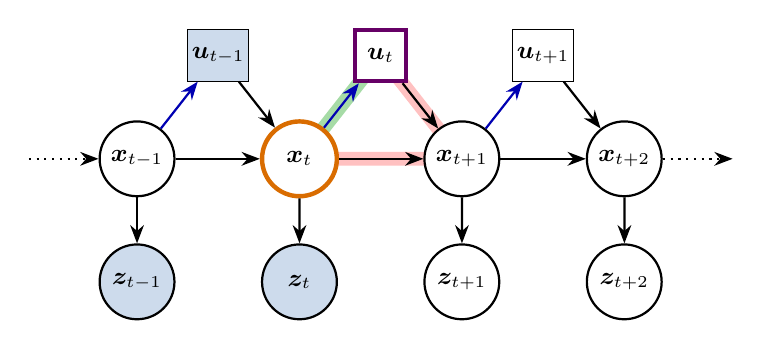
\begin{tikzpicture}[scale=1.25,>=Stealth,
  var/.style={circle,draw,thick,minimum size=9.5mm,inner sep=0pt,fill=white,font=\small},
  ctl/.style={rectangle,draw,minimum size=6.5mm,inner sep=1.5pt,fill=white,font=\small},
  giv/.style={fill=defblue!22},
  qry/.style={draw=orange!85!black,line width=1.6pt},
  drp/.style={draw=violet!80!black,line width=1.6pt}]
  \draw[line width=5pt,red!70,opacity=0.35,line cap=round,line join=round] (1.650,0.000) -- (3.300,0.000) -- (2.475,1.050);
  \draw[line width=5pt,green!60!black,opacity=0.35,line cap=round,line join=round] (1.650,0.000) -- (2.475,1.050);
  \node[var] (x0) at (0.000,0.000) {$\x_{t-1}$};
  \node[var,qry] (x1) at (1.650,0.000) {$\x_{t}$};
  \node[var] (x2) at (3.300,0.000) {$\x_{t+1}$};
  \node[var] (x3) at (4.950,0.000) {$\x_{t+2}$};
  \node[var,giv] (z0) at (0.000,-1.250) {$\z_{t-1}$};
  \node[var,giv] (z1) at (1.650,-1.250) {$\z_{t}$};
  \node[var] (z2) at (3.300,-1.250) {$\z_{t+1}$};
  \node[var] (z3) at (4.950,-1.250) {$\z_{t+2}$};
  \node[ctl,giv] (u0) at (0.825,1.050) {$\uu_{t-1}$};
  \node[ctl,drp] (u1) at (2.475,1.050) {$\uu_{t}$};
  \node[ctl] (u2) at (4.125,1.050) {$\uu_{t+1}$};
  \draw[->,thick] (x0) -- (x1);
  \draw[->,thick] (x1) -- (x2);
  \draw[->,thick] (x2) -- (x3);
  \draw[->,thick] (u0) -- (x1);
  \draw[->,thick] (u1) -- (x2);
  \draw[->,thick] (u2) -- (x3);
  \draw[->,thick] (x0) -- (z0);
  \draw[->,thick] (x1) -- (z1);
  \draw[->,thick] (x2) -- (z2);
  \draw[->,thick] (x3) -- (z3);
  \draw[->,thick,dotted] ($(x0)+(-1.1,0)$) -- (x0);
  \draw[->,thick,dotted] (x3) -- ++(1.1,0);
  \draw[->,thick,blue!70!black] (x0) -- (u0);
  \draw[->,thick,blue!70!black] (x1) -- (u1);
  \draw[->,thick,blue!70!black] (x2) -- (u2);
\end{tikzpicture}

\end{center}

This arrow is a path between $\x_t$ and $\uu_t$ with no node in between,
so nothing can block it: statement (c) fails. The control is then a kind
of measurement of the pose, and a filter that drops $\uu_t$ in its
prediction step, as in the proof of \cref{thm:bayes}, leaves that
information unused. Assumptions \ref{A1} and \ref{A2} themselves still
hold, because the noises $\bepsilon_t$ and $\vv_t$ remain independent of
everything that came before.

\begin{mower}
The simulations of this book are in the second case at some steps. The
mower follows a path fixed in advance, but near the edge of the lawn the
pilot of the simulation, which knows the true pose, adds a turn towards
the centre. At those steps the commanded control says ``the mower is near
the edge'', and the filters do not use this: there they are not exactly
the Bayes filter of \cref{thm:bayes}, but a filter that ignores part of
what it is told.
\end{mower}

\chapter{Differentiating under the integral sign}
\label{app:feynman}

Exercise~\ref{ex:ecos} needs $\E[\cos\theta]$ for a Gaussian angle
$\theta$, and its solution finds it by a device that is hard to invent
on the spot: put a parameter $a$ into the integral, differentiate with
respect to $a$, and solve the equation that comes out. The device is
classical. Richard Feynman made it popular under the name
\emph{differentiating under the integral sign}; he had learned it as a
student from Woods' \emph{Advanced Calculus}, and it is now often called
\emph{Feynman's trick}. This appendix states the rule that makes it legal
(\cref{sec:feyn-rule}), describes the device (\cref{sec:feyn-idea}),
works three examples of the two ways it closes
(\cref{sec:feyn-easy,sec:feyn-ode}), gives the shorter route to
$\E[\cos\theta]$ through complex numbers (\cref{sec:feyn-complex}), and
ends with how to choose the parameter (\cref{sec:feyn-choose}).

\section{The rule}
\label{sec:feyn-rule}

All the integrals below are integrals of integrable functions, that is,
Lebesgue integrals, and expectations are integrals of this kind. The
rule is a consequence of dominated convergence.

\begin{proposition}{Differentiation under the integral sign}{diffint}
Let $J$ be an open interval, $S$ a subset of $\R$, and
$f:J\times S\to\R$ a function such that
\begin{enumerate}[nosep]
  \item for each $a\in J$, the function $x\mapsto f(a,x)$ is integrable
        on $S$;
  \item for each $x\in S$, the function $a\mapsto f(a,x)$ is
        differentiable on $J$;
  \item there is an integrable function $g$ on $S$ with
        $\abs{\partial_af(a,x)}\le g(x)$ for all $a\in J$ and $x\in S$.
\end{enumerate}
Then $F(a)=\int_Sf(a,x)\,\mathrm dx$ is differentiable on $J$, and
\[
  F'(a)=\int_S\partial_af(a,x)\,\mathrm dx .
\]
\end{proposition}

\begin{proof}
Fix $a\in J$ and a sequence $h_n\to0$ with $h_n\neq0$ and
$a+h_n\in J$. The difference quotient of $F$ is the integral of the
difference quotients of $f$:
\[
  \frac{F(a+h_n)-F(a)}{h_n}=\int_Sq_n(x)\,\mathrm dx,
  \qquad
  q_n(x)=\frac{f(a+h_n,x)-f(a,x)}{h_n}.
\]
For each $x$, $q_n(x)\to\partial_af(a,x)$ by (2), so $\partial_af(a,\cdot)$
is measurable as a limit of measurable functions. By the mean value
theorem, $q_n(x)=\partial_af(\xi_n,x)$ for some $\xi_n$ between $a$ and
$a+h_n$, so $\abs{q_n(x)}\le g(x)$ by (3). Dominated convergence then
gives $\int_Sq_n\to\int_S\partial_af(a,x)\,\mathrm dx$. Write $L=\int_S\partial_af(a,x)\,\mathrm dx$. We have shown: for every
sequence $h_n\to0$ with $h_n\neq0$ and $a+h_n\in J$, the difference
quotient $\bigl(F(a+h_n)-F(a)\bigr)/h_n$ tends to $L$.

It remains to pass from sequences to the limit as $h\to0$, which is what
differentiability asks for; sequences were needed because dominated
convergence is a statement about sequences. Suppose that the quotient $\bigl(F(a+h)-F(a)\bigr)/h$ did not tend to $L$
as $h\to0$. Then there would be an $\varepsilon>0$ such
that, however small $\delta>0$, some $h$ with $0<\abs h<\delta$ and
$a+h\in J$ gives $\bigl|\bigl(F(a+h)-F(a)\bigr)/h-L\bigr|\ge\varepsilon$.
Taking $\delta=1/n$ for $n=1,2,\dots$ gives such an $h_n$ for each $n$:
a sequence with $h_n\to0$, $h_n\neq0$, $a+h_n\in J$, whose quotients all
stay at distance at least $\varepsilon$ from $L$, and so do not tend to
$L$. This contradicts what was shown. So the quotient tends to $L$ as
$h\to0$: $F$ is differentiable at $a$, and $F'(a)=L$, the stated
derivative. Since $a$ was any point of $J$, this holds on all of $J$.
\end{proof}

A complex-valued $f$ is handled by applying the proposition to its real
and imaginary parts. The companion book proves a more general form, with
a parameter in a normed space and a Lipschitz bound in place of (3)
(Theorem~17.20 there).

\emph{Hypothesis (3) is the one to check.} Hypotheses (1) and (2) are
about one $a$, or one $x$, at a time, and they are usually clear.
Hypothesis (3) asks for more: a single integrable function $g$ that bounds
$\partial_af(a,\cdot)$ for \emph{all} $a\in J$ at once. It forbids the
derivative from carrying its mass off to infinity as $a$ varies, and that
can happen.

\emph{An example where (3) fails.} Take $J=(-1,1)$, $S=(0,\infty)$ and
\[
  f(a,x)=a^3x\,e^{-a^2x^2}.
\]
Hypotheses (1) and (2) hold: for each $a$ the function of $x$ is
integrable, and for each $x$ the function of $a$ is differentiable. For
$a\neq0$,
\[
  F(a)=a^3\int_0^\infty x\,e^{-a^2x^2}\,\mathrm dx
  =a^3\Bigl[-\frac{e^{-a^2x^2}}{2a^2}\Bigr]_0^\infty
  =a^3\cdot\frac1{2a^2}=\frac a2 ,
\]
and $F(0)=0$, so $F(a)=a/2$ on all of $J$, and $F'(0)=\tfrac12$. But
\[
  \partial_af(a,x)=x\,e^{-a^2x^2}\bigl(3a^2-2a^4x^2\bigr)
\]
is $0$ at $a=0$, for every $x$, so $\int_S\partial_af(0,x)\,\mathrm dx=0$:
the formula of \cref{prop:diffint} gives $0$ instead of $\tfrac12$.
Hypothesis (3) is what fails. For $x>1$, the value $a=1/x$ is in $J$,
and there $\partial_af=x\,e^{-1}(3/x^2-2/x^2)=e^{-1}/x$; so any $g$ that
bounds $\abs{\partial_af(a,x)}$ for all $a\in J$ has $g(x)\ge e^{-1}/x$
for $x>1$, and $\int_1^\infty\mathrm dx/x=\infty$: no such $g$ is
integrable. The picture: for small $a$, the derivative is a bump around
$x\approx1/a$, which runs off to infinity as $a\to0$, and its mass goes
with it.

\emph{An integral that is not one: $\int_0^\infty\sin(ax)/x\,\mathrm dx$.}
Hypothesis (1) can fail too. The function $\sin x/x$ is not integrable on
$(0,\infty)$: on each interval $[k\pi,(k+1)\pi]$ the function $\abs{\sin
x}$ has the integral $2$ and $1/x\ge1/((k+1)\pi)$, so
\[
  \int_0^\infty\frac{\abs{\sin x}}x\,\mathrm dx
  \ge\sum_{k=0}^\infty\frac2{(k+1)\pi}=\infty,
\]
like the harmonic series. So the integral of $\sin x/x$ over $(0,\infty)$,
in the sense used in this appendix, does not exist. What does exist is
the limit of the integrals over $(0,R)$ as $R\to\infty$: the positive and
negative arches cancel more and more, and
$\int_0^R\sin x/x\,\mathrm dx$ tends to a limit (it is $\pi/2$, though
the value is not needed here). Such a limit of integrals over growing
intervals is called an \emph{improper integral}; it is not the integral of
an integrable function, and \cref{prop:diffint} says nothing about it.

And the formula does fail. With $a>0$ and
$F(a)=\lim_{R\to\infty}\int_0^R\sin(ax)/x\,\mathrm dx$, the substitution
$y=ax$ turns $\int_0^R\sin(ax)/x\,\mathrm dx$ into
$\int_0^{aR}\sin y/y\,\mathrm dy$, which has the same limit as
$R\to\infty$; so $F(a)=F(1)$ for every $a>0$, and $F'(a)=0$.
Differentiating under the integral sign anyway would give
$\int_0^\infty\cos(ax)\,\mathrm dx$, which does not exist even as an
improper integral: $\int_0^R\cos(ax)\,\mathrm dx=\sin(aR)/a$ keeps
oscillating as $R\to\infty$.

\section{The device}
\label{sec:feyn-idea}

To compute one number $I$ given as an integral:
\begin{enumerate}[nosep]
  \item \emph{Embed it in a family.} Write $I=F(a_1)$ for a function
        $F(a)=\int f(a,x)\,\mathrm dx$ of a parameter $a$.
  \item \emph{Choose the family so that one member is known}:
        $F(a_0)$ is easy for some $a_0$.
  \item \emph{Differentiate in $a$} (\cref{prop:diffint}). The family is
        chosen so that $F'$ is easier than $F$: either $F'$ can be
        computed directly, or $F'$ is expressed through $F$ itself.
  \item \emph{Go back from $F'$ to $F$}: integrate $F'$ from $a_0$, or
        solve the differential equation that links $F'$ to $F$, with the
        known value $F(a_0)$ as initial condition. Then evaluate at
        $a_1$.
\end{enumerate}
All the inventiveness is in steps 1 and 2: where to put the parameter.
The examples show the two ways step 3 can go.

\section{When the derivative is easy}
\label{sec:feyn-easy}

\begin{example}{A logarithm in the denominator}{lntwo}
Compute $I=\int_0^1\frac{x-1}{\ln x}\,\mathrm dx$.

The $\ln x$ in the denominator is the obstacle. Differentiating $x^a$
with respect to $a$ produces a factor $\ln x$, so put the parameter in
the exponent:
\[
  F(a)=\int_0^1\frac{x^a-1}{\ln x}\,\mathrm dx ,\qquad a\in J=(-\tfrac12,2).
\]
Then $I=F(1)$, and $F(0)=0$ because the integrand is $0$ at $a=0$.
The derivative of the integrand is
$\partial_a\bigl((x^a-1)/\ln x\bigr)=x^a$: the obstacle cancels.
Hypotheses of \cref{prop:diffint}, on $S=(0,1)$: for $a\in J$,
$0<x^a\le x^{-1/2}$, which is integrable on $(0,1)$, so (3) holds with
$g(x)=x^{-1/2}$; and $(x^a-1)/\ln x=\int_0^ax^b\,\mathrm db$ is bounded
in absolute value by $\abs a\,x^{-1/2}$, so (1) holds. Hence
\[
  F'(a)=\int_0^1x^a\,\mathrm dx=\frac1{a+1},
  \qquad
  F(a)=F(0)+\int_0^a\frac{\mathrm db}{b+1}=\ln(1+a),
  \qquad
  I=F(1)=\ln2 .
\]
\end{example}

\begin{example}{The moments of a Gaussian}{gaussmoments}
Here the known member is a whole family. For $a>0$, the density of
$\Normal(0,1/(2a))$ integrates to $1$, that is
\[
  G(a)=\int_\R e^{-ax^2}\,\mathrm dx=\sqrt{\pi}\,a^{-1/2}.
\]
On an interval $(a_0,\infty)$ with $a_0>0$, every derivative
$\partial_a^k e^{-ax^2}=(-x^2)^ke^{-ax^2}$ is bounded by the integrable
$x^{2k}e^{-a_0x^2}$, so \cref{prop:diffint}, applied $k$ times, gives
\[
  \int_\R x^{2k}e^{-ax^2}\,\mathrm dx=(-1)^kG^{(k)}(a)
  =\sqrt\pi\;\frac{1\cdot3\cdots(2k-1)}{2^k}\;a^{-k-1/2}.
\]
Dividing by $G(a)$ and setting $a=1/(2\sigma^2)$: for
$\theta\sim\Normal(0,\sigma^2)$,
$\E[\theta^{2k}]=1\cdot3\cdots(2k-1)\,\sigma^{2k}$; in particular
$\E[\theta^2]=\sigma^2$ and $\E[\theta^4]=3\sigma^4$.
\end{example}

\section{When the derivative gives back the integral}
\label{sec:feyn-ode}

This is the case of Exercise~\ref{ex:ecos}. Let
$\theta\sim\Normal(0,\sigma^2)$, with density
$\phi(x)=e^{-x^2/(2\sigma^2)}/(\sigma\sqrt{2\pi})$, and let us look for
$\E[\cos\theta]$.

\emph{Why integration by parts alone does not close.} The density
satisfies $\phi'(x)=-(x/\sigma^2)\,\phi(x)$, so an integration by parts
turns $\E[\theta\sin\theta]$ into $\sigma^2\E[\cos\theta]$. That is one
equation between two unknowns. Integrating by parts again only brings in
$\E[\theta^2\cos\theta]$, then $\E[\theta^3\sin\theta]$, and so on.

\emph{Where to put the parameter.} The second unknown has the extra
factor $\theta$ in front of $\sin\theta$, and that factor is what
differentiating $\cos(a\theta)$ with respect to $a$ produces:
$\partial_a\cos(a\theta)=-\theta\sin(a\theta)$. So the parameter goes into
the frequency:
\[
  m(a)=\E[\cos(a\theta)]=\int_\R\cos(ax)\,\phi(x)\,\mathrm dx ,
  \qquad m(0)=1 .
\]
The second unknown becomes the derivative of the first, and the one
equation between two unknowns becomes a differential equation for one
unknown function.

\emph{Differentiate.} $\abs{\partial_a(\cos(ax)\phi(x))}
=\abs{x\sin(ax)}\,\phi(x)\le\abs x\,\phi(x)$, which is integrable: since
$x\,\phi(x)$ has the antiderivative $-\sigma^2\phi(x)$,
$\int_\R\abs x\,\phi(x)\,\mathrm dx=2\sigma^2\phi(0)=\sigma\sqrt{2/\pi}$. So
\cref{prop:diffint} applies on $J=\R$:
$m'(a)=-\int_\R x\sin(ax)\,\phi(x)\,\mathrm dx$.

\emph{Integrate by parts.} With $x\,\phi(x)=-\sigma^2\phi'(x)$, on an
interval $[-R_1,R_2]$,
\[
  \int_{-R_1}^{R_2}x\sin(ax)\,\phi(x)\,\mathrm dx
  =-\sigma^2\bigl[\sin(ax)\,\phi(x)\bigr]_{-R_1}^{R_2}
   +\sigma^2a\int_{-R_1}^{R_2}\cos(ax)\,\phi(x)\,\mathrm dx .
\]
As $R_1,R_2\to\infty$ the bracket tends to $0$, and both integrals tend
to the integrals over $\R$ by dominated convergence (bounds
$\abs x\,\phi(x)$ and $\phi(x)$). So
\[
  m'(a)=-\sigma^2a\,m(a).
\]

\emph{Solve.} $m(a)\,e^{\sigma^2a^2/2}$ has derivative
$\bigl(m'(a)+\sigma^2a\,m(a)\bigr)e^{\sigma^2a^2/2}=0$, so it is constant,
equal to $m(0)=1$:
\[
  m(a)=e^{-\sigma^2a^2/2},\qquad \E[\cos\theta]=m(1)=e^{-\sigma^2/2}.
\]
The trick gave more than was asked: the whole function $m$, not only
$m(1)$. In probability, $m$ is the real part of the
\emph{characteristic function} $a\mapsto\E[e^{\ii a\theta}]$ of
$\theta$, where $\ii$ is the imaginary unit ($\ii^2=-1$). The next
section computes the characteristic function directly.

\section{The route through complex numbers}
\label{sec:feyn-complex}

Euler's formula $e^{\ii y}=\cos y+\ii\sin y$ packs both expectations into
one:
\[
  \E[e^{\ii a\theta}]=\E[\cos(a\theta)]+\ii\,\E[\sin(a\theta)],
\]
where the integral of a complex-valued function is, by definition, the
integral of its real part plus $\ii$ times the integral of its imaginary
part. The exponential of a complex number $w$ satisfies
$e^{w_1+w_2}=e^{w_1}e^{w_2}$ and $\abs{e^w}=e^{\operatorname{Re}w}$.

\emph{Complete the square.} In the exponent of
$e^{\ii ax}\phi(x)$, with $c=a\sigma^2$,
\[
  \ii ax-\frac{x^2}{2\sigma^2}
  =-\frac{(x-\ii c)^2}{2\sigma^2}-\frac{a^2\sigma^2}2 ,
\]
as expanding $(x-\ii c)^2=x^2-2\ii cx-c^2$ shows. Hence
\[
  \E[e^{\ii a\theta}]
  =e^{-a^2\sigma^2/2}\;\frac{1}{\sigma\sqrt{2\pi}}
   \int_\R e^{-(x-\ii c)^2/(2\sigma^2)}\,\mathrm dx .
\]
If the integral were the one with $c=0$, it would be $\sigma\sqrt{2\pi}$
and the answer would be $e^{-a^2\sigma^2/2}$. The Gaussian has been
shifted by the imaginary amount $\ii c$; the lemma says that the shift
changes nothing.

\begin{lemma}{An imaginary shift of the Gaussian}{imagshift}
For every real $c$,
$\displaystyle H(c)=\int_\R e^{-(x-\ii c)^2/(2\sigma^2)}\,\mathrm dx
=\sigma\sqrt{2\pi}$.
\end{lemma}

\begin{proof}
The same trick, with $c$ as the parameter. Write
$k(c,x)=e^{-(x-\ii c)^2/(2\sigma^2)}$. Then
$\abs{k(c,x)}=e^{(c^2-x^2)/(2\sigma^2)}$, and
\[
  \partial_ck=\frac{\ii(x-\ii c)}{\sigma^2}\,k
  =-\ii\,\partial_xk .
\]
For $\abs c<C$, $\abs{\partial_ck}\le\frac{\abs x+C}{\sigma^2}\,
e^{(C^2-x^2)/(2\sigma^2)}$, which is integrable, so by
\cref{prop:diffint} (applied to real and imaginary parts),
\[
  H'(c)=-\ii\int_\R\partial_xk(c,x)\,\mathrm dx
  =-\ii\lim_{R_1,R_2\to\infty}\bigl[k(c,x)\bigr]_{x=-R_1}^{x=R_2}=0,
\]
where the integral over $\R$ is the limit of the integrals over
$[-R_1,R_2]$ by dominated convergence (same bound), and $k(c,\pm R)\to0$
because $\abs{k(c,x)}\to0$ as $\abs x\to\infty$. So $H$ is constant, and
$H(c)=H(0)=\sigma\sqrt{2\pi}$, the normalisation of the Gaussian density.
\end{proof}

Hence $\E[e^{\ii a\theta}]=e^{-a^2\sigma^2/2}$. Its real part is
$\E[\cos(a\theta)]=e^{-a^2\sigma^2/2}$, as in \cref{sec:feyn-ode}, and its
imaginary part is $\E[\sin(a\theta)]=0$, which recovers the symmetry
argument for the sine.

The complex route is shorter once the lemma is known, but the lemma is
the same trick in another form: the parameter is now the shift $c$, and
the derivative is a total derivative in $x$, whose integral is $0$. In
complex analysis the lemma is a case of Cauchy's theorem: the line of
integration can be moved from the real axis to the parallel line through
$\ii c$ without changing the integral. The proof above needs none of that
theory.

\section{Choosing the parameter}
\label{sec:feyn-choose}

There is no recipe, but the examples share a pattern.
\begin{itemize}[nosep]
  \item \emph{A known end.} The family must contain an easy member:
        $a=0$ in \cref{ex:lntwo} and in \cref{sec:feyn-ode}, $c=0$ in
        \cref{lem:imagshift}, all $a$ in \cref{ex:gaussmoments}.
  \item \emph{A derivative that removes the obstacle.} Look at what
        blocks the computation, and put $a$ where $\partial_a$ produces
        or cancels it: an exponent $x^a$ to cancel a $\ln x$, a
        frequency $\cos(ax)$ to produce a factor $x$, a scale
        $e^{-ax^2}$ to produce $x^2$. A damping factor $e^{-ax}$ is
        another common choice, to make an integral converge.
  \item \emph{A domination.} Check hypothesis (3) of
        \cref{prop:diffint} on an interval of parameters that contains
        both the known end and the target value.
  \item \emph{A way back.} Either integrate $F'$, or recognise a
        differential equation in $F$ and solve it from the known end.
\end{itemize}


\backmatter
\chapter*{References}
\addcontentsline{toc}{chapter}{References}
\markboth{References}{References}

% one group of references: its title on a line of its own, then the list
\newcommand{\refgroup}[1]{\par\addvspace{\medskipamount}\noindent#1\par}

\refgroup{Mathematical background}
\begin{itemize}[nosep,leftmargin=1.5em]
\item \emph{Advanced Calculus for Machine Learning}, companion book,
  \url{https://github.com/CL-BZH/advanced-calculus-for-ml}.
\item P.~Billingsley, \emph{Probability and Measure}, 3rd ed., Wiley,
  1995. Characteristic functions and their uniqueness theorem
  (Section~26).
\end{itemize}
\refgroup{Textbooks}
\begin{itemize}[nosep,leftmargin=1.5em]
\item S.~Thrun, W.~Burgard and D.~Fox, \emph{Probabilistic Robotics},
  MIT Press, 2005. Chapters 2--4 and 7--8: the Bayes filter, Gaussian
  filters, Markov and Monte Carlo localisation, augmented MCL.
\item S.~S\"arkk\"a and L.~Svensson, \emph{Bayesian Filtering and
  Smoothing}, 2nd ed., Cambridge University Press, 2023.
\item T.~D.~Barfoot, \emph{State Estimation for Robotics}, 2nd ed.,
  Cambridge University Press, 2024.
\item D.~Koller and N.~Friedman, \emph{Probabilistic Graphical Models},
  MIT Press, 2009. Bayesian networks and d-separation
  (\cref{app:bayesnet}).
\item Y.~Bar-Shalom, X.~R.~Li and T.~Kirubarajan, \emph{Estimation with
  Applications to Tracking and Navigation}, Wiley, 2001. Consistency
  tests (NEES, NIS) and data association.
\end{itemize}
\refgroup{Kalman filters}
\begin{itemize}[nosep,leftmargin=1.5em]
\item R.~E.~Kalman, ``A new approach to linear filtering and prediction
  problems'', \emph{Journal of Basic Engineering} 82(1), 1960.
\item B.~M.~Bell and F.~W.~Cathey, ``The iterated Kalman filter update as
  a Gauss--Newton method'', \emph{IEEE Transactions on Automatic Control}
  38(2), 1993.
\item S.~J.~Julier and J.~K.~Uhlmann, ``A new extension of the Kalman
  filter to nonlinear systems'', \emph{Proc.\ SPIE} 3068, 1997.
\item E.~A.~Wan and R.~van der Merwe, ``The unscented Kalman filter for
  nonlinear estimation'', \emph{Proc.\ IEEE AS-SPCC}, 2000.
\item T.~Lefebvre, H.~Bruyninckx and J.~De Schutter, ``Comment on `A new
  method for the nonlinear transformation of means and covariances in
  filters and estimators''', \emph{IEEE Transactions on Automatic Control}
  47(8), 2002. The UKF as statistical linear regression.
\end{itemize}
\refgroup{Particle filters}
\begin{itemize}[nosep,leftmargin=1.5em]
\item N.~J.~Gordon, D.~J.~Salmond and A.~F.~M.~Smith, ``Novel approach to
  nonlinear/non-Gaussian Bayesian state estimation'', \emph{IEE
  Proceedings F} 140(2), 1993.
\item A.~Kong, J.~S.~Liu and W.~H.~Wong, ``Sequential imputations and
  Bayesian missing data problems'', \emph{Journal of the American
  Statistical Association} 89(425), 1994.
\item F.~Dellaert, D.~Fox, W.~Burgard and S.~Thrun, ``Monte Carlo
  localization for mobile robots'', \emph{Proc.\ IEEE ICRA}, 1999.
\item A.~Doucet and A.~M.~Johansen, ``A tutorial on particle filtering and
  smoothing: fifteen years later'', in \emph{The Oxford Handbook of
  Nonlinear Filtering}, Oxford University Press, 2011.
\item R.~Douc and O.~Capp\'e, ``Comparison of resampling schemes for
  particle filtering'', \emph{Proc.\ ISPA}, 2005.
\end{itemize}
\refgroup{Smoothing and factor graphs}
\begin{itemize}[nosep,leftmargin=1.5em]
\item F.~Dellaert and M.~Kaess, ``Factor graphs for robot perception'',
  \emph{Foundations and Trends in Robotics} 6(1--2), 2017.
\item \emph{Visual SLAM for an Autonomous Lawnmower}, companion course,
  \url{https://github.com/CL-BZH/vslam-course}.
\end{itemize}


\end{document}
